% Generated by Sphinx.
\def\sphinxdocclass{report}
\documentclass[a4paper,12pt,oneside]{sphinxmanual}
\usepackage[utf8x]{inputenc}
\usepackage{cmap}
\usepackage[T1]{fontenc}
\usepackage[american]{babel}
\usepackage{times}
\usepackage[Sonny]{fncychap}
\usepackage{longtable}
\usepackage{sphinx}
\usepackage{multirow}
\usepackage[T2A]{fontenc}
\setkeys{Gin}{width=.80\textwidth}

\title{Blend4Web. User Manual}
\date{June 25, 2014}
\release{14.06}
\author{Triumph LLC}
\newcommand{\sphinxlogo}{}
\renewcommand{\releasename}{Release}
\makeindex

\makeatletter
\def\PYG@reset{\let\PYG@it=\relax \let\PYG@bf=\relax%
    \let\PYG@ul=\relax \let\PYG@tc=\relax%
    \let\PYG@bc=\relax \let\PYG@ff=\relax}
\def\PYG@tok#1{\csname PYG@tok@#1\endcsname}
\def\PYG@toks#1+{\ifx\relax#1\empty\else%
    \PYG@tok{#1}\expandafter\PYG@toks\fi}
\def\PYG@do#1{\PYG@bc{\PYG@tc{\PYG@ul{%
    \PYG@it{\PYG@bf{\PYG@ff{#1}}}}}}}
\def\PYG#1#2{\PYG@reset\PYG@toks#1+\relax+\PYG@do{#2}}

\expandafter\def\csname PYG@tok@gd\endcsname{\def\PYG@tc##1{\textcolor[rgb]{0.63,0.00,0.00}{##1}}}
\expandafter\def\csname PYG@tok@gu\endcsname{\let\PYG@bf=\textbf\def\PYG@tc##1{\textcolor[rgb]{0.50,0.00,0.50}{##1}}}
\expandafter\def\csname PYG@tok@gt\endcsname{\def\PYG@tc##1{\textcolor[rgb]{0.00,0.27,0.87}{##1}}}
\expandafter\def\csname PYG@tok@gs\endcsname{\let\PYG@bf=\textbf}
\expandafter\def\csname PYG@tok@gr\endcsname{\def\PYG@tc##1{\textcolor[rgb]{1.00,0.00,0.00}{##1}}}
\expandafter\def\csname PYG@tok@cm\endcsname{\let\PYG@it=\textit\def\PYG@tc##1{\textcolor[rgb]{0.25,0.50,0.56}{##1}}}
\expandafter\def\csname PYG@tok@vg\endcsname{\def\PYG@tc##1{\textcolor[rgb]{0.73,0.38,0.84}{##1}}}
\expandafter\def\csname PYG@tok@m\endcsname{\def\PYG@tc##1{\textcolor[rgb]{0.13,0.50,0.31}{##1}}}
\expandafter\def\csname PYG@tok@mh\endcsname{\def\PYG@tc##1{\textcolor[rgb]{0.13,0.50,0.31}{##1}}}
\expandafter\def\csname PYG@tok@cs\endcsname{\def\PYG@tc##1{\textcolor[rgb]{0.25,0.50,0.56}{##1}}\def\PYG@bc##1{\setlength{\fboxsep}{0pt}\colorbox[rgb]{1.00,0.94,0.94}{\strut ##1}}}
\expandafter\def\csname PYG@tok@ge\endcsname{\let\PYG@it=\textit}
\expandafter\def\csname PYG@tok@vc\endcsname{\def\PYG@tc##1{\textcolor[rgb]{0.73,0.38,0.84}{##1}}}
\expandafter\def\csname PYG@tok@il\endcsname{\def\PYG@tc##1{\textcolor[rgb]{0.13,0.50,0.31}{##1}}}
\expandafter\def\csname PYG@tok@go\endcsname{\def\PYG@tc##1{\textcolor[rgb]{0.20,0.20,0.20}{##1}}}
\expandafter\def\csname PYG@tok@cp\endcsname{\def\PYG@tc##1{\textcolor[rgb]{0.00,0.44,0.13}{##1}}}
\expandafter\def\csname PYG@tok@gi\endcsname{\def\PYG@tc##1{\textcolor[rgb]{0.00,0.63,0.00}{##1}}}
\expandafter\def\csname PYG@tok@gh\endcsname{\let\PYG@bf=\textbf\def\PYG@tc##1{\textcolor[rgb]{0.00,0.00,0.50}{##1}}}
\expandafter\def\csname PYG@tok@ni\endcsname{\let\PYG@bf=\textbf\def\PYG@tc##1{\textcolor[rgb]{0.84,0.33,0.22}{##1}}}
\expandafter\def\csname PYG@tok@nl\endcsname{\let\PYG@bf=\textbf\def\PYG@tc##1{\textcolor[rgb]{0.00,0.13,0.44}{##1}}}
\expandafter\def\csname PYG@tok@nn\endcsname{\let\PYG@bf=\textbf\def\PYG@tc##1{\textcolor[rgb]{0.05,0.52,0.71}{##1}}}
\expandafter\def\csname PYG@tok@no\endcsname{\def\PYG@tc##1{\textcolor[rgb]{0.38,0.68,0.84}{##1}}}
\expandafter\def\csname PYG@tok@na\endcsname{\def\PYG@tc##1{\textcolor[rgb]{0.25,0.44,0.63}{##1}}}
\expandafter\def\csname PYG@tok@nb\endcsname{\def\PYG@tc##1{\textcolor[rgb]{0.00,0.44,0.13}{##1}}}
\expandafter\def\csname PYG@tok@nc\endcsname{\let\PYG@bf=\textbf\def\PYG@tc##1{\textcolor[rgb]{0.05,0.52,0.71}{##1}}}
\expandafter\def\csname PYG@tok@nd\endcsname{\let\PYG@bf=\textbf\def\PYG@tc##1{\textcolor[rgb]{0.33,0.33,0.33}{##1}}}
\expandafter\def\csname PYG@tok@ne\endcsname{\def\PYG@tc##1{\textcolor[rgb]{0.00,0.44,0.13}{##1}}}
\expandafter\def\csname PYG@tok@nf\endcsname{\def\PYG@tc##1{\textcolor[rgb]{0.02,0.16,0.49}{##1}}}
\expandafter\def\csname PYG@tok@si\endcsname{\let\PYG@it=\textit\def\PYG@tc##1{\textcolor[rgb]{0.44,0.63,0.82}{##1}}}
\expandafter\def\csname PYG@tok@s2\endcsname{\def\PYG@tc##1{\textcolor[rgb]{0.25,0.44,0.63}{##1}}}
\expandafter\def\csname PYG@tok@vi\endcsname{\def\PYG@tc##1{\textcolor[rgb]{0.73,0.38,0.84}{##1}}}
\expandafter\def\csname PYG@tok@nt\endcsname{\let\PYG@bf=\textbf\def\PYG@tc##1{\textcolor[rgb]{0.02,0.16,0.45}{##1}}}
\expandafter\def\csname PYG@tok@nv\endcsname{\def\PYG@tc##1{\textcolor[rgb]{0.73,0.38,0.84}{##1}}}
\expandafter\def\csname PYG@tok@s1\endcsname{\def\PYG@tc##1{\textcolor[rgb]{0.25,0.44,0.63}{##1}}}
\expandafter\def\csname PYG@tok@gp\endcsname{\let\PYG@bf=\textbf\def\PYG@tc##1{\textcolor[rgb]{0.78,0.36,0.04}{##1}}}
\expandafter\def\csname PYG@tok@sh\endcsname{\def\PYG@tc##1{\textcolor[rgb]{0.25,0.44,0.63}{##1}}}
\expandafter\def\csname PYG@tok@ow\endcsname{\let\PYG@bf=\textbf\def\PYG@tc##1{\textcolor[rgb]{0.00,0.44,0.13}{##1}}}
\expandafter\def\csname PYG@tok@sx\endcsname{\def\PYG@tc##1{\textcolor[rgb]{0.78,0.36,0.04}{##1}}}
\expandafter\def\csname PYG@tok@bp\endcsname{\def\PYG@tc##1{\textcolor[rgb]{0.00,0.44,0.13}{##1}}}
\expandafter\def\csname PYG@tok@c1\endcsname{\let\PYG@it=\textit\def\PYG@tc##1{\textcolor[rgb]{0.25,0.50,0.56}{##1}}}
\expandafter\def\csname PYG@tok@kc\endcsname{\let\PYG@bf=\textbf\def\PYG@tc##1{\textcolor[rgb]{0.00,0.44,0.13}{##1}}}
\expandafter\def\csname PYG@tok@c\endcsname{\let\PYG@it=\textit\def\PYG@tc##1{\textcolor[rgb]{0.25,0.50,0.56}{##1}}}
\expandafter\def\csname PYG@tok@mf\endcsname{\def\PYG@tc##1{\textcolor[rgb]{0.13,0.50,0.31}{##1}}}
\expandafter\def\csname PYG@tok@err\endcsname{\def\PYG@bc##1{\setlength{\fboxsep}{0pt}\fcolorbox[rgb]{1.00,0.00,0.00}{1,1,1}{\strut ##1}}}
\expandafter\def\csname PYG@tok@kd\endcsname{\let\PYG@bf=\textbf\def\PYG@tc##1{\textcolor[rgb]{0.00,0.44,0.13}{##1}}}
\expandafter\def\csname PYG@tok@ss\endcsname{\def\PYG@tc##1{\textcolor[rgb]{0.32,0.47,0.09}{##1}}}
\expandafter\def\csname PYG@tok@sr\endcsname{\def\PYG@tc##1{\textcolor[rgb]{0.14,0.33,0.53}{##1}}}
\expandafter\def\csname PYG@tok@mo\endcsname{\def\PYG@tc##1{\textcolor[rgb]{0.13,0.50,0.31}{##1}}}
\expandafter\def\csname PYG@tok@mi\endcsname{\def\PYG@tc##1{\textcolor[rgb]{0.13,0.50,0.31}{##1}}}
\expandafter\def\csname PYG@tok@kn\endcsname{\let\PYG@bf=\textbf\def\PYG@tc##1{\textcolor[rgb]{0.00,0.44,0.13}{##1}}}
\expandafter\def\csname PYG@tok@o\endcsname{\def\PYG@tc##1{\textcolor[rgb]{0.40,0.40,0.40}{##1}}}
\expandafter\def\csname PYG@tok@kr\endcsname{\let\PYG@bf=\textbf\def\PYG@tc##1{\textcolor[rgb]{0.00,0.44,0.13}{##1}}}
\expandafter\def\csname PYG@tok@s\endcsname{\def\PYG@tc##1{\textcolor[rgb]{0.25,0.44,0.63}{##1}}}
\expandafter\def\csname PYG@tok@kp\endcsname{\def\PYG@tc##1{\textcolor[rgb]{0.00,0.44,0.13}{##1}}}
\expandafter\def\csname PYG@tok@w\endcsname{\def\PYG@tc##1{\textcolor[rgb]{0.73,0.73,0.73}{##1}}}
\expandafter\def\csname PYG@tok@kt\endcsname{\def\PYG@tc##1{\textcolor[rgb]{0.56,0.13,0.00}{##1}}}
\expandafter\def\csname PYG@tok@sc\endcsname{\def\PYG@tc##1{\textcolor[rgb]{0.25,0.44,0.63}{##1}}}
\expandafter\def\csname PYG@tok@sb\endcsname{\def\PYG@tc##1{\textcolor[rgb]{0.25,0.44,0.63}{##1}}}
\expandafter\def\csname PYG@tok@k\endcsname{\let\PYG@bf=\textbf\def\PYG@tc##1{\textcolor[rgb]{0.00,0.44,0.13}{##1}}}
\expandafter\def\csname PYG@tok@se\endcsname{\let\PYG@bf=\textbf\def\PYG@tc##1{\textcolor[rgb]{0.25,0.44,0.63}{##1}}}
\expandafter\def\csname PYG@tok@sd\endcsname{\let\PYG@it=\textit\def\PYG@tc##1{\textcolor[rgb]{0.25,0.44,0.63}{##1}}}

\def\PYGZbs{\char`\\}
\def\PYGZus{\char`\_}
\def\PYGZob{\char`\{}
\def\PYGZcb{\char`\}}
\def\PYGZca{\char`\^}
\def\PYGZam{\char`\&}
\def\PYGZlt{\char`\<}
\def\PYGZgt{\char`\>}
\def\PYGZsh{\char`\#}
\def\PYGZpc{\char`\%}
\def\PYGZdl{\char`\$}
\def\PYGZhy{\char`\-}
\def\PYGZsq{\char`\'}
\def\PYGZdq{\char`\"}
\def\PYGZti{\char`\~}
% for compatibility with earlier versions
\def\PYGZat{@}
\def\PYGZlb{[}
\def\PYGZrb{]}
\makeatother

\begin{document}

\maketitle
\tableofcontents
\phantomsection\label{index::doc}



\chapter{Overview}
\label{about:about}\label{about::doc}\label{about:id1}
\index{Blend4Web}

\section{What's Blend4Web}
\label{about:about-product}\label{about:blend4web}\label{about:index-0}
Blend4Web is a web-oriented 3D engine - a software framework for authoring and interactive rendering of three-dimensional graphics and audio in browsers.

The platform is intended for visualizations, presentations, online-shops, games and other rich internet applications.

The Blend4Web framework is integrated tightly with Blender - a 3D modeling and animation tool (hence the name). The content is rendered by means of WebGL and other browser technologies, without the use of plugins.

Technically Blend4Web is a library for web pages, a Blender addon and some tools for debugging and optimization.

The Blend4Web 3D engine has been developed by Triumph LLC employees since 2010. The engine was first released on March 28 2014.

\index{engine}

\section{About Engines}
\label{about:about-engine}\label{about:id2}\label{about:index-1}
An engine is a separate part of software code which is used by external applications for implementing the required functionality.

Engine examples are: site engine, blog engine, online shop engine, wiki engine, search egine, game engine etc. The economical reason for the existance of software engines is multiple usage of the same functionality. For example developers may create relatively cheap online shops or games using one or another engine.

\index{graphics engine}\index{three-dimensional engine}

\section{Graphics Engine, Game Engine}
\label{about:about-graphics-engine}\label{about:id3}\label{about:index-2}
A graphics engine performs special functions in displaying graphics. It is an intermediary between:
\begin{itemize}
\item {} 
high-level application part (game logic, business logic) and

\item {} 
low-level system part (for example, the graphics library {\hyperref[about:about-webgl]{\emph{WebGL}}} and underlying {\hyperref[about:about-drivers-video-cards]{\emph{drivers}}}).

\end{itemize}

A graphics engine may be combined with the sound system, the physics engine, the artificial intelligence system, the networking system and the scene and logic editors producing a \textbf{three-dimensional engine} - an integrated environment for authoring 3D applications.

\index{WebGL}

\section{What's WebGL}
\label{about:webgl}\label{about:about-webgl}\label{about:index-3}
WebGL (Web Graphics Library) is one of the modern browser technologies which allows authoring 3D graphics applications. In other words WebGL is ``3D in a browser''.

\index{WebGL!browser support}

\section{WebGL Browsers Support}
\label{about:index-4}\label{about:id4}\label{about:browser-webgl-support}
At the moment WebGL is supported in to a varying degree by all browsers.


\subsection{Full Support}
\label{about:id5}\begin{itemize}
\item {} 
\href{http://browser.yandex.ru/}{Yandex Browser}

\item {} 
\href{http://www.google.com/chrome}{Chrome}

\item {} 
\href{http://www.mozilla.org/firefox}{Firefox}

\item {} 
\href{http://www.opera.com/browser}{Opera}

\end{itemize}


\subsection{Experimental Support}
\label{about:id6}\begin{itemize}
\item {} 
\href{http://windows.microsoft.com/en-us/internet-explorer/download-ie}{Internet Explorer} 11+ (incomplete support)

\item {} 
\href{http://www.apple.com/safari/}{Safari} (disabled by default)

\end{itemize}


\subsection{Mobile Platforms}
\label{about:id7}\begin{itemize}
\item {} 
Android (on the majority of modern devices)

\item {} 
BlackBerry

\item {} 
Firefox OS

\item {} 
iOS (disabled by default, available for iAd developers)

\item {} 
Tizen

\item {} 
Ubuntu Touch

\item {} 
WebOS

\end{itemize}

\index{WebGL!advantages}

\section{Advantages of WebGL}
\label{about:about-webgl-benefits}\label{about:index-5}\label{about:id8}\begin{itemize}
\item {} 
works in browsers without installing additional software (plugins)

\item {} 
crossplatform, intended for all desktop and embedded systems

\item {} 
\href{http://en.wikipedia.org/wiki/Open\_standard}{open standard}, does not require licensing fees

\item {} 
supported by the leading participants of the IT market (Google, Apple, Microsoft, Nvidia, Samsung, Adobe and others)

\item {} 
based on OpenGL which is familiar to developers

\item {} 
can be integrated with other {\hyperref[about:about-browser-tech]{\emph{browser technologies}}}

\end{itemize}

\index{Blender}

\section{What's Blender}
\label{about:index-6}\label{about:about-blender}\label{about:blender}
Blender is a popular piece of software for 3D modeling and animation and is free and open source. Models and scenes which are created in this software can be displayed, for example, by means of a {\hyperref[about:about-graphics-engine]{\emph{three-dimensional engine}}} on a web page.

\index{3D Modeling}

\section{3D Modeling}
\label{about:about-modelling}\label{about:index-7}\label{about:d}
Authoring graphics resources requires trained specialists - 3D artists.

A typical workflow may include the following stages:
\begin{itemize}
\item {} 
choosing photos and/or creating concepts and sketches (views from the front - from the side - from the above) of the future model or scene

\item {} 
modeling - a 3D model consisting of polygons is created

\item {} 
UV mapping - the model is unwrapped for further overlaying of textures (flat images)

\item {} 
texturing - textures are overlayed on the 3D model

\item {} 
materials setup - materials are assigned for different parts of the model and tuned (for example, a wooden door with a metal handle)

\item {} 
rigging - the controlling elements (``skeletal bones'') are attached to the model to animate it

\item {} 
animation - the model is set in motion to visualize actions for example - of characters

\item {} 
export - can be performed on any stage to display the 3D model in its final form, for example, on a web page

\end{itemize}

In addition, realism improving techniques are often used in the process of creating 3D models which require additional stages:
\begin{itemize}
\item {} 
creating a high-poly model - a detailed version of the model is created

\item {} 
``baking'' of a normal map - details from the high-poly model are transferred to the main model in the form of a special texture (normal map)

\item {} 
creating a specular map - different reflection color and ratio are assigned to different model parts

\item {} 
baking environment maps - is performed to visualize the surrounding environment reflection on the model surface

\item {} 
setting up the camera and the light sources on the scene

\item {} 
physical simulation parameters setup - particles, cloth

\end{itemize}

The time required to author 3D models and animation depends on their complexity and required quality and may vary from 1-2 days (for example a game item) to 1-2 weeks (for example a detailed aircraft model) and even to several months (realistic characters with clothing, hair, face sets, with animation and figure parameters setup).

\index{browser technologies}\index{browser}

\section{Browser Technologies}
\label{about:id10}\label{about:index-8}\label{about:about-browser-tech}
Browser is a program for viewing Internet content. At the dawn of Internet technologies the browser's role was to view text pages with the inclusion of static images (``hyper-text''). Modern browsers are full-scale platforms for multimedia web applications.

Among the already implemented and promising browser features which are used in {\hyperref[about:about-product]{\emph{Blend4Web}}} the following technologies can be noted:
\begin{itemize}
\item {} 
three-dimensional graphics, \href{https://www.khronos.org/registry/webgl/specs/latest/}{WebGL}

\item {} 
\href{https://www.khronos.org/registry/typedarray/specs/latest/}{Typed Array}

\item {} 
\href{http://www.w3.org/TR/animation-timing/}{Timing control for script-based animations} (requestAnimationFrame)

\item {} 
two-dimensional graphics, \href{http://www.w3.org/TR/2dcontext/}{HTML Canvas 2D Context}

\item {} 
sound processing, \href{http://www.w3.org/TR/webaudio/}{Web Audio API}

\item {} 
binary data loading, \href{http://www.w3.org/TR/XMLHttpRequest/}{XMLHttpRequest Level 2}

\item {} 
\href{http://dvcs.w3.org/hg/fullscreen/raw-file/tip/Overview.html}{Fullscreen}

\item {} 
\href{http://dvcs.w3.org/hg/pointerlock/raw-file/default/index.html}{Pointer Lock}

\item {} 
multithreading, \href{http://www.w3.org/TR/workers/}{Web Workers}

\end{itemize}

Other promising technologies:
\begin{itemize}
\item {} 
\href{http://www.w3.org/TR/SVG/}{Scalable Vector Graphics (SVG)}

\item {} 
safe file access, \href{http://www.w3.org/TR/FileAPI/}{File API}, \href{http://www.w3.org/TR/file-system-api/}{File API: Directories and System}

\item {} 
real-time communication between browsers, \href{http://dev.w3.org/2011/webrtc/editor/webrtc.html}{WebRTC}

\item {} 
persistent network connection, \href{http://www.w3.org/TR/websockets/}{The WebSocket API}

\item {} 
\href{http://dvcs.w3.org/hg/gamepad/raw-file/default/gamepad.html}{Gamepad}

\end{itemize}

\index{interactive graphics}

\section{Interactive Graphics}
\label{about:about-interactive-graphics}\label{about:id12}\label{about:index-9}
Applied to computer graphics the term ``interactive'' means that the user can interact with a constantly changing image. For example the user can change the view direction in a 3D scene, move the objects, trigger animation and carry out other actions normally associated with computer games.

Graphics interactivity is achieved by utilizing a frequent change of images, so the user action (for example a mouse movement or the pressing of a key) between frames leads to the image changing in the next frame. Images must replace each other so frequently that the human eye could not recognize them individually (at least 30 frames per second).

``Real-time graphics'' or ``real-time rendering'' are also similar in meaning to the term.

\index{video card}\index{drivers}

\section{Video Cards and Drivers}
\label{about:id13}\label{about:about-drivers-video-cards}\label{about:index-10}
Interactive graphics is provided by a special-purpose hardware part of modern computers so called graphics processor which can be implemeted as a discrete device (video card) or as a part of the central processing unit.

Main graphics processors vendors for desktop computers are:  - NVidia (GeForce, Quadro), AMD (Radeon), Intel (HD), for embedded devices - ARM (Mali), PowerVR (SGX), Nvidia (Tegra), Qualcomm (Adreno) (trade marks are specified in brackets).

Program access to graphics processor resources is carried out via an intermediate program called driver. It's important for the correct working of interactive graphics programs to have drivers of the latest version in the system. Drivers can be installed (or upgraded) from corresponding websites of graphics processors vendors. See detailed info in the section {\hyperref[problems_and_solutions:webgl-not-working]{\emph{WebGL Failed to Init}}}.


\chapter{The Engine Features}
\label{features::doc}\label{features:features}\label{features:id1}

\section{Texturing}
\label{features:id2}\begin{itemize}
\item {} 
texture mapping i.e. applying of a flat image to a 3D object surface

\item {} 
multitexturing i.e. using multiple textures for an object

\item {} 
render-to-texture, RTT for displaying one scene in another and for postprocessing effects

\item {} 
anisotropic filtering, AF for enhancing the quality of surfaces at oblique viewing angles (standard WebGL extension is used)

\item {} 
texture compression support (S3TC/DXT format)

\end{itemize}


\section{Materials}
\label{features:id3}\begin{itemize}
\item {} 
materials transparency, sorting by depth if required (z-sorting)

\item {} 
enhanced detailing of relief surfaces with textures (parallax offset mapping method is used)

\item {} 
Fresnel effect - dependency of reflectivity on viewing angles

\item {} 
dynamic reflection

\item {} 
node materials support

\item {} 
halo material for rendering light sources and stars

\end{itemize}


\section{Lighting}
\label{features:id4}\begin{itemize}
\item {} 
multiple light sources

\item {} 
light source types - directional, hemisphere, point, spot

\item {} 
diffuse lighting

\item {} 
ambient lighting aka environment lighting

\item {} 
specular lighting - light reflection from surface

\item {} 
environment mapping - surface reflects the environment

\item {} 
normal mapping - additional surface detailing by textures

\end{itemize}


\section{Shadows}
\label{features:id5}\begin{itemize}
\item {} 
static shadow mapping (light mapping)

\item {} 
dynamic shadow mapping

\item {} 
self-shadowing - objects cast shadows on themselves

\item {} 
cascaded shadow mapping, CSM for large scenes

\item {} 
soft shadows

\end{itemize}


\section{Particle System}
\label{features:id6}\begin{itemize}
\item {} 
particle system for implementing effects such as fire, smoke, splashes etc

\item {} 
particle system for instancing similar objects: grass, stones, tree leaves etc

\end{itemize}


\section{External Scenes Rendering}
\label{features:id7}\begin{itemize}
\item {} 
fog

\item {} 
skydome for skies or environment

\item {} 
lens flares effect

\item {} 
water rendering

\end{itemize}


\section{Postprocessing Effects}
\label{features:id8}\begin{itemize}
\item {} 
motion blur

\item {} 
anti-aliasing - image edges enhancement (fast approximate anti-aliasing, FXAA method is used)

\item {} 
stereo (anaglyph method, 3D glasses required)

\item {} 
ambient occlusion (SSAO method is used)

\item {} 
depth of field, DOF

\item {} 
crepuscular rays (god rays)

\item {} 
bloom - bright light effect

\item {} 
glow

\end{itemize}


\section{Animation}
\label{features:id9}\begin{itemize}
\item {} 
skinning - object deformation with a system of bones

\item {} 
animating location, rotation and scale of objects, cameras and light sources

\item {} 
skeletal animation (e.g. for a character's body)

\item {} 
vertex animation (e.g. for cloth simulation)

\item {} 
procedural animation (e.g. foliage wind bending)

\item {} 
texture coordinates animation (e.g. for visualizing water waves)

\end{itemize}


\section{Optimization}
\label{features:id10}\begin{itemize}
\item {} 
frustum culling - invisible objects are not rendered

\item {} 
batching, texture atlases - WebGL calls number are reduced

\item {} 
level of detail, LOD - far objects are less detailed

\end{itemize}


\section{Audio}
\label{features:id11}\begin{itemize}
\item {} 
audio engine based on the Web Audio API

\item {} 
various file formats support depending on browsers

\item {} 
flexible playback control, sound pause/resume

\item {} 
positioning sources in a three-dimensional space

\item {} 
Doppler effect for moving objects with a possibility to turn it off and with space jump compensation

\item {} 
flexible control of playback volume, speed and latency

\item {} 
fade-in, fade-out, duck

\item {} 
high quality sound looping

\item {} 
randomizing sound parameters to improve loop percepetion

\item {} 
cross-fader sound animation support

\item {} 
dynamic compressor

\item {} 
efficient long soundtrack storage and playback

\item {} 
tools for real-time mixing

\end{itemize}


\section{Physics}
\label{features:id12}\begin{itemize}
\item {} 
rigid body physics - collision detection, realistic movement, gravity, height detection, torsion

\item {} 
various constraints types - rigid, hinges, springs, pivots, sliding etc

\item {} 
ray tracing

\item {} 
floating and underwater movement physics

\item {} 
wheeled vehicles simulation

\item {} 
watercraft simulation

\end{itemize}


\section{Event-Driven Model}
\label{features:id13}\begin{itemize}
\item {} 
asynchronous framework for application logic authoring

\item {} 
animation control and artificial intelligence of characters and animals

\end{itemize}


\section{Other}
\label{features:id14}\begin{itemize}
\item {} 
math curves support for modeling long objects (roads, wires, rivers)

\item {} 
picking objects on the 3D scene with the mouse

\item {} 
code minification and obfuscation for commercial use of the engine

\item {} 
use of git - a distributed version control system

\item {} 
module structure of source code

\item {} 
powerful shader preprocessor with modules and functional blocks (nodes) support

\item {} 
convenient system to deploy new 3D applications quickly

\item {} 
tight integration with Blender - a 3D modeling and animation tool

\item {} 
support options for a broad range of equipment

\item {} 
user manual and API documentation

\item {} 
user interaction - camera, character, actions control

\end{itemize}


\chapter{Quick Install}
\label{first_steps:quick-install}\label{first_steps::doc}\label{first_steps:id1}
Quick install of the Blend4Web addon suits Blender artists who have no need in full-scale 3D applications development. In this case the main benefit is the opportunity to export a scene into a single HTML file for viewing in WebGL-capable browsers.

For more serious tasks an {\hyperref[setup:setup]{\emph{SDK}}} setup is required.


\section{Installing Blender}
\label{first_steps:quick-install-blender}\label{first_steps:blender}
Authoring 3D scenes is carried out directly in \href{http://en.wikipedia.org/wiki/Blender\_(software)}{Blender} which is open source software and is distributed free of charge.

A current stable version of Blender should be used. It can be downloaded from the \href{http://www.blender.org/download}{official site}.

{\hfill\includegraphics[width=1.000\linewidth]{blender_first_run.jpg}\hfill}

\index{export!Blender installation}

\section{The Engine Addon Install}
\label{first_steps:quick-install-addon}\label{first_steps:id4}\label{first_steps:index-0}
Run Blender, load the default scene \code{File \textgreater{} New}. Open the user preferences \code{File \textgreater{} User Preferences...}. Under the \code{Addons} tab click \code{Install from File...} and then select the zip archive with the addon files. After that turn on the \code{Import-Export: Blend4Web}  checkbox.

{\hfill\includegraphics[width=1.000\linewidth]{user_preferences_install_b2w.jpg}\hfill}

\begin{DUlineblock}{0em}
\item[] 
\end{DUlineblock}

Then click \code{Save User Settings} and close the user preferences window.

\index{export!addon installation}

\section{Exporting and Viewing Scenes}
\label{first_steps:quick-install-export-viewer}\label{first_steps:id5}\label{first_steps:index-1}
The created scenes can be exported in HTML format. To do this use the \code{File \textgreater{} Export \textgreater{} Blend4Web (.html)} menu option and choose the export filepath. The resulting HTML file can be opened with any browser with WebGL support.


\strong{See also:}


{\hyperref[about:browser-webgl-support]{\emph{WebGL Browsers Support}}}



\index{export!viewing scenes}

\section{Upgrading the Addon}
\label{first_steps:id6}\label{first_steps:quick-install-addon-upgrade}\label{first_steps:index-2}
To upgrade the addon \textbf{first disable the old version and then remove it}.

To disable the addon: run Blender, load the default scene \code{File \textgreater{} New}. Open the user preferences \code{File \textgreater{} User Preferences...}. Go to the \code{Addons} tab and choose the \code{Import-Export} category. Disable the \code{Import-Export: Blend4Web} checkbox. Then click \code{Save User Settings} and \textbf{restart Blender}.

Then to remove the addon open the user preferences window again, expand the Blend4Web info panel and click the \code{Remove} button.

{\hfill\includegraphics[width=1.000\linewidth]{user_preferences_disable_addon.jpg}\hfill}

\begin{DUlineblock}{0em}
\item[] 
\end{DUlineblock}


\chapter{Development Environment Setup}
\label{setup:setup}\label{setup::doc}\label{setup:id1}
This setup option suits 3D application developers. To familiarize yourself with the Blend4Web addon {\hyperref[first_steps:quick-install]{\emph{quick install}}} can be a better option.

In order to work you must have the engine distribution, a browser (suitable for local viewing) and Blender (with the addon installed).


\section{Distribution Installation}
\label{setup:getting-started-distribution}\label{setup:id2}
Stable versions of the distribution are available as an archive (\code{blend4web\_sdk\_free.zip} -- free SDK, \code{blend4web\_sdk\_pro.zip} -- commercial SDK). Simply unpack this archive somewhere.

The distribution consists of the engine's source code, the minified version for applications, the Blender scripts, the source blend-files, the exported scenes, textures and sound files (see detailed {\hyperref[developers:repo-file-structure]{\emph{repository structure}}}).

\index{browser!setup}

\section{Choosing a Browser}
\label{setup:index-0}\label{setup:getting-started-browser}\label{setup:id3}
The engine requires a {\hyperref[about:browser-webgl-support]{\emph{browser with WebGL support}}}. Just to check it open the page \href{http://get.webgl.org/}{http://get.webgl.org/}. The green message and rotating cube should appear:

{\hfill\includegraphics[width=1.000\linewidth]{browser_supports_webgl.jpg}\hfill}

\begin{DUlineblock}{0em}
\item[] 
\end{DUlineblock}


\section{Setting up the Browser for Loading Local Resources}
\label{setup:browser-for-local-loading}\label{setup:id4}
The engine's renderer is a web application and it works when you view an HTML file in a browser. After initialization the resources (scenes, textures) are loaded. This process is subject to the \href{http://en.wikipedia.org/wiki/Same-origin\_policy}{same-origin policy} rule. In particular this rule forbids loading from a local directory. A simple way to bypass this limitation is to set up the browser for loading local resources (recommended). Another way is to use a {\hyperref[problems_and_solutions:local-web-server]{\emph{local web server}}}.

\begin{notice}{note}{Note:}
It is recommended to use such browser only for viewing local content because changing the default settings can damage security.
\end{notice}

\emph{Chrome under MS Windows}:

Right click on the browser shortcut, select the \code{Properties} option and add the \code{-{-}allow-file-access-from-files} option to the executable filepath (after the space symbol). Click \code{ОК}.

\begin{DUlineblock}{0em}
\item[] 
\end{DUlineblock}

{\hfill\includegraphics[width=1.000\linewidth]{chrome_file_access.jpg}\hfill}

\begin{DUlineblock}{0em}
\item[] 
\end{DUlineblock}

For convenience create a copy of the shortcut and modify it for local viewing while leaving the original shortcut untouched for normal surfing.

\emph{Chrome/Chromium under Linux}:

Run the browser with the parameter:

\begin{Verbatim}[commandchars=\\\{\}]
\PYGZgt{} google\PYGZhy{}chrome \PYGZhy{}\PYGZhy{}allow\PYGZhy{}file\PYGZhy{}access\PYGZhy{}from\PYGZhy{}files
\end{Verbatim}

or:

\begin{Verbatim}[commandchars=\\\{\}]
\PYGZgt{} chromium\PYGZhy{}browser \PYGZhy{}\PYGZhy{}allow\PYGZhy{}file\PYGZhy{}access\PYGZhy{}from\PYGZhy{}files
\end{Verbatim}

\emph{Firefox under MS Windows/Linux}:

Enter \textbf{about:config} to the browser's address bar, search for the \code{security.fileuri.strict\_origin\_policy} parameter and double-click on it to switch from \code{true} to \code{false}.

\begin{DUlineblock}{0em}
\item[] 
\end{DUlineblock}

{\hfill\includegraphics[width=1.000\linewidth]{firefox_strict_origin.jpg}\hfill}

\begin{DUlineblock}{0em}
\item[] 
\end{DUlineblock}

\index{viewer!launch}

\section{Running The Scenes Viewer}
\label{setup:id6}\label{setup:getting-started-launching-viewer}\label{setup:index-1}
Open the \code{apps\_dev/viewer/viewer\_dev.html} file in a set up browser. The page with the renderer window and interface elements should be displayed.

{\hfill\includegraphics[width=1.000\linewidth]{default_page.jpg}\hfill}

\begin{DUlineblock}{0em}
\item[] 
\end{DUlineblock}

\begin{notice}{note}{Note:}
If the page isn't displayed correctly, or an error message is shown, follow the instructions described in the {\hyperref[problems_and_solutions:renderer-not-working]{\emph{Problems when Running the Renderer}}} section.
\end{notice}

\index{Blender!installation}

\section{Engine Addon Installation}
\label{setup:getting-started-addon}\label{setup:id7}\label{setup:index-2}
\begin{notice}{note}{Note:}
It is recommended to remove the addon first if it was originally installed using {\hyperref[first_steps:quick-install]{\emph{quick install}}}.
\end{notice}

Run Blender, load the default scene \code{File \textgreater{} New} (hot keys \code{Ctrl-N}). Open the user preferences window \code{File \textgreater{} User Preferences...} (hot keys \code{Ctrl-Alt-U}). Under the \code{File} tab in the \code{Scripts} field choose the path to the \code{blender\_scripts} directory.

{\hfill\includegraphics[width=1.000\linewidth]{user_preferences_scripts_path.jpg}\hfill}

Click \code{Save User Settings} and restart Blender.

\begin{notice}{note}{Note:}
Instead of this it's possible to copy the scripts directory \code{blender\_scripts/addons/blend4web} to the already used directory for scripts or even to the installation directory, for example:

\code{C:\textbackslash{}Program Files\textbackslash{}Blender Foundation\textbackslash{}Blender\textbackslash{}2.70\textbackslash{}scripts\textbackslash{}addons\textbackslash{}blend4web}.
\end{notice}

Again load the default scene, open the user preferences window, go to the \code{Addons} tab and choose the \code{Import-Export} category. Enable the \code{Import-Export: Blend4Web} checkbox.

{\hfill\includegraphics[width=1.000\linewidth]{user_preferences_enable_addon.jpg}\hfill}

\begin{DUlineblock}{0em}
\item[] 
\end{DUlineblock}

Click \code{Save User Settings}. Restarting Blender isn't required.

\emph{For checking:}

In the \code{File \textgreater{} Export} menu the \code{Blend4Web (.json)} and \code{Blend4Web (.html)} options should appear. Also the operators should appear in the search box when searching for ``B4W'' (hot key \code{SPACE}).


\subsection{Enabling the HTML export option}
\label{setup:html}
The \code{Blend4Web (.html)} option in the \code{File \textgreater{} Export} menu is not active by default contrary to the standalone version of the addon (see {\hyperref[first_steps:quick-install]{\emph{Quick Install}}}).

If required (for example for HTML export debugging) this option can be enabled. To do this specify the path to the \code{embed} application build of the distribution in the \code{Path to b4w source} field. The standard path relative to the engine's root is \code{external/deploy/apps/embed}.

{\hfill\includegraphics[width=1.000\linewidth]{user_preferences_enable_addon_HTML_option.jpg}\hfill}


\chapter{Workflow}
\label{workflow::doc}\label{workflow:working-process-stages}\label{workflow:id1}
Developing any product is a creative process with many participants who have different skills and experience. However no matter how complex it is and what is the target it's always possible to separate the production stage in which the bulk of assets and source code is authored.

When using Blend4Web the workflow is the following:
\begin{enumerate}
\item {} 
Preparing a 3D scene in Blender.

\item {} 
Exporting the resources in a format suitable for the engine.

\item {} 
Running, tweaking and debugging the scene in the viewer.

\item {} 
Creating the target application.

\end{enumerate}


\section{Preparing the Scenes}
\label{workflow:id2}
Besides the usual stages such as modeling, texturing, animation etc a scene should be prepared for working in the engine.

General recommendations:
\begin{enumerate}
\item {} 
Blend-files should be located in the \code{external/blender/project\_name} directory.

\item {} 
Texture and sound files should be external and located in the \code{external/deploy/assets/project\_name} directory.

\item {} 
Auxiliary files which are not intended for loading into the engine (for example, references), should be located in the \code{external/blender/project\_name} directory.

\item {} 
The file from which export will occur should only contain models required for the application being developed.

\item {} 
Object, mesh, material, texture, armature etc should have distinct names (in English). They should not be named ``Cube.001'', ``Material'', ``Armature''.

\item {} 
Its possible to link components from other (library) files.

\end{enumerate}

\index{export}

\section{Exporting Scenes}
\label{workflow:index-0}\label{workflow:id3}
In order to load scenes authored in Blender into the engine you have to transform them into the format suitable for reading by a browser. At the moment text files with \code{.json} extension are used in which exported data structures are saved in the JSON (JavaScript Object Notation) format. This file, in turn, refers to one binary file with a \code{.bin} extension containing data arrays of models and to external resources - textures and sound samples.

While the \code{.json} and \code{.bin} files are created upon export, texture and sound files are normally placed by hand (there is an exception though: resources embeded into a \code{.blend}-file are placed automatically).

Export can be performed by choosing the \code{Blend4Web (.json)} option from the \code{File \textgreater{} Export} menu. For quick access search for \code{b4w export} (hot key \code{SPACE}).

It is recommended to place files intended for export into the directory intended for application deployment, for example \code{external/deploy/assets/project\_name}.

It's necessary to use relative filepaths for images (normally this is by default). If this is not the case, execute the \code{File \textgreater{} External Data \textgreater{} Make All Paths Relative} operator. Using absolute filepaths instead of relative ones may lead to errors when loading \code{.blend} and \code{.json} files on other computers.

Upon export the scene is checked for Blender features not supported by the engine. In such cases an error message is generated:

{\hfill\includegraphics[width=1.000\linewidth]{error_message.jpg}\hfill}

\begin{DUlineblock}{0em}
\item[] 
\end{DUlineblock}

The list of possible export errors is specified in the {\hyperref[addon:export-errors]{\emph{corresponding section}}}.


\subsection{Export Options}
\label{workflow:id4}\begin{description}
\item[{\emph{Autosave main file}}] \leavevmode
Autosaving the file from which export occurs. \textbf{Enabled by default}. Autosaving happens right after the export to guarantee conformity between the current blend-file and the exported file content. In addition, the relative path to the exported file is saved for convenience.

\item[{\emph{Filepath}}] \leavevmode
Path to the exported file. It is used in the command-line export mode and not used in windowed mode.

\end{description}

\index{viewer!scene adding}

\section{Displaying Scenes in the Viewer}
\label{workflow:id5}\label{workflow:index-1}
For the scene to appear in the viewer list it's required to manually add an entry to the text file \code{external/deploy/assets/assets.json}.

To add a new scene you need to know the category in which it should be displayed. The category normally corresponds to the project name and to the name of the directory where the corresponding files are stored.


\subsection{Example}
\label{workflow:id6}
For example below you can see a part of \code{assets.json}. In this file there are two projects - ``Capri'' and ``Fridge'' each with corresponding scenes:

\begin{Verbatim}[commandchars=\\\{\}]
\PYG{p}{\PYGZob{}}
    \PYG{n}{name}\PYG{p}{:} \PYG{l+s}{\PYGZdq{}}\PYG{l+s}{Capri}\PYG{l+s}{\PYGZdq{}}\PYG{p}{,}
    \PYG{n}{items}\PYG{p}{:} \PYG{p}{[}
        \PYG{p}{\PYGZob{}}
            \PYG{n}{name}\PYG{p}{:} \PYG{l+s}{\PYGZdq{}}\PYG{l+s}{Baken}\PYG{l+s}{\PYGZdq{}}\PYG{p}{,}
            \PYG{n}{load\PYGZus{}file} \PYG{p}{:} \PYG{l+s}{\PYGZdq{}}\PYG{l+s}{capri/props/baken/baken.json}\PYG{l+s}{\PYGZdq{}}
        \PYG{p}{\PYGZcb{}}\PYG{p}{,}
        \PYG{p}{\PYGZob{}}
            \PYG{n}{name}\PYG{p}{:} \PYG{l+s}{\PYGZdq{}}\PYG{l+s}{Terrain}\PYG{l+s}{\PYGZdq{}}\PYG{p}{,}
            \PYG{n}{load\PYGZus{}file} \PYG{p}{:} \PYG{l+s}{\PYGZdq{}}\PYG{l+s}{capri/landscape/terrain/terrain.json}\PYG{l+s}{\PYGZdq{}}
        \PYG{p}{\PYGZcb{}}
    \PYG{p}{]}
\PYG{p}{\PYGZcb{}}\PYG{p}{,}
\PYG{p}{\PYGZob{}}
    \PYG{n}{name}\PYG{p}{:} \PYG{l+s}{\PYGZdq{}}\PYG{l+s}{Fridge}\PYG{l+s}{\PYGZdq{}}\PYG{p}{,}
    \PYG{n}{items}\PYG{p}{:} \PYG{p}{[}
        \PYG{p}{\PYGZob{}}
            \PYG{n}{name}\PYG{p}{:} \PYG{l+s}{\PYGZdq{}}\PYG{l+s}{Apple}\PYG{l+s}{\PYGZdq{}}\PYG{p}{,}
            \PYG{n}{load\PYGZus{}file} \PYG{p}{:} \PYG{l+s}{\PYGZdq{}}\PYG{l+s}{fridge/fruits/apple/apple.json}\PYG{l+s}{\PYGZdq{}}
        \PYG{p}{\PYGZcb{}}\PYG{p}{,}
        \PYG{p}{\PYGZob{}}
            \PYG{n}{name}\PYG{p}{:} \PYG{l+s}{\PYGZdq{}}\PYG{l+s}{Mango}\PYG{l+s}{\PYGZdq{}}\PYG{p}{,}
            \PYG{n}{load\PYGZus{}file} \PYG{p}{:} \PYG{l+s}{\PYGZdq{}}\PYG{l+s}{fridge/fruits/mango/mango.json}\PYG{l+s}{\PYGZdq{}}
        \PYG{p}{\PYGZcb{}}
    \PYG{p}{]}
\PYG{p}{\PYGZcb{}}
\end{Verbatim}

To add a new scene you can copy and paste a similar scene's description to the required category and then edit its name and path to the exported file.

A successfully added scene should appear in the scenes' list of the viewer  in the required category.

{\hfill\includegraphics[width=1.000\linewidth]{viewer_apple_scene.jpg}\hfill}


\section{Application Development}
\label{workflow:id7}
At this stage an application is created. Logic for scene loading and user interaction is written using JavaScript. The application developer notes are given in the {\hyperref[developers:developers]{\emph{corresponding section}}}.

\index{viewer}

\chapter{Scene Viewer}
\label{viewer:viewer}\label{viewer:index-0}\label{viewer::doc}\label{viewer:id1}
{\hyperref[setup:getting-started-launching-viewer]{\emph{Running The Scenes Viewer}}}.


\section{Navigation}
\label{viewer:id2}
To control the camera hold down a mouse button and move the mouse. Also control can be performed using the \code{W}, \code{A}, \code{S}, \code{D}, \code{R}, \code{F} keys: forward, left, back, right, up, down. Arrows and \code{numpad} keys can be used as well. In the \code{Target} camera mode it's possible to focus on the selected object using the \code{Z} or \code{.(dot)} keys.


\section{The Side Panel}
\label{viewer:id3}
The side panel consists of three areas: the information board, basic control buttons and the list of drop-down panels with additional control elements differentiated by functionality.

{\hfill\includegraphics[width=1.000\linewidth]{default_page.jpg}\hfill}

\begin{DUlineblock}{0em}
\item[] 
\end{DUlineblock}


\subsection{Control elements list in top-to-bottom order}
\label{viewer:id4}\begin{description}
\item[{\textbf{Build}}] \leavevmode
The engine build date and time. In the developer version this shows the page load time.

\item[{\textbf{Scene}}] \leavevmode
Loaded scene name from the \code{assets.json} file. Path to the file pops-up on mouse hover.

\item[{\textbf{Loaded}}] \leavevmode
Loading progress and time.

\item[{\textbf{Reset}}] \leavevmode
This button deletes the saved name of the last viewed scene and reloads the page back to display the default scene.

\item[{\textbf{LOW Q - HIGH Q - ULTRA Q}}] \leavevmode
Drop-down menu for choosing the performance profile of the engine.


\strong{See also:}


{\hyperref[developers:quality-settings]{\emph{Quality Profiles}}}



\item[{\textbf{Pause}}] \leavevmode
Pause rendering.

\item[{\textbf{Resume}}] \leavevmode
Resume rendering.

\item[{\textbf{Auto View}}] \leavevmode
Activate the automatic scene switching mode; the delay between views is 1 second.

\item[{\textbf{Scenes}}] \leavevmode
A double-level list of the categories and scenes from the \code{assets.json} file.

\item[{\textbf{Animation}}] \leavevmode
Animation controls. When viewing animated models it's possible: to select an object and switch its animation with a drop-down menu, switch cyclic animation mode, stop and resume animation, set the required frame (the animation should be stopped).

\item[{\textbf{Materials}}] \leavevmode
Material properties setup. A material can be selected using the drop-down menu. At the moment only a limited range of properties is supported.

\item[{\textbf{Lighting}}] \leavevmode
Direct lighting parameters setup. A light source can be selected using the drop-down menu. Changing color and intensity is supported. Daytime and sun lighting parameters can also be tweaked on this panel.

\item[{\textbf{Ambient}}] \leavevmode
Ambient lighting parameters setup. Changing the colors and intensity of a hemispheric ambient model is supported.

\item[{\textbf{Shadows}}] \leavevmode
Shadow parameters setup, including shadow cascades and shadow edges softening parameters.

\item[{\textbf{Sky}}] \leavevmode
Dynamic sky parameters setup such as color, sun light scattering parameters etc.

\item[{\textbf{Sea}}] \leavevmode
Water rendering parameters setup, including color transitions by depth and by shore distance, foam and subsurface scattering parameters, waves dynamics etc.

\item[{\textbf{Fog}}] \leavevmode
Fog parameters setup, including density and color.

\item[{\textbf{Wind}}] \leavevmode
Wind parameters setup, including direction and strength.

\item[{\textbf{Screen Space Amb Occlus}}] \leavevmode
Ambient occlusion parameters setup.

\item[{\textbf{God Rays}}] \leavevmode
Crepuscular rays effect parameters setup.

\item[{\textbf{Bloom}}] \leavevmode
Bright light effect parameters setup.

\item[{\textbf{Depth of Field}}] \leavevmode
Depth of field effect parameters setup.

\item[{\textbf{Color correction}}] \leavevmode
Color correction parameters setup, including brightness, contrast, exposure and saturation.

\item[{\textbf{Anti-aliasing}}] \leavevmode
Selecting the anti-aliasing method.

\item[{\textbf{Audio}}] \leavevmode
There is a mixing mode switch on the panel. After it is enabled the mixer interface becomes visible (only for scenes with sound sources).

\item[{\textbf{Stereo View}}] \leavevmode
There is a stereoscopy mode switch on the panel.

\item[{\textbf{Debug}}] \leavevmode
This panel contains a range of debugging tools, including the wireframe mode and the postprocessing stages viewer switches.

\end{description}


\section{Indicators}
\label{viewer:id5}\begin{description}
\item[{\textbf{Frames per second counter}}] \leavevmode
This is located in the top right corner. It displays the averaged and rounded value for the last 1.5 seconds.

\item[{\textbf{Viewport dimensions}}] \leavevmode
This is located in the top left corner. It displays the viewport dimensions in pixels.

\item[{\textbf{Selected object and controlled object}}] \leavevmode
This is located in the left bottom corner. It displays the names of selected and controlled objects. Object selection can be performed with the mouse. To control the object directly (normally for physics debugging) press the \code{Q} key and click on the object. The object movement is performed with the \code{W}, \code{A}, \code{S}, \code{D} keys. To exit the control mode press the \code{Q} key and click on an empty space. The indicator also displays the distance to the selected object in Blender units (meters equivalent).

\item[{\textbf{Scene complexity indicator}}] \leavevmode
Is located in the top right corner of the rendering area. It displays the number of vertices, triangles and WebGL calls on the main rendering scene (i.e. shadow rendering calls are not included, for example).

\item[{\textbf{Video memory indicator}}] \leavevmode
Is located in the bottom right corner of the rendering area. It displays the amount of video memory used by geometry, textures, render targets, and also the total memory usage.

\item[{\textbf{Scene load errors indicator}}] \leavevmode
Is located under the FPS counter. Shows errors and warnings which occured during scene load. Red light means errors, yellow - warnings and green means that the scene was loaded successfully.

\end{description}

{\hfill\includegraphics[width=1.000\linewidth]{indicators.jpg}\hfill}


\chapter{The Addon}
\label{addon:id1}\label{addon::doc}\label{addon:addon}
\index{initialization!compatibility!errors}

\section{Initialization Errors}
\label{addon:id2}\label{addon:index-0}\label{addon:initialization-errors}
Initialization errors can arise upon installation of the addon or when a scene is opened in Blender. In this case a dialog window with the error description is showed.

{\hfill\includegraphics[width=1.000\linewidth]{init_error_message.jpg}\hfill}

\begin{DUlineblock}{0em}
\item[] 
\end{DUlineblock}

\begin{tabulary}{\linewidth}{|L|L|}
\hline
\textsf{\relax 
Error message
} & \textsf{\relax 
Cause
}\\
\hline
Blend4Web initialization error!
Addon is not compatible with
the PLATFORM platform.
 & 
The Blend4Web addon is not compatible with the PLATFORM platform.
\\

Blend4Web initialization error!
Blender version VER\_REQUIRED is
required for the Blend4Web addon.
The current version is VER\_CURRENT.
 & 
The Blend4Web addon is not compatible with the Blender version used.
\\
\hline\end{tabulary}


\index{export!errors}

\section{Export Errors}
\label{addon:export-errors}\label{addon:index-1}\label{addon:id3}
In case of export errors a \code{BLEND4WEB EXPORT ERROR} dialog box describing of the problem appears:
\begin{quote}

\code{COMPONENT} - type of component (object, mesh, material, texture etc) that has caused the export error.

\code{NAME} - component name.

\code{ERROR} - short description of the occured problem.
\end{quote}

{\hfill\includegraphics[width=1.000\linewidth]{error_message.jpg}\hfill}

\begin{DUlineblock}{0em}
\item[] 
\end{DUlineblock}

\begin{tabulary}{\linewidth}{|L|L|}
\hline
\textsf{\relax 
Error message
} & \textsf{\relax 
Cause
}\\
\hline
Dupli group error; Objects from
the GROUP\_NAME dupli group on
the OBJECT\_NAME object cannot be
exported
 & 
None of the objects in the GROUP\_NAME group which were selected for duplication on the OBJECT\_NAME object can be exported. Permission to export at least one object of the group, or to remove the duplication of the group is required.
\\

Incompatible meshes; Check
MESH\_NAME1 and MESH\_NAME2 UV Maps/
Vertex colors
 & 
There are two meshes with the same material. Such meshes are merged automatically into one by the engine with the purpose of optimization, and so they should have the same number of \code{UV Maps} and \code{Vertex Colors}.
\\

Incompatible objects with
a shared mesh; The OBJECT\_NAME
object has both vertex groups and
a shared mesh
 & 
Export of an object with both a shared mesh and vertex groups is not allowed. Exceptions: export is possible if an object has the \code{Apply modifiers}, \code{Export vertex animation}, \code{Export edited normals} options turned on (because in these cases a full copying of meshes occurs).
\\

Incomplete mesh; Dynamic grass
vertex colors required
by material settings
 & 
The \code{Dynamic grass size} and/or \code{Dynamic grass color} options are used by the special terrain material but the mesh has no vertex colors with such names.
\\

Incomplete mesh; Material slot is
empty
 & 
Material slot is empty.
\\

Incomplete mesh; No UV in mesh
with UV-textured material
 & 
In the material of the mesh there are textures with texture coordinates type \code{UV}, but the mesh lacks UV map layers.
\\

Incomplete mesh; Material settings
require vertex colors
 & 
The \code{Vertex Color Paint} option is enabled for the mesh material, but the mesh has no vertex color layers.
\\

Incomplete vehicle. The NAME
vehicle doesn't have any chassis
or hull
 & 
The modelled NAME vehicle is not complete as it should contain a \code{Chassis} or a \code{Hull} element.
\\

Incomplete vehicle. The NAME
vehicle requires at least one bob
 & 
The modelled NAME vehicle is not complete as it should contain at least one \code{Bob} element.
\\

Incomplete vehicle. The NAME
vehicle requires at least one wheel
 & 
The modelled NAME vehicle is not complete as it should contain at least one \code{Wheel} element.
\\
\hline\end{tabulary}


\begin{tabulary}{\linewidth}{|L|L|}
\hline

Incorrect mesh; Wrong group indices
 & 
The mesh has vertices assigned to the non-existing vertex group.
\\

Incorrect vertex animation; Object
has no vertex animation
 & 
The object's vertex animation export option is on, but there is no vertex animation.
\\

Incorrect vertex animation; Unbaked
``ANIM\_NAME'' vertex animation
 & 
Vertex animation export is turned on for the mesh, but the ANIM\_NAME animation doesn't have any frames.
\\

The material has a normal map but
doesn't have any material nodes
 & 
The node material uses \code{Normal Mapping}, but has no \code{Material} node.
\\

The mesh has a UV map but has no
exported material
 & 
The mesh has a UV map layer but has no material for export.
\\

The mesh has a vertex color layer
but has no exported material
 & 
The mesh has a vertex color layer but has no material for export.
\\

Missing active camera
 & 
There is no active camera on the scene (\code{Camera} property on the \code{Scene} tab).
\\

Missing lamp
 & 
There should be at least one light source in the scene.
\\

Missing world
 & 
There should be at least one world datablock in the scene.
\\

No image
 & 
The texture has no image.
\\

No such file or directory
 & 
The file or directory does not exist.
\\

No texture in texture slot
 & 
There is no texture in the material texture slot.
\\

Node material invalid; Check
sockets compatibility: FROM\_NODE
with TO\_NODE
 & 
Node material error: the input and output types of the link between the \code{FROM\_NODE} and \code{TO\_NODE} nodes should match.
\\

Object constraint has no target
 & 
The \code{Target Object} property for the object constraint (on the \code{Object Constraints} tab) was not set.
\\

Object data not available;
Check the ``Do not export'' flag
on the OBJECT\_NAME data
 & 
The object data is not available. This error appears particularly when the \code{Do not export} property is set under the \code{Object Data} tab for the object being exported.
\\

Object-parent relation is not
supported; Clear the parent's
inverse transform
 & 
When using parenting it's required to reset transform for the child object using the \code{Object \textgreater{} Parent \textgreater{} Clear Parent Inverse} operator (Alt-P).
\\
\hline\end{tabulary}


\begin{tabulary}{\linewidth}{|L|L|}
\hline

Only 2 UV textures are allowed for
a mesh; The mesh has N UVs
 & 
The engine supports up to 2 UV texture layers for each mesh. The number of UV layers for this mesh is N.
\\

Particle system error; Dupli group
isn't specified
 & 
Particle system error: no group is selected as a particle.
\\

Particle system error; Dupli object
isn't specified
 & 
Particle system error: no object is selected as a particle.
\\

Particle system error; Dupli object
OBJECT\_NAME doesn't export
 & 
The OBJECT\_NAME object which is selected as a particle can not be exported (the \code{Do not export} checkbox is set).
\\

Particle system error; The
GROUP\_NAME dupli group contains no
valid object for export
 & 
The GROUP\_NAME dupli group which is selected as a particle contains no valid object for export. Either such objects have the \code{Do not export} checkbox enabled or the types of the objects are unsuitable. Supported object types: \code{MESH}.
\\

Particle system error; The ``NAME''
vertex color specified in the
\code{from} field is missing in the
last of the ``OBJECT\_NAME''
object's vertex colors
 & 
The NAME vertex color is specified in the \code{from} field but it not present in the OBJECT\_NAME emitter.
\\

Particle system error; The
``NAME'' vertex color specified in
the ``\code{to} field is missing in the
``OBJECT\_NAME'' object
(``GROUP\_NAME'' dupli group)
 & 
The NAME vertex color is specified in the \code{to} field but it is not present in the OBJECT\_NAME object of the GROUP\_NAME group which is selected as a particle.
\\

Particle system error; The ``NAME''
vertex color specified in the
\code{to} field is missing in the list
of the ``OBJECT\_NAME''
object's vertex colors
 & 
The NAME vertex color is specified in the \code{to} field but it is not present in the OBJECT\_NAME object which is selected as a particle.
\\

Particle system error; Wrong dupli
object type TYPE\_NAME
 & 
An object of unsuitable type is selected for the particle. Supported types: \code{MESH}.
\\

Permission denied
 & 
No access rights to the current directory.
\\

Wind bending: vertex colors weren't
properly assigned
 & 
Wind bending parameters setup: it's required to specify the names of either all vertex color layers (\code{Main stiffness (A)}, \code{Leaves stiffness (R)}, \code{Leaves phase (G)}, \code{Overall stiffness (B)}), or of the main one only (\code{Main stiffness (A)}), or of none of them.
\\

Wind bending: not all
vertex colors exist
 & 
Wind bending parameters setup: all specified vertex color layers should exist.
\\
\hline\end{tabulary}


\begin{tabulary}{\linewidth}{|L|L|}
\hline

Wrong edited normals count; It
doesn't match with the mesh
vertices count
 & 
The number of edited normals does not match the number of the mesh vertices. Execute \code{Clean Up} or \code{Save} in the \code{B4W Vertex Normals Editor} panel.
\\

Wrong overridden bounding box;
Check the mesh's bounding box
values
 & 
Wrong dimensions are specified when overriding the mesh's \code{BoundingBox}: minimum value is greater than maximum value for at least one of the dimensions.
\\

Wrong texture coordinates type
 & 
For textures with images the following coordinate types are supported: \code{UV}, \code{Normal}.
\\

Wrong vertex animation vertices
count; It doesn't match with the
mesh vertices count for ``ANIM\_NAME''
 & 
Vertex animation export is enabled but the number of vertices in the baked ANIM\_NAME animation frames does not match the mesh vertices number. Possible solution is to ``re-bake'' the animation.
\\
\hline\end{tabulary}



\chapter{Objects}
\label{objects:objects}\label{objects::doc}\label{objects:id1}
Objects are intended to position components of different types (meshes, cameras, lamps etc) in a 3D scene space.


\section{Types}
\label{objects:id2}
The engine supports objects of the following types:
\begin{itemize}
\item {} 
mesh

\item {} 
camera

\item {} 
lamp

\item {} 
empty

\item {} 
curve

\item {} 
armature

\item {} 
speaker

\item {} 
force field

\end{itemize}


\section{Settings}
\label{objects:id3}
The following is supported for all types of objects: transform, data reference, parent object, group membership and a range of the engine's special properties.
\begin{figure}[htbp]
\centering

\includegraphics[width=0.600\linewidth]{object_setup.jpg}
\end{figure}
\begin{description}
\item[{\emph{Transform \textgreater{} Location}}] \leavevmode
Position coordinates.

\item[{\emph{Transform \textgreater{} Rotation}}] \leavevmode
Rotation angles. The \code{XYZ Euler} mode should be used (set by default).

\item[{\emph{Transform \textgreater{} Scale}}] \leavevmode
Scaling. All 3 components (x, y, z) should be the same. Scaling for the physics objects is not supported.

\item[{\emph{Object Data} (tab)}] \leavevmode
Reference to the datablock which is specific for the objects of different types.

\item[{\emph{Relation \textgreater{} Parent}}] \leavevmode
Reference to the parent object.

\item[{\emph{Blend4Web \textgreater{} Do not export}}] \leavevmode
Do not export.

\item[{\emph{Blend4Web \textgreater{} Apply modifiers}}] \leavevmode
Apply the object's modifiers upon export.

\item[{\emph{Blend4Web \textgreater{} Export vertex animation}}] \leavevmode
Export previously created and saved vertex animation.

\item[{\emph{Blend4Web \textgreater{} Export edited normals}}] \leavevmode
Export previously edited and saved normals.

\item[{\emph{Blend4Web \textgreater{} Animation \textgreater{} Use default}}] \leavevmode
Upon loading into the engine start playback of the animation assigned to the object.

\item[{\emph{Blend4Web \textgreater{} Animation \textgreater{} Cyclic}}] \leavevmode
Сyclically repeat the animation assigned to the object. Animation cycling is also applied to particle systems and speakers (if they are present)

\item[{\emph{Blend4Web \textgreater{} Detect collisions}}] \leavevmode
Activate the object's physics.

\item[{\emph{Blend4Web \textgreater{} Character}}] \leavevmode
Enable the object as a physics character.

\item[{\emph{Blend4Web \textgreater{} Vehicle part}}] \leavevmode
Enable the object as a part of a vehicle.

\item[{\emph{Blend4Web \textgreater{} Do not batch}}] \leavevmode
Force the object to become a {\hyperref[objects:static-dynamic-objects]{\emph{dynamic object}}}.

\item[{\emph{Blend4Web \textgreater{} Disable frustum culling}}] \leavevmode
Disable frustum culling optimization.

\item[{\emph{Blend4Web \textgreater{} Disable fogging}}] \leavevmode
Disable fog for the object.

\item[{\emph{Blend4Web \textgreater{} Do not render}}] \leavevmode
Disable object rendering (for example useful for a physics object).

\item[{\emph{Blend4Web \textgreater{} Shadows: Cast} и \emph{Blend4Web \textgreater{} Shadows: Receive}}] \leavevmode
Cast and receive shadows respectively. Can be enabled simultaneously.

\item[{\emph{Blend4Web \textgreater{} Reflections: Reflexible}}] \leavevmode
When enabled the object is reflected in the dynamic mirror surfaces.

\item[{\emph{Blend4Web \textgreater{} Reflections: Reflective}}] \leavevmode
When enabled the object surface reflects other objects.

\item[{\emph{Blend4Web \textgreater{} Reflections: Reflection plane}}] \leavevmode
Text field for the name of the empty object defining the reflection plane.

\item[{\emph{Blend4Web \textgreater{} Wind bending}}] \leavevmode
Enable procedural animation under the influence of wind.

\item[{\emph{Blend4Web \textgreater{} Self LOD \textgreater{} Distance}}] \leavevmode
Distance from the camera at which the object is no longer rendered.

\DUspan{versionmodified}{Deprecated since version 14.06: }implemented in the standard \code{Levels of Detail} Blender's tool.

\item[{\emph{Blend4Web \textgreater{} Additional LOD objects}}] \leavevmode
The interface for adding low-poly objects used for switching the levels of detail.

\DUspan{versionmodified}{Deprecated since version 14.06: }implemented in the standard \code{Levels of Detail} Blender's tool.

\end{description}


\section{Static and Dynamic Objects}
\label{objects:id4}\label{objects:static-dynamic-objects}
All \code{MESH} objects can be divided into static and dynamic objects.

\textbf{Static objects} are objects, the meshes of which can be merged together if they have the same material.

\textbf{Dynamic objects} are objects, the meshes of which cannot be combined with each other.

Static objects are merged in order to optimize the number of draw calls. Dynamic objects are needed to make the movement of a separate object possible.

Among objects of the other type the dynamic ones are \code{CAMERA} and \code{ARMATURE}. All other objects are static.

The objects which have animation, physics or a parent, which is a dynamic object, are considered dynamic by default. When object movement is required but is not apparent from its settings, then its nesessary to enable the \emph{Blend4Web \textgreater{} Do not batch} checkbox.


\section{Camera}
\label{objects:id5}
The camera settings are specified in the \code{Properties} panel under the \code{Object Data} tab.

\emph{Blend4Web \textgreater{} Move style} -- camera control mode. By default the camera is in \code{Static} mode and this can be changed only through the API call. In the \code{Target} mode the camera is rotating around a fixed point. The \code{Eye} mode allows rotation and translation as in first person view.

\emph{Blend4Web \textgreater{} Target location} -- available in the \code{Target} mode. This is the position of the camera pivot point. The \code{Copy Cursor Location} button copies the current 3D cursor position into this value.

\emph{Blend4Web \textgreater{} DOF front distance} -- described in the {\hyperref[postprocessing_effects:postprocessing-effects]{\emph{Postprocessing Effects}}} section.

\emph{Blend4Web \textgreater{} DOF rear distance} -- described in the {\hyperref[postprocessing_effects:postprocessing-effects]{\emph{Postprocessing Effects}}} section.

\emph{Blend4Web \textgreater{} DOF power} -- described in the {\hyperref[postprocessing_effects:postprocessing-effects]{\emph{Postprocessing Effects}}} section.


\subsection{Limiting the camera movement}
\label{objects:id6}
There are several settings for the camera which limit its movement this way or another. They are grouped as \code{Camera limits}.
\begin{figure}[htbp]
\centering

\includegraphics{camera_limits.jpg}
\end{figure}

\begin{DUlineblock}{0em}
\item[] 
\end{DUlineblock}

\textbf{Types of limits}

\emph{Blend4Web \textgreater{} Use distance limits} -- available in the \code{Target} mode. This defines the minimum and maximum distance from the camera to the pivot point.

Interval variants:
\begin{itemize}
\item {} 
\emph{Max \textgreater{} Min} - the distance from the camera to the object is limited by the interval \emph{{[}Min, Max{]}}

\item {} 
\emph{Max = Min} - the camera is fixed on a certain height above the object

\item {} 
\emph{Max \textless{} Min} - no movement limits

\end{itemize}
\begin{figure}[htbp]
\centering

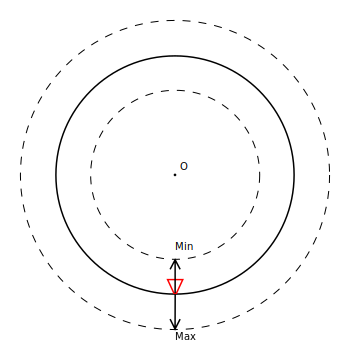
\includegraphics{distance_limits.png}
\end{figure}

\begin{DUlineblock}{0em}
\item[] 
\end{DUlineblock}

Default values: \emph{Min = 1, Max = 100}.

\begin{DUlineblock}{0em}
\item[] 
\end{DUlineblock}

\emph{Blend4Web \textgreater{} Use horizontal rotation clamping} -- available in the \code{Target} and \code{Eye} modes. Limits the camera's horizontal rotation relative to the pivot point (in the \code{Target} mode) or relative to its position (in the \code{Eye} mode).

The direction from \code{Left} to \code{Right} is considered positive and matches the counterclockwise direction for the \code{Target} mode, and the clockwise direction for the \code{Eye} mode:
\begin{figure}[htbp]
\centering

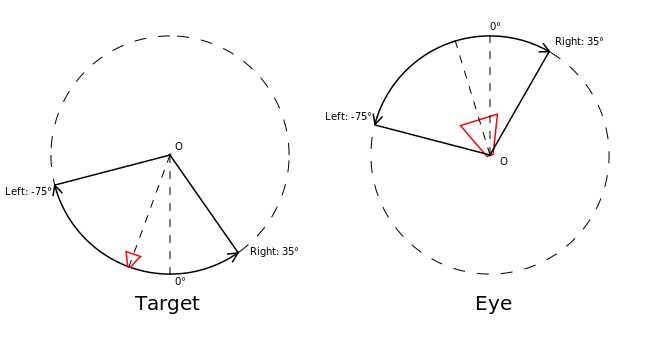
\includegraphics{horizontal_limits.png}
\end{figure}

Default values: \emph{Left = -180, Right = 180}.

\begin{DUlineblock}{0em}
\item[] 
\end{DUlineblock}

\emph{Blend4Web \textgreater{} Use vertical rotation clamping} -- available in the \code{Target} and \code{Eye} modes. Limits the camera's vertical rotation relative to the pivot point (in the \code{Target} mode) or relative to its position (in the \code{Eye} mode).

The direction from \code{Down} to \code{Up} is considered positive:
\begin{figure}[htbp]
\centering

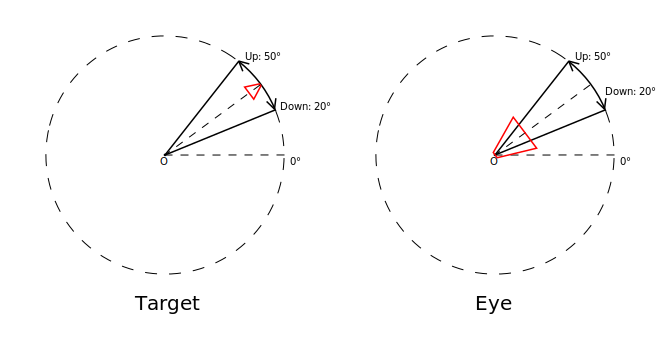
\includegraphics{vertical_limits.png}
\end{figure}

If the \emph{Use horizontal rotation clamping} checkbox is enabled, vertical rotation will be limited at least to the interval \emph{{[}-90, 90{]}}.

Default values: \emph{Down = -90, Up = 90}.

\begin{DUlineblock}{0em}
\item[] 
\end{DUlineblock}

\textbf{Possible rotation limits pitfalls}
\begin{itemize}
\item {} 
Swapping the \emph{Left/Right} or \emph{Down/Up} values swaps the rotations arcs.

\end{itemize}
\begin{figure}[htbp]
\centering


\includegraphics{limits_inversion.png}
\end{figure}
\begin{itemize}
\item {} 
\emph{Left = Right, Up = Down} - fixes the camera horizontally and vertically (respectively).

\end{itemize}

\begin{DUlineblock}{0em}
\item[] 
\end{DUlineblock}

\textbf{Rotation angles origin}

You can choose the space of coordinates for horizontal and vertical rotation limits:
\begin{itemize}
\item {} 
\code{Camera space} - all angles are measured relative to the initial camera position and orientation.

\item {} 
\code{World space} - horizontal angles are measured starting from the Y axis in the world space, while vertical angles - relative to the horizontal plane XOY in the world space.

\end{itemize}

For horizontal limits:
\begin{figure}[htbp]
\centering

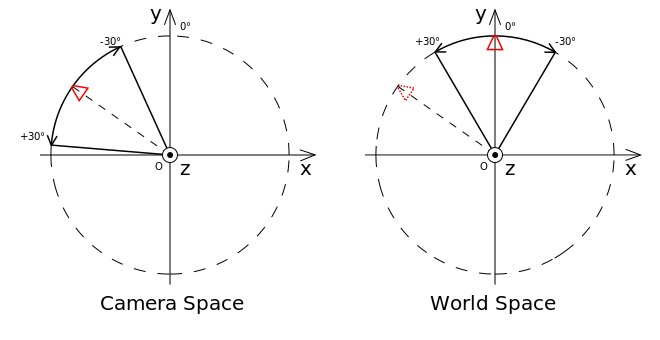
\includegraphics{camera_space_world_space_h.png}
\end{figure}

For vertical limits:
\begin{figure}[htbp]
\centering

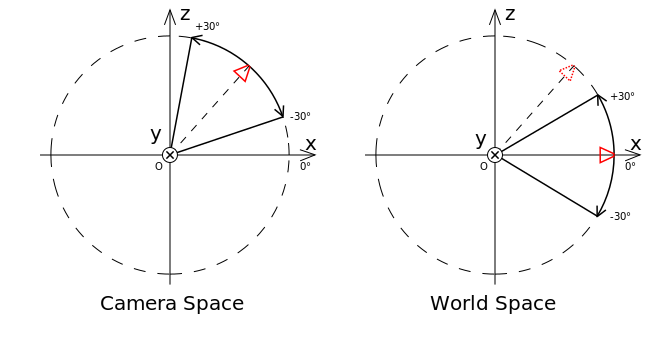
\includegraphics{camera_space_world_space_v.png}
\end{figure}

The coordinate axes labelled on the pictures match the Blender's world coordinate axes.

By default the \code{Camera space} option is selected.
\phantomsection\label{textures:textures}
\index{textures}

\chapter{Textures}
\label{textures:index-0}\label{textures::doc}\label{textures:id1}
\index{textures!types}

\section{Texture Types}
\label{textures:id2}\label{textures:index-1}
The \code{Type} drop-down menu (for selecting texture type) is located under the \code{Textures} tab. The engine supports the following texture types:
\begin{enumerate}
\item {} \begin{description}
\item[{\code{Image or Movie}}] \leavevmode\begin{itemize}
\item {} 
diffuse map

\item {} 
specular map, this can also be packed into the alpha channel of a diffuse texture

\item {} 
normal map

\item {} 
height map; this must be packed into the alpha channel of a normal map; it is used for relief surfaces visualization (parallax mapping).

\item {} 
transparency map (alpha map) - is used separately only for water rendering at low quality mode; in a generic material this is contained in the alpha channel of a diffuse texture

\item {} 
stencil map

\end{itemize}

\end{description}

\item {} \begin{description}
\item[{\code{Environment Map}}] \leavevmode\begin{itemize}
\item {} 
mirror map

\item {} 
{\hyperref[textures:skydome-texture]{\emph{skydome texture}}}

\end{itemize}

\end{description}

\item {} \begin{description}
\item[{\code{None}}] \leavevmode\begin{itemize}
\item {} 
applied to the Blender's default scene cube. A gray texture is generated in the engine. It is also used for {\hyperref[textures:render-to-texture]{\emph{rendering a scene to texture}}}.

\end{itemize}

\end{description}

\item {} \begin{description}
\item[{\code{Blend}, gradient}] \leavevmode\begin{itemize}
\item {} 
is used in {\hyperref[particles:particles-textures]{\emph{particle systems}}}

\end{itemize}

\end{description}

\item {} \begin{description}
\item[{\code{Voronoi} procedural texture type}] \leavevmode\begin{itemize}
\item {} 
is used for water rendering to setup the caustics effect

\end{itemize}

\end{description}

\end{enumerate}

\index{textures!settings}

\section{Generic Settings}
\label{textures:id3}\label{textures:index-2}\begin{description}
\item[{\emph{Dimensions}}] \leavevmode
Bitmap dimensions for image textures (image width and height in pixels) should be a 2$^{\text{N}}$ number, i.e. 4, 8, 16, 32, 64, 128, 256, 512, 1024, 2048, 4096 px. Using textures with other dimensions (so-called NPOT) is supported but is not recommended. Dimensions should be at least 4 pixels for the correct texture compression. Normally square images are used (e.g. 512 x 512 px), however rectangular ones can be used too (e.g. 4 x 128 px). Using images bigger than 2048 px is not recommended.

\item[{\emph{Image Mapping \textgreater{} Extension}}] \leavevmode
Texture coordinates interpretation mode (Wrap Mode in WebGL). This is available for \code{Image or Movie} texture type. In case of \code{Repeat} value the engine sets the \code{REPEAT} mode for the texture. In this case the integer part of the texture coordinates is ignored and the fractional part is used. In all other cases (for example \code{Extend}) the engine sets the \code{CLAMP\_TO\_EDGE} mode. In this case the texture coordinates are limited by the {[}0, 1{]} segment. The default value is \code{Repeat}.

\end{description}

\index{material capture}\index{matcap}\begin{description}
\item[{\emph{Mapping \textgreater{} Coordinates}}] \leavevmode
Texture coordinates type. Supported types are \code{UV} (use UV map), \code{Normal} (use direction at the camera; available only for diffuse maps; used for the creation of \textbf{material capture}, \textbf{matcap}). The default value is \code{Generated} (!).

\item[{\emph{Mapping \textgreater{} Offset}}] \leavevmode
Unsupported.

\item[{\emph{Mapping \textgreater{} Size}}] \leavevmode
Scaling the UV map along respective axes. The default values are 1.0.

\item[{\emph{Blend4Web \textgreater{} Do not export}}] \leavevmode
Do not export the texture. Disabled by default.

\item[{\emph{Blend4Web \textgreater{} Anisotropic Filtering}}] \leavevmode
Anisotropic filtering factor for the individual texture. It has priority over the similar parameter for the scene. The default value is \code{DEFAULT} (i.e. use the scene settings).

\item[{\emph{Blend4Web \textgreater{} UV translation velocity}}] \leavevmode
Animation speed of texture coordinates along respective axes. The default values are 0.0.

\item[{\emph{Blend4Web \textgreater{} Water Foam}}] \leavevmode
The foam texture. Used by the water rendering material.

\end{description}

\index{textures!diffuse}\index{diffuse map}

\section{Diffuse Map}
\label{textures:index-4}\label{textures:diffuse-map}
A diffuse map is used for specifying scattered light distribution (the Lambert model).


\subsection{Activation}
\label{textures:id4}
Enable the \code{Diffuse \textgreater{} Color} checkbox on the \code{Textures \textgreater{} Influence} panel.


\subsection{Additional settings}
\label{textures:id5}\begin{description}
\item[{\emph{Influence \textgreater{} Diffuse \textgreater{} Color}}] \leavevmode
Influence of the texture on the diffuse color. The default value is 1.0.

\item[{\emph{Influence \textgreater{} Blend}}] \leavevmode
The type of the interaction with the material color (\code{Material \textgreater{} Diffuse \textgreater{} Color}), or with the vertex color if the \code{Vertex Color Paint} checkbox is enabled. The following types are supported: \code{Mix} (mixes with the color), \code{Multiply} (multiplies by the color). The default value is \code{Mix}.

\end{description}

\index{textures!specular map}\index{specular map}

\section{Specular Map}
\label{textures:index-5}\label{textures:specular-map}
The specular map is used for specifying the reflected light color distribution (the Phong model).


\subsection{Activation}
\label{textures:id6}
Enable the \code{Specular \textgreater{} Color} checkbox on the \code{Textures \textgreater{} Influence} panel (the \code{Specular \textgreater{} Intensity} checkbox is not supported).


\subsection{Additional settings}
\label{textures:id7}\begin{description}
\item[{\emph{Influence \textgreater{} Specular \textgreater{} Color}}] \leavevmode
The influence of the texture on the reflected light color. The default value is 1.0.

\item[{\emph{Influence \textgreater{} Blend}}] \leavevmode
The type of interaction with the reflected light color of the material (\code{Material \textgreater{} Specular \textgreater{} Color}). \code{Mix} (mixes with the color) is the only supported type. The default value is \code{Mix}.

\end{description}

The specular map can be packed to the alpha channel of a diffuse texture for optimization purposes. In such case it is required for the texture to enable the \code{Diffuse \textgreater{} Color} and \code{Specular \textgreater{} Color} checkboxes simultaneously. The color range is limited by gray tints.

\index{textures!normal map}\index{normal map}

\section{Normal Map}
\label{textures:index-6}\label{textures:normal-map}
A normal map is used for specifying the distribution of surface normals (perpendiculars) with the purpose of the relief detalization. The information about the normals should be stored in the texture space of coordinates. Normal maps baked in the object space of coordinates are not supported.


\subsection{Activation}
\label{textures:id8}
Enable the \code{Geometry \textgreater{} Normal} checkbox on the \code{Textures \textgreater{} Influence} panel.


\subsection{Additional settings}
\label{textures:id9}\begin{description}
\item[{\emph{Influence \textgreater{} Geometry \textgreater{} Normal}}] \leavevmode
Normal map influence on the resulting normals calculation. The default value is 1.0.

\end{description}

\index{textures!height map}\index{height map}\index{parallax mapping}

\section{Height Map. Parallax Mapping}
\label{textures:index-7}\label{textures:height-map-parallax-mapping}
A height map contains information about the distribution of relative relief heights. The higher the surface level is, the brighter is its color. A height map combined with a normal map is required for the implementation of relief surface effect (parallax mapping). A height map should be present in the alpha channel of a normal map.


\subsection{Activation}
\label{textures:id10}
For the normal map enable the \code{Parallax} checkbox on the \code{Textures \textgreater{} Blend4Web} panel in addition to the \code{Geometry \textgreater{} Normal} checkbox on the \code{Textures \textgreater{} Influence} panel.


\subsection{Additional settings}
\label{textures:id11}\begin{description}
\item[{\emph{Blend4Web \textgreater{} Parallax Scale}}] \leavevmode
Influence factor for the relief surface effect. The default value is 0.03.

\item[{\emph{Blend4Web \textgreater{} Parallax Steps}}] \leavevmode
The number of iterations for the relief surface calculations. Bigger value leads to better quality but is more computationaly expensive.

\end{description}

{\hfill\includegraphics[width=1.000\linewidth]{parallax.jpg}\hfill}

\begin{DUlineblock}{0em}
\item[] 
\end{DUlineblock}

\index{textures!alpha map}\index{alpha map}

\section{Alpha Map}
\label{textures:alpha-map}\label{textures:texture-alpha-map}\label{textures:index-8}
The separate alpha map is used only for low quality water rendering. In a generic material it can be present in the alpha channel of a diffuse texture.


\subsection{Activation}
\label{textures:id12}
For the diffuse texture enable the \code{Diffuse \textgreater{} Alpha} checkbox on the \code{Textures \textgreater{} Influence} panel in addition to the \code{Diffuse \textgreater{} Color} checkbox. For the separate alpha map enable the \code{Diffuse \textgreater{} Alpha} checkbox.


\subsection{Additional settings}
\label{textures:id13}\begin{description}
\item[{\emph{Influence \textgreater{} Diffuse \textgreater{} Alpha}}] \leavevmode
Unsupported.

\item[{\emph{Influence \textgreater{} Blend}}] \leavevmode
Unsupported.

\end{description}

{\hfill\includegraphics[width=1.000\linewidth]{alpha_map_water.jpg}\hfill}

\begin{DUlineblock}{0em}
\item[] 
\end{DUlineblock}

\index{textures!stencil map}\index{stencil map}

\section{Stencil Map}
\label{textures:stencil-map}\label{textures:index-9}
The special purpose texture (colorful or grayscale) contains information about the distribution of other texture surfaces.


\subsection{Activation}
\label{textures:id14}\begin{enumerate}
\item {} 
In case of node materials a stencil map should be used in the corresponding node structure.

\item {} 
In case of generic materials a stencil map should be located in a texture slot between two mixed diffuse textures. A stencil map requires to set both the \code{RGB to Intensity} and the \code{Stencil} checkboxes on the \code{Textures \textgreater{} Influence} panel.

\end{enumerate}


\subsection{Additional settings}
\label{textures:id15}
In the case of generic materials one of the mixed diffuse textures can have the \code{Normal} (``matcap'') texture coordinates type.


\subsection{Limitations}
\label{textures:id16}
In case of generic materials the engine only interprets the red channel of a stencil map. Specular maps or normal maps (if any) are not being mixed. The \code{Mapping \textgreater{} Size} setting is extracted from the first texture and is applied to all remaining textures.


\subsection{Example}
\label{textures:id17}
The apple model material has the following textures: a normal map, a diffuse texture with a specular map in its alpha channel, a stencil map, a diffuse ``matcap'' map, an environment map.

{\hfill\includegraphics[width=1.000\linewidth]{stencil_apple.jpg}\hfill}

\begin{DUlineblock}{0em}
\item[] 
\end{DUlineblock}

{\hfill\includegraphics[width=1.000\linewidth]{stencil_apple_separate_textures.jpg}\hfill}

\begin{DUlineblock}{0em}
\item[] 
\end{DUlineblock}

\index{textures!environment map}\index{environment map}

\section{Environment Map}
\label{textures:environment-map}\label{textures:index-10}
An environment map is used as a mirror map and as a static sky texture (skydome).

The engine considers it as a cube texture. Environment map bitmaps should contain 6 projected environment images, packed in 2 rows 3 pieces in each (a Blender format). Bitmap dimensions for each image should follow the 2$^{\text{N}}$ rule (512, 1024 etc).

It is recommended to use the lossless format (PNG) in order to avoid seams.

{\hfill\includegraphics[width=1.000\linewidth]{environment_map.png}\hfill}


\subsection{Environment map creation}
\label{textures:id18}
Blender has an option for baking a scene into an environment map. To do this:
\begin{enumerate}
\item {} 
Create a scene for baking.

\item {} 
Add an empty object in the supposed point of view (\code{Add \textgreater{} Empty}).

\item {} 
Go to the \code{World} tab then to the \code{Textures} tab and create a new texture with the \code{Environment Map} type.

\item {} 
On the \code{Environment Map} panel select the \code{Static} source, then select the empty object in the \code{Viewport Object} field, then set the 2$^{\text{N}}$ dimension (512, 1024 etc).

\item {} 
Render the scene by pressing \code{F12} (a camera is required).

\item {} 
Save the environment map into a file.

\end{enumerate}

{\hfill\includegraphics[width=1.000\linewidth]{environment_map_baking_scene.jpg}\hfill}

\begin{DUlineblock}{0em}
\item[] 
\end{DUlineblock}

{\hfill\includegraphics[width=1.000\linewidth]{environment_map_baking_ui.jpg}\hfill}

\index{textures!mirror map}\index{mirror map}

\section{Mirror Map}
\label{textures:id19}\label{textures:mirror-map}\label{textures:index-11}
A mirror map is used to visualize the surface reflection. This is an environment map.


\subsection{Activation}
\label{textures:id20}
Select the \code{Environment Map} texture type (\code{Type}). Enable the \code{Shading \textgreater{} Mirror} checkbox on the \code{Textures \textgreater{} Influence} panel.


\subsection{Additional settings}
\label{textures:id21}\begin{description}
\item[{\emph{Influence \textgreater{} Shading \textgreater{} Mirror}}] \leavevmode
The degree to which the mirror map affects the reflection. The default value is 1.0.

\end{description}


\strong{See also:}


{\hyperref[materials:reflection-static]{\emph{Static reflection}}}.



\index{textures!sky}\index{skydome}

\section{Skydome}
\label{textures:skydome}\label{textures:skydome-texture}\label{textures:index-12}
A skydome is used to visualize the sky. This is an environment map.


\subsection{Activation}
\label{textures:id22}
Create a specially oriented plane model. Create a material and enable the \code{Blend4Web \textgreater{} Special: Skydome} checkbox. Create the \code{Environment Map} texture.


\subsection{Additional settings}
\label{textures:id23}
Enable the \code{Blend4Web \textgreater{} Disable frustum culling} checkbox for the plane object in order to avoid image disappearance upon camera rotation.

{\hfill\includegraphics[width=1.000\linewidth]{skydome.jpg}\hfill}

\begin{DUlineblock}{0em}
\item[] 
\end{DUlineblock}
\phantomsection\label{textures:render-to-texture}
\index{textures!render to}\index{render-to-texture}\index{RTT}

\section{Render-to-Texture, RTT}
\label{textures:render-to-texture-rtt}\label{textures:index-13}
A 3D scene's real-time rendered image can be used as a texture by an object from another scene (``main'' scene).


\subsection{Activation}
\label{textures:id24}\begin{enumerate}
\item {} 
Create an additional source scene, rename it for convenience, create a \code{World}, add the objects wanted, setup the camera view.

\item {} 
Set the \code{None} type for a texture of the target object on the main scene, and specify the source scene's name in the \code{Blend4Web \textgreater{} Source scene} field. Select the \code{UV} in the \code{Mapping \textgreater{} Coordinates} menu. Make sure that the target object mesh has a UV map.

\end{enumerate}

{\hfill\includegraphics[width=1.000\linewidth]{render_to_texture.jpg}\hfill}


\subsection{Limitations}
\label{textures:id25}
Note that there is a bug at the moment which requires both scenes to have at least one shared light source.
\phantomsection\label{materials:materials}
\index{materials}

\chapter{Materials}
\label{materials:index-0}\label{materials::doc}\label{materials:id1}
Materials describe the object surface's response to light and also contain information about its transparency, reflectivity, physical parameters and so on.

Meshes can have one or more materials. In case of multiple materials they can be assigned to different polygons in the \code{Edit Mode}. To do this select the needed polygons, select the needed material from the list and click the \code{Assign} button.

The following material types are supported: \code{Surface}, \code{Halo}.

\index{materials!shading parameters}

\section{Lighting Parameters}
\label{materials:id2}\label{materials:index-1}\label{materials:material-lighting-params}\begin{figure}[htbp]
\centering

\scalebox{0.500000}{\includegraphics{material_panel_shading.jpg}}
\end{figure}
\begin{description}
\item[{\emph{Diffuse \textgreater{} Color}}] \leavevmode
Diffuse light color. The default value is (0.8, 0.8, 0.8). It may interact with the diffuse map color.

\item[{\emph{Diffuse \textgreater{} Intensity}}] \leavevmode
Diffuse light intensity. The default value is 0.8.

\item[{\emph{Diffuse \textgreater{} Shader}}] \leavevmode
Diffuse shading algorithm. The engine supports the following algorithms: \code{Lambert}, \code{Oren-Nayar}, \code{Fresnel}. The default value is \code{Lambert}.

\item[{\emph{Specular \textgreater{} Color}}] \leavevmode
Specular light color. The default value is (1.0, 1.0, 1.0). It may interact with the specular map color.

\item[{\emph{Specular \textgreater{} Intensity}}] \leavevmode
Specular light intensity. The default value is 0.5.

\item[{\emph{Specular \textgreater{} Hardness}}] \leavevmode
Exponent in the specular shading calculation formula. The default value is 50. Note that the formula used in the engine differs slightly from the Blender's one.

\item[{\emph{Specular \textgreater{} Shader}}] \leavevmode
Specular shading algorithm. The engine supports the following algorithms: \code{CookTorr}, \code{Phong} - both are treated as the same, and \code{WardIso}. The default value is \code{CookTorr}.

\item[{\emph{Shading \textgreater{} Emit}}] \leavevmode
Emission intensity. The default value is 0.0.

\item[{\emph{Shading \textgreater{} Ambient}}] \leavevmode
Ambient influence factor on material. The default value is 1.0.

\item[{\emph{Shading \textgreater{} Shadeless}}] \leavevmode
When enabled, a material doesn't react to light. Disabled by default.

\item[{\emph{Game Settings \textgreater{} Backface Culling}}] \leavevmode
When enabled, poligons' back faces are not rendered by the engine. Enabled by default.

\item[{\emph{Options \textgreater{} Vertex Color Paint}}] \leavevmode
Mesh vertex color is used instead of the material diffuse color when the checkbox is enabled.

\end{description}

\index{materials!transparency}\index{transparency}

\section{Transparency}
\label{materials:id3}\label{materials:index-2}
\index{transparency!types}

\subsection{Types}
\label{materials:id4}\label{materials:index-3}
Transparency implementation type can be selected in the \code{Alpha Blend} menu on the \code{Materials \textgreater{} Game Settings} panel (in the \code{Blender Game} mode).

The engine supports the following transparency implementation types (sorted in the ascending order by performance):
\begin{description}
\item[{\emph{Alpha Sort}}] \leavevmode
Transparent with a gradient. The engine sorts the triangles by camera distance in order to render overlapping transparent surfaces correctly. This operation is computationally expensive. It is recommended to use this feature for closed transparent geometry (bottle, car glass etc).

\item[{\emph{Alpha Blend}}] \leavevmode
Transparent with a gradient. The sorting of triangles is not performed. It is recommended to use this feature for unclosed transparent geometry (water surface, decals).

\item[{\emph{Add}}] \leavevmode
Transparent with a gradient. The sorting of triangles is not performed. The engine disables writing to the depth buffer which causes transparent surfaces to be rendered in arbitrary order. It is recommended to use this feature for effects (particle systems, glowing beams).

\item[{\emph{Alpha Clip}}] \leavevmode
Transparent without a gradient. The engine discards pixels if their alpha is less than 0.5. The sorting of triangles is not performed. It is recommended to use this feature with a mask texture to visualize smaller details (tree leaves, grass).

\item[{\emph{Opaque}}] \leavevmode
Non-transparent. Alpha is ignored. This is the default value.

\end{description}

{\hfill\includegraphics[width=1.000\linewidth]{alpha_types.jpg}\hfill}

\index{transparency!setup}

\subsection{Additional settings}
\label{materials:index-4}\label{materials:id5}\begin{description}
\item[{\emph{Transparency}}] \leavevmode
Enabling the transparency checkbox is required for viewing transparent objects in Blender. The engine ignores this option - the \code{Alpha Blend} option is used instead.

\item[{\emph{Transparency \textgreater{} Alpha}}] \leavevmode
Material transparency level. The engine ignores this parameter (in contrast to Blender) if there is a diffuse texture - the alpha channel values of a texture are used instead.

\item[{\emph{Options \textgreater{} Z Offset}, depth offset}] \leavevmode
This option explicitly specifies relative positioning order of objects with \textbf{different} materials with the purpose of depth sorting. The option can take both negative and positive values. The more distant the object is the lesser parameter value should be to provide correct rendering. The default value is 0.0.

\item[{\emph{Transparency \textgreater{} Fresnel}}] \leavevmode
Fresnel power for transparency. It is exported but is not used at the moment.

\item[{\emph{Transparency \textgreater{} Blend}}] \leavevmode
Fresnel factor for transparency. It is exported but is not used at the moment.

\end{description}

\index{materials!reflection}\index{reflection}

\section{Reflection}
\label{materials:id6}\label{materials:index-5}\label{materials:material-mirror}
\index{reflection!static}

\subsection{Static reflection}
\label{materials:id7}\label{materials:index-6}\label{materials:reflection-static}
A surface reflects the same image no matter how the environment changes. For activation simply use the {\hyperref[textures:mirror-map]{\emph{mirror map}}}.


\strong{See also:}


{\hyperref[materials:fresnel]{\emph{Fresnel effect for reflection}}}



\index{reflection!dynamic}

\subsection{Dynamic reflection}
\label{materials:index-7}\label{materials:id8}
A surface reflects the selected objects in their current position. Only reflection from a plane is supported.


\subsubsection{Activation}
\label{materials:id9}\begin{enumerate}
\item {} 
Enable the \code{Render reflections} checkbox on the \code{Scene \textgreater{} Blend4Web} panel.

\item {} 
Add an empty object as a reflection plane by executing for example \code{Add \textgreater{} Empty \textgreater{} Single Arrow}. Rename it for convenience.

\item {} 
For \emph{reflective} objects enable the \code{Reflective} checkbox on the \code{Object \textgreater{} Blend4Web} panel and specify the empty object name in the \code{Reflection plane} field.

\item {} 
For the needed materials of the \emph{reflective} objects enable the \code{Mirror \textgreater{} Reflectivity} value.

\item {} 
For the \emph{reflexible} objects enable the checkbox \code{Reflexible} on the \code{Object \textgreater{} Blend4Web} panel.

\end{enumerate}

\begin{notice}{note}{Note:}
It is also recommended to enable the \code{World \textgreater{} Environment Lighting} checkbox.
\end{notice}


\subsubsection{Limitations}
\label{materials:id10}
Normal maps and shadows are ignored in the reflected image for optimization purposes.


\strong{See also:}


{\hyperref[materials:fresnel]{\emph{Fresnel effect for reflection}}}



\index{reflection!Fresnel effect}\index{Fresnel effect}

\subsection{Fresnel effect for reflection}
\label{materials:id11}\label{materials:fresnel}\label{materials:index-8}
The Fresnel effect manifests itself as the dependency of the intencity of passing and reflected light on the incidence angle. If the angle of incidence is close to zero (i.e. light falls almost at right angle to the surface) the passing light portion is large and the reflected light portion is small. On the contrary if the angle of incidence is close to 90 degrees (i.e. light falls almost parallel to the surface) almost all light is reflected.

The engine uses the approximate Schlick's formula:
\begin{quote}

R = R$_{\text{0}}$ + (1 − R$_{\text{0}}$)(1 - cos \(\theta\))$^{\text{N}}$, where

R - reflection coefficient,

R$_{\text{0}}$ - reflection coefficient in case of viewing at a right angle to the surface (i.e. when \(\theta\) = 0),

\(\theta\) - angle of incidence (which is equal to the angle of reflection under which light enters the camera), it is calculated by the engine in real-time,

N - exponent.
\end{quote}


\subsubsection{Settings}
\label{materials:id12}
Fresnel effect can be set up both for static and dynamic reflection.
\begin{description}
\item[{\emph{Mirror \textgreater{} Fresnel}}] \leavevmode
Fresnel power for reflection. This is the N exponent in the Schlick's formula. In Blender it is limited to values from 0 to 5. If this parameter is equal to zero the Fresnel effect is not observed and the \emph{full} reflection at all angles occurs. If this parameter is greater than zero, the material is less reflective when viewing surfaces at angles which are close to the right angle. The bigger this parameter is the bigger is the angle deviation from the right angle for which the Fresnel effect is observed.

\item[{\emph{Mirror \textgreater{} Blend}}] \leavevmode
Fresnel factor for reflection. It is reduced to R$_{\text{0}}$ in the Schlick's formula by the following expression: R$_{\text{0}}$ = 1 - \code{Blend} / 5. In Blender it is limited to values from 0 to 5. This parameter defines the Fresnel effect intensity: the bigger the \code{Blend} factor is, the more is the Fresnel effect influence. If it is equal to zero the Fresnel effect is not observed.

\end{description}

{\hfill\includegraphics[width=1.000\linewidth]{reflection_dynamic_and_fresnel.jpg}\hfill}

\begin{DUlineblock}{0em}
\item[] 
\end{DUlineblock}

\index{materials!special parameters}

\section{Parameters Specific to the Engine}
\label{materials:id13}\label{materials:index-9}
Located on the \code{Blend4Web} panel.
\begin{description}
\item[{\emph{Do not export}}] \leavevmode
Material is not to be exported.

\item[{\emph{Special: Water}}] \leavevmode
A special material for water rendering.

\item[{\emph{Special: Skydome}}] \leavevmode
A special material for sky rendering.


\strong{See also:}


{\hyperref[textures:skydome-texture]{\emph{Skydome}}}



\item[{\emph{Special: Collision}}] \leavevmode
A special material for collision geometry.


\strong{See also:}


{\hyperref[physics:physics]{\emph{Physics}}}



\item[{\emph{Double-sided Lighting}}] \leavevmode
Enables the double-sided lighting mode. This option is useful for non-transparent objects with a single-layered mesh.

\end{description}

\index{materials!halo}\index{halo}

\section{Halo Materials}
\label{materials:material-halo}\label{materials:index-10}\label{materials:halo}
Halo materials are used in particle systems and in static meshes. Using the halo in static meshes is described below.


\subsection{Activation}
\label{materials:id14}
Select the \code{Halo} type under the \code{Materials} tab. It's also recommended to select the transparency type with a gradient (\code{Add}, \code{Alpha Blend} or \code{Alpha Sort}).

{\hfill\includegraphics[width=1.000\linewidth]{halo.jpg}\hfill}


\subsection{Additional settings}
\label{materials:id15}\begin{description}
\item[{\emph{Halo \textgreater{} Alpha}}] \leavevmode
Material transparency factor. The default value is 1.0 (non-transparent).

\item[{\emph{Halo \textgreater{} Color}}] \leavevmode
Material color. The default value is (0.8, 0.8, 0.8) (almost white).

\item[{\emph{Halo \textgreater{} Seed}}] \leavevmode
Unused.

\item[{\emph{Halo \textgreater{} Size}}] \leavevmode
Particle size. The default value is 0.5.

\item[{\emph{Halo \textgreater{} Hardness}}] \leavevmode
Exponent for computing the gradient. Affects visible dimensions of particles. The default value is 50.

\item[{\emph{Halo \textgreater{} Add}}] \leavevmode
Unused.

\item[{\emph{Halo \textgreater{} Rings}}] \leavevmode
Use rings. Relative quantity and color can be set up.

\item[{\emph{Halo \textgreater{} Lines}}] \leavevmode
Use lines. Relative quantity and color can be set up.

\item[{\emph{Halo \textgreater{} Star Tips}}] \leavevmode
Use stars. The quantity of edges can be set up.

\item[{\emph{Blend4Web \textgreater{} Special: Stars}}] \leavevmode
Enables the starry sky rendering mode while the mesh is fixed relative to the camera. For the lamp it is also required to enable the \code{Blend4Web \textgreater{} Dynamic intensity} checkbox. Applications must set up the hours of darkness via API.

\item[{\emph{Blend4Web \textgreater{} Blending Height}}] \leavevmode
Height range for the fading of stars.

\item[{\emph{Blend4Web \textgreater{} Stars Minimum Height}}] \leavevmode
Minimum height in the object's local space at which stars are visible.

\end{description}
\phantomsection\label{node_materials:node-materials}
\index{node materials}

\chapter{Node Materials}
\label{node_materials:index-0}\label{node_materials::doc}\label{node_materials:id1}
Shader nodes extend significantly the potential of Blender's standard materials by means of presenting shading as a batch of basic transformations.

\index{materials!nodes}

\section{Standard Nodes}
\label{node_materials:id2}\label{node_materials:index-1}\label{node_materials:generic-node-materials}
\index{materials!nodes}
All Blender functions are supported except the following cases:
\begin{itemize}
\item {} 
\code{Geometry} - the \code{Local}, \code{Orco} and \code{Vertex Alpha} outputs are not supported.

\item {} 
\code{Material}, \code{Extended Material} - no more than one node per material is allowed; the \code{Refl}, \code{Ambient}, \code{SpecTra}, \code{Ray Mirror} inputs are not supported; the \code{AO} output is not supported.

\item {} 
\code{RGB Curves} is not supported.

\item {} 
\code{Vector Curves} is not supported.

\end{itemize}

In addition a poor performance of some nodes in real-time context should be taken into account. It is not recommended to use the following nodes:
\begin{itemize}
\item {} 
\code{Hue/Saturation}

\item {} 
\code{MixRGB} - the \code{Burn}, \code{Dodge}, \code{Value}, \code{Saturation}, \code{Hue}, \code{Color} types.

\end{itemize}

It is not recommended to create very complex materials especially if they use many \code{Geometry} or \code{Texture} nodes.


\section{Special Nodes}
\label{node_materials:custom-node-materials}\label{node_materials:id3}
\index{materials!nodes}
Special nodes extend the standard nodes' functionality in order to support the engine features. Special nodes are created as node groups (\code{Node groups} or \code{Node tree}) with specially determined names and input formats. All special nodes are gathered in the \code{special\_nodes.blend} file for convenience.


\subsection{LINEAR\_TO\_SRGB and SRGB\_TO\_LINEAR}
\label{node_materials:linear-to-srgb-srgb-to-linear}
Color correction from linear color space to sRGB space and back.


\strong{See also:}


{\hyperref[gamma_alpha:gamma-nodes]{\emph{Gamma Correction in Node Materials}}}




\subsection{REPLACE}
\label{node_materials:replace}
The node replaces the inputs depending on the working environment (i.e. Blender viewport or Blend4Web). When working in Blender the \code{Color1} input is connected to the \code{Color} output and the \code{Color2} input is ignored. On the contrary when working in the engine the inputs are interchanged (the \code{Color1} one is ignored and the \code{Color2} one is connected to the output). The node is intended to display one node structure in the viewport and another - in the engine.

As a rule it is used for normal mapping. Blender's node materials do not support a tangent space of coordinates. Therefore the only possible method to display normal maps in the viewport correctly is their usage inside the Material nodes.


\subsection{CLAMP}
\label{node_materials:clamp}
The node limits the output value. As a result all the output vector components take values from 0 to 1 inclusive.


\subsection{TIME}
\label{node_materials:time}
Provides the timeline counting from the engine start (in seconds). May be used for animating any parameters in the node materials.


\subsection{NORMAL\_VIEW}
\label{node_materials:normal-view}
The node transforms a normal into the camera's space of coordinates. Transformation is necessary because the engine defines all normals in the world space of coordinates. A normal should be used only for effects and not for connecting to the output of the \code{Material} or \code{Extended Material} nodes.


\subsection{PARALLAX}
\label{node_materials:parallax}
The node implements the texture coordinates offset using a height map.


\subsubsection{Input parameters}
\label{node_materials:id4}\begin{description}
\item[{\emph{UV}}] \leavevmode
Source texture coordinates

\item[{\emph{Height}}] \leavevmode
RGBA texture with a height map packed into the alpha channel.

\item[{\emph{Scale}}] \leavevmode
Texture coordinates offset factor

\item[{\emph{Steps}}] \leavevmode
The number of steps for iterative generation of texture coordinates offset. The bigger this value is the better is the final quality.

\end{description}


\subsubsection{Output parameters}
\label{node_materials:id5}\begin{description}
\item[{\emph{UV}}] \leavevmode
Resulting texture coordinates which are used as input for the texture nodes.

\end{description}


\subsection{TRANSLUCENCY}
\label{node_materials:translucency}
The node implements a translucency effect (with respect to light sources only) for thin objects such as cloth, leaves, paper etc. The effect consists of two parts: 1) brightening of the object side which is opposite to the light source and 2) appearance of a light spot right in the light source place.


\subsubsection{Input parameters}
\label{node_materials:id6}\begin{description}
\item[{\emph{Color}}] \leavevmode
One-channel texture which defines material heterogeneity - the white color denotes maximum translucency effect while the black color denotes its absence. White color is used by default.

\item[{\emph{Backside Factor}}] \leavevmode
Material color correction coefficient for the side which is opposite to the light source. It describes the color richness effect for the translucent areas.
\begin{itemize}
\item {} 
\emph{Backside Factor \textless{} 1} - brightening

\item {} 
\emph{Backside Factor = 1} - no correction

\item {} 
\emph{Backside Factor \textgreater{} 1} - darkening

\end{itemize}

The default value is 1.

\item[{\emph{Spot Hardness}}] \leavevmode
Light spot blurring factor. The bigger this value is the smaller is the spot and the sharper are the spot edges. The default value is 1000.

\item[{\emph{Spot Intensity}}] \leavevmode
Light spot intesity. The bigger this value is the brighter is the light spot. The default value is 1.

\item[{\emph{Spot Diffuse Factor}}] \leavevmode
Material diffuse color influence on the light spot color.
\begin{itemize}
\item {} 
\emph{Spot Diffuse Factor = 0} - the light spot has the diffuse color

\item {} 
\emph{Spot Diffuse Factor = 1} - the light spot color is white

\end{itemize}

The default value is 1.

\end{description}


\subsubsection{Output parameters}
\label{node_materials:id7}\begin{description}
\item[{\emph{Translucency}}] \leavevmode
The output should be connected to the \code{Translucency} input of the \code{Extended Material} node.

\end{description}
\phantomsection\label{lighting:lighting}
\index{lighting}

\chapter{Lighting and Shadows}
\label{lighting:index-0}\label{lighting::doc}\label{lighting:id1}
\index{light sources}

\section{Lighting with Light Sources}
\label{lighting:id2}\label{lighting:index-1}
A scene can have multiple (but not less than one) light sources of different types.


\subsection{Light source types}
\label{lighting:id3}
The following light source types are supported:
\begin{description}
\item[{\emph{Point}}] \leavevmode
Light propagates from one point uniformly to all directions with gradual attenuation.

\item[{\emph{Sun}}] \leavevmode
Light propagates from an infinite plane in one direction without attenuation.

\item[{\emph{Spot}}] \leavevmode
Light propagates from one point within the angular limit, with gradual attenuation.

\item[{\emph{Hemi}}] \leavevmode
Hemispherical. Light propagates from an infinite hemisphere without attenuation.

\end{description}


\subsection{Light source setup}
\label{lighting:id4}
Performed in the \code{Object Data} tab when a lamp object is selected.

{\hfill\includegraphics[width=1.000\linewidth]{lighting_setup.jpg}\hfill}

\begin{DUlineblock}{0em}
\item[] 
\end{DUlineblock}
\begin{description}
\item[{\emph{Color}}] \leavevmode
Light color. The default value is (1.0, 1.0, 1.0) (i.e. white).

\item[{\emph{Energy}}] \leavevmode
Radiation intensity. The default value is 1.0.

\item[{\emph{Falloff}}] \leavevmode
Attenuation type. The value is exported but the engine always uses \code{Inverse Square}. It is applicable to the \code{Point} and \code{Spot} light source types. The default value is \code{Inverse Square}.

\item[{\emph{Distance}}] \leavevmode
Attenuation parameter. It is applicable to the \code{Point} and \code{Spot} light source types. The default value is 25.0.

\item[{\emph{Spot Shape \textgreater{} Size}}] \leavevmode
Cone angle in degrees. It is applicable to the \code{Spot} light source type. The default value is 45º.

\item[{\emph{Spot Shape \textgreater{} Blend}}] \leavevmode
Parameter for blurring light spot edges. It is applicable to the \code{Spot} light source type. The default value is 0.15.

\item[{\emph{Blend4Web \textgreater{} Do not export}}] \leavevmode
Don't export the light source. Disabled by default.

\item[{\emph{Blend4Web \textgreater{} Generate shadows}}] \leavevmode
Use this light source for shadow calculation. Should be used when multiple light sources are present. Disabled by default.

\item[{\emph{Blend4Web \textgreater{} Dynamic intesity}}] \leavevmode
Use this light source for calculating the time of day. Applicable only to the \code{Sun} light source type. Disabled by default.

\end{description}


\section{Ambient Lighting}
\label{lighting:id5}
The engine uses a simple hemispherical lighting model in which horizon and zenith colors should be specified.


\subsection{Activation}
\label{lighting:id6}
Enable the \code{Environment Lighting} checkbox on the \code{World} tab.

{\hfill\includegraphics[width=1.000\linewidth]{lighting_environment.jpg}\hfill}


\subsection{Setup}
\label{lighting:id7}\begin{description}
\item[{\emph{Environment Lighting \textgreater{} Energy}}] \leavevmode
Ambient lighting intensity. The default value is 1.0.

\item[{\emph{Environment Lighting \textgreater{} Environment Color}}] \leavevmode
Ambient lighting source type - the supported types are \code{White} and \code{Sky Color}. If the \code{White} type is selected, both horizon and zenith colors are white. If the \code{Sky Color} type is selected, the horizon and zenith colors can be specified by means of the \code{World \textgreater{} Horizon Color} and \code{World \textgreater{} Zenith Color} color pickers. The default value is \code{White}.

\item[{\emph{World \textgreater{} Horizon Color} and \emph{World \textgreater{} Zenith Color}}] \leavevmode
Horizon and zenith colors. It is recommended to activate the \code{World \textgreater{} Blend Sky} option for better color selection.

\end{description}


\section{Shadows}
\label{lighting:id8}

\subsection{Activation}
\label{lighting:id9}\begin{enumerate}
\item {} 
Enable the \code{Blend4Web \textgreater{} Shadows Cast} checkbox under the \code{Object} tab for the objects which \textbf{cast} shadows.

\item {} 
Enable the \code{Blend4Web \textgreater{} Shadows Receive} checkbox under the \code{Object} tab for the objects which \textbf{receive} shadows.

\item {} 
Make sure that the \code{Blend4Web \textgreater{} Render shadows} checkbox is enabled in the \code{Scene} tab.

\end{enumerate}


\subsection{Setup}
\label{lighting:id10}\begin{description}
\item[{\emph{Direction}}] \leavevmode
If there are multiple light sources, it is recommended to specify the exact light source which is used for shadow calculations, by enabling the \code{Blend4Web \textgreater{} Generate shadows} checkbox under the \code{Object Data} tab for the selected lamp object.

\item[{\emph{Color}}] \leavevmode
The shadow color is determined by ambient lighting settings.

\end{description}

The following additional settings are on the \code{Blend4Web \textgreater{} Shadow Settings} panel of the \code{World} tab:


\subsubsection{Cascades}
\label{lighting:id11}
In order to provide acceptable shadow quality and to cover considerable space at the same time it is required to use multiple stages for shadow generation (cascades). Thus the best quality cascades are situated near the observer while the worst quality cascades are in the distance.

{\hfill\includegraphics[width=1.000\linewidth]{shadow_cascades.jpg}\hfill}

\begin{DUlineblock}{0em}
\item[] 
\end{DUlineblock}
\begin{description}
\item[{\emph{CSM number}}] \leavevmode
Number of shadow cascades. Supported from 1 to 4 cascades. The default value is 3.

\item[{\emph{CSM near}}] \leavevmode
The nearest boundary of shadow rendering. The default value is 0.1.

\item[{\emph{CSM far}}] \leavevmode
The furthest boundary of shadow rendering. The default value is 100.

\item[{\emph{CSM lambda}}] \leavevmode
The distribution factor of cascade boundaries. The values for the calculated cascade boundaries are displayed in the viewer under the \code{Shadows} tab. The default value is 0.875.

\end{description}


\subsubsection{Softened shadows}
\label{lighting:id12}\begin{description}
\item[{\emph{Visibility falloff}}] \leavevmode
Factor for the exponential decay of shadow visibility which depends on the distance between the casting and receiving points. It is used to reduce self-shadowing artefacts (i.e. when the castor and the receiver are the same object). The default value is 3500.0.

\item[{\emph{Blur depth size mult}}] \leavevmode
Blur kernel size. Affects the shadow softening ratio. The default value is 1.0.

\item[{\emph{Blur depth edge size}}] \leavevmode
Difference between samples (in texels) for the edge detection algorithm. Decreases haloing by excluding edges from blurring. The default value is 2.0.

\item[{\emph{Blur depth diff threshold}}] \leavevmode
Maximum of depth difference for the edge detection algorithm multiplied by 1000. Decreases haloing by excluding edges from blurring. The default value is 0.1.

\end{description}


\chapter{Postprocessing Effects}
\label{postprocessing_effects:postprocessing-effects}\label{postprocessing_effects::doc}\label{postprocessing_effects:id1}
\index{motion blur}\index{motion blur}

\section{Motion Blur}
\label{postprocessing_effects:id2}\label{postprocessing_effects:motion-blur}\label{postprocessing_effects:index-0}
The motion blur effect can be used to improve the realism of an interactive scene. It is displayed as picture blurring when the camera or objects move.


\subsection{Activation}
\label{postprocessing_effects:id3}
Enable the \code{Enable Motion Blur} checkbox on the \code{Scene \textgreater{} Blend4Web} panel.


\subsection{Additional settings}
\label{postprocessing_effects:id4}
On the \code{World \textgreater{} Blend4Web \textgreater{} Motion blur settings} panel:
\begin{description}
\item[{\emph{Motion blur factor}}] \leavevmode
Effect appearance ratio. The higher this value is the stronger is the motion blur.

\item[{\emph{Motion blur decay threshold}}] \leavevmode
Blur fade-out ratio. The higher this value is the more distinct is the effect. The default value is 0.01.

\end{description}

{\hfill\includegraphics[width=1.000\linewidth]{motion_blur.jpg}\hfill}

\begin{DUlineblock}{0em}
\item[] 
\end{DUlineblock}

\index{depth of field}\index{depth of field}\index{DOF}

\section{Depth of Field}
\label{postprocessing_effects:id5}\label{postprocessing_effects:dof}\label{postprocessing_effects:index-1}
The depth of field effect (DOF) can be used to accentuate a part of a scene. It is displayed as picture blurring nearer and further from the camera focus.


\subsection{Activation}
\label{postprocessing_effects:id6}\begin{enumerate}
\item {} 
Select an active camera and go to its settings panel (\code{Object Data}).

\item {} 
Then two options are available:
\begin{itemize}
\item {} 
Select an object to use as the camera's focus in the \code{Focus} menu of the \code{Depth of Field} panel. In this case moving away or approaching this object will cause a corresponding correction of the camera focus.

\item {} 
Set a non-zero value for the \code{Distance} on the \code{Depth of Field} panel (in Blender units = meters). In this case the camera focus will be located at this distance from the camera and will move together with it.

\end{itemize}

\end{enumerate}


\subsection{Additional settings}
\label{postprocessing_effects:id7}
On the \code{Object Data \textgreater{} Blend4Web} panel when the active camera is selected:
\begin{description}
\item[{\emph{DOF front distance}}] \leavevmode
The distance from the focus to the nearest plane (relative to the camera) behind which full blurring occurs (in meters). The default value is 1.0.

\item[{\emph{DOF rear distance}}] \leavevmode
The distance from the focus to the furthest plane (relative to the camera) behind which full blurring occurs (in meters). The default value is 1.0.

\item[{\emph{DOF power}}] \leavevmode
Blurring ratio. The default value is 3.0.

\end{description}

{\hfill\includegraphics[width=1.000\linewidth]{dof.jpg}\hfill}

\begin{DUlineblock}{0em}
\item[] 
\end{DUlineblock}

\index{screen-space ambient occlusion}\index{screen-space ambient occlusion}\index{SSAO}

\section{Screen-Space Ambient Occlusion}
\label{postprocessing_effects:index-2}\label{postprocessing_effects:ssao}\label{postprocessing_effects:id8}
The screen-space ambient occlusion (SSAO) effect can be used to fake complex light reflections from objects. The basis of this effect is that the space between close objects is less accessible for diffused light and hence is darker.


\subsection{Activation}
\label{postprocessing_effects:id9}
Enable the \code{Enable SSAO} checkbox on the \code{Scene \textgreater{} Blend4Web} panel.


\subsection{Additional settings}
\label{postprocessing_effects:id10}
On the \code{World \textgreater{} Blend4Web \textgreater{} SSAO Settings} panel:
\begin{description}
\item[{\emph{Radius Increase}}] \leavevmode
The spherical sampling radius multiply factor when transfering from the internal sampling ring to the external one. The default value is 1.7.

\item[{\emph{Dithering Amount}}] \leavevmode
Ratio for random noise mixing used for reducing strips. The default value is 0.1.

\item[{\emph{Gauss Center}}] \leavevmode
Mathematical expectation - Gauss distribution parameter for the depth difference between a pixel and a neighbouring sample. The default value is 0.2.

\item[{\emph{Gauss Width}}] \leavevmode
Standard deviation - Gauss distribution parameter for the depth difference between a pixel and a neighbouring sample. The default value is 2.0.

\item[{\emph{Gauss Width Left}}] \leavevmode
Standard deviation in case the depth difference is less than the mathematical expectation. The default value is 0.1.

\item[{\emph{Influence}}] \leavevmode
SSAO appearance factor. The default value is 0.7.

\item[{\emph{Distance Factor}}] \leavevmode
Factor of SSAO decay with distance. The default value is 0.0 (i.e. no decay).

\item[{\emph{Samples}}] \leavevmode
Number of samples (the more samples there are the better is the quality but the poorer is the performance). The default value is 16.

\end{description}

{\hfill\includegraphics[width=1.000\linewidth]{ssao.jpg}\hfill}

\begin{DUlineblock}{0em}
\item[] 
\end{DUlineblock}

\index{crepuscular rays}\index{crepuscular rays}\index{god rays}

\section{God Rays}
\label{postprocessing_effects:god-rays}\label{postprocessing_effects:id11}\label{postprocessing_effects:index-3}
The god rays effect (aka crepuscular rays) simulates well-known natural phenomenon - the shining of illuminated air parts.


\subsection{Activation}
\label{postprocessing_effects:id12}
Enable the \code{Enable God Rays} checkbox on the \code{Scene \textgreater{} Blend4Web} panel.


\subsection{Additional settings}
\label{postprocessing_effects:id13}
On the \code{World \textgreater{} Blend4Web \textgreater{} God Rays Settings} panel:
\begin{description}
\item[{\emph{God Rays Intensity}}] \leavevmode
The effect appearance factor. The default value is 0.7.

\item[{\emph{Maximum Ray Length}}] \leavevmode
Rays length factor. Defines the step between samples of radial blurring. The default value is 1.0.

\end{description}

{\hfill\includegraphics[width=1.000\linewidth]{god_rays.jpg}\hfill}

\begin{DUlineblock}{0em}
\item[] 
\end{DUlineblock}


\section{Bloom}
\label{postprocessing_effects:id14}
Bloom appears when a picture has elements with a very different brightness. A glowing halo is created around the bright details.


\subsection{Activation}
\label{postprocessing_effects:id15}
Enable the \code{Enable Bloom} checkbox on the \code{Scene \textgreater{} Blend4Web} panel.


\subsection{Additional settings}
\label{postprocessing_effects:id16}
On the \code{World \textgreater{} Blend4Web \textgreater{} Bloom Settings} panel:
\begin{description}
\item[{\emph{Key}}] \leavevmode
Bloom intensity.

\item[{\emph{Blur}}] \leavevmode
Bloom blurriness factor.

\item[{\emph{Edge Luminance}}] \leavevmode
The boundary value of an element's relative brightness above which the bloom effect appears.

\end{description}

{\hfill\includegraphics[width=1.000\linewidth]{bloom.jpg}\hfill}

\begin{DUlineblock}{0em}
\item[] 
\end{DUlineblock}

\index{glow}\index{glow}

\section{Glow}
\label{postprocessing_effects:index-4}\label{postprocessing_effects:id17}\label{postprocessing_effects:glow}
The glow effect consists of illuminating the outline of the certain objects with some color. As a result a glowing halo is created around the object.


\subsection{Activation}
\label{postprocessing_effects:id18}
The glow effect can be activated by an application via API. The different models can be applied such as constant glow, fading out glow, pulsatory glow and any other. In order to enable the glow effect on a certain object it's required to enable the \code{Selectable} checkbox on the \code{Object \textgreater{} Blend4Web} panel.


\subsection{Additional settings}
\label{postprocessing_effects:id19}
On the \code{Object \textgreater{} Blend4Web} panel:
\begin{description}
\item[{\emph{Glow duration}}] \leavevmode
Duration of the glow animation in seconds. The default value is 1.

\item[{\emph{Glow period}}] \leavevmode
Repeat period of the glow animation in seconds. The default value is 1.

\item[{\emph{Glow relapses}}] \leavevmode
The amount of the glow animation iterations. If the amount equals to 0 the animation is repeated forever. The default value is 0.

\end{description}

On the \code{World \textgreater{} Blend4Web} panel:
\begin{description}
\item[{\emph{Objects glow color}}] \leavevmode
Default effect color for all objects. The defaut value is (1,1,1).

\item[{\emph{Glow factor}}] \leavevmode
When this parameter decreases so does the thickness and the brightness of the halo around the object. The default value is 1.

\end{description}

These settings are taken as default when the glow effect is initiated via API.

{\hfill\includegraphics[width=1.000\linewidth]{glow.jpg}\hfill}

\index{anaglyph}\index{stereoscopic rendering}\index{anaglyph}

\section{Stereoscopic Rendering (Anaglyph)}
\label{postprocessing_effects:anaglyph}\label{postprocessing_effects:index-5}\label{postprocessing_effects:id20}

\subsection{Activation}
\label{postprocessing_effects:id21}
The stereoscopic rendering mode is intended for viewing the content using special glasses. It is activated by an application via API.


\subsection{Additional settings}
\label{postprocessing_effects:id22}
No.

{\hfill
\includegraphics[width=1.000\linewidth]{anaglyph.jpg}\hfill}

\begin{DUlineblock}{0em}
\item[] 
\end{DUlineblock}

\index{color correction}\index{color correction}

\section{Color Correction}
\label{postprocessing_effects:index-6}\label{postprocessing_effects:id23}\label{postprocessing_effects:color-correction}

\subsection{Activation}
\label{postprocessing_effects:id24}
Enable the \code{Enable Color Correction} checkbox on the \code{Scene \textgreater{} Blend4Web} panel.


\subsection{Additional settings}
\label{postprocessing_effects:id25}
On the \code{World \textgreater{} Blend4Web \textgreater{} Color Correction Settings} panel:
\begin{description}
\item[{\emph{Brightness}}] \leavevmode
The default value is 0.0.

\item[{\emph{Contrast}}] \leavevmode
The default value is 0.0.

\item[{\emph{Exposure}}] \leavevmode
The default value is 1.0.

\item[{\emph{Saturation}}] \leavevmode
The default value is 1.0.

\end{description}

{\hfill\includegraphics[width=1.000\linewidth]{color_correction.jpg}\hfill}

\begin{DUlineblock}{0em}
\item[] 
\end{DUlineblock}

\index{anti-aliasing}\index{anti-aliasing}

\section{Anti-Aliasing}
\label{postprocessing_effects:antialiasing}\label{postprocessing_effects:index-7}\label{postprocessing_effects:id26}
Anti-aliasing is used to reduce undesirable rendering artefacts (poor pixelization).


\subsection{Activation}
\label{postprocessing_effects:id27}
Enable the \code{Enable Antialiasing} on the \code{Scene \textgreater{} Blend4Web} panel.


\subsection{Additional settings}
\label{postprocessing_effects:id28}
The anti-aliasing method is assigned simultaneously with the selection of the engine performance profile.
\begin{itemize}
\item {} 
\emph{low quality} - anti-aliasing is disabled

\item {} 
\emph{high quality} - the anti-aliasing method is FXAA (Fast Approximate Anti-Aliasing) by Nvidia

\item {} 
\emph{maximum quality} - the anti-aliasing method is SMAA (Enhanced Subpixel Morphological Anti-Aliasing) by Crytek

\end{itemize}

{\hfill\includegraphics[width=1.000\linewidth]{antialiasing.jpg}\hfill}

\begin{DUlineblock}{0em}
\item[] 
\end{DUlineblock}
\phantomsection\label{particles:particles}
\index{particle system}

\chapter{Particle System}
\label{particles:index-0}\label{particles::doc}\label{particles:id1}
The particle system is intended to visualize phenomena which are caused by the movement of numerous small objects such as smoke, fire, water splashes and other.

{\hfill\includegraphics[width=1.000\linewidth]{particles_smoke.jpg}\hfill}

\begin{DUlineblock}{0em}
\item[] 
\end{DUlineblock}

A particle system requires an emitter - an object which defines the location and the direction of the outgoing particles flow.


\section{Use}
\label{particles:id2}

\subsection{Necessary steps}
\label{particles:id3}\begin{enumerate}
\item {} 
Add a mesh emitter to the scene.

\item {} 
Create a material for particles on the emitter, for example of the \code{Halo} type. The \code{Surface} material type with a mandatory diffuse texture is also supported.

\item {} 
Add a particle system on the emitter.

\item {} \begin{description}
\item[{Initiate the engine playback. Two options are available:}] \leavevmode\begin{itemize}
\item {} 
``cyclic emission'' - enable the \code{Blend4Web \textgreater{} Cyclic emission} checkbox for the particle system.

\item {} 
``non-cyclic animation'' - enable the \code{Blend4Web \textgreater{} Animation \textgreater{} Use default} checkbox for the emitter.

\end{itemize}

\end{description}

\end{enumerate}


\subsection{Recommended additional settings}
\label{particles:id4}\begin{enumerate}
\item {} 
Set the \code{Add} transparency type for the particles' material.

\item {} 
Disable emitter rendering if needed using the \code{Particles \textgreater{} Render \textgreater{} Emitter} checkbox.

\item {} 
If an emitter is required on a scene use additional materials for it. In this case select the particles' material in the \code{Particles \textgreater{} Render \textgreater{} Material} menu on the particles settings panel.

\item {} 
If the \code{Surface} material type is used it is required to add a diffuse texture (normally with the alpha channel) to this material. Select  \code{UV} in the \code{Mapping \textgreater{} Coordinates} menu.  Make sure that the emitter's mesh has a UV layer.

\end{enumerate}

{\hfill\includegraphics[width=1.000\linewidth]{particles_first_steps.jpg}\hfill}


\section{Setup}
\label{particles:id5}
The particle system parameters can be set up under the \code{Particles} tab. Multiple particle systems per emitter are supported.


\subsection{Basic settings}
\label{particles:id6}\begin{description}
\item[{\emph{Name}}] \leavevmode
Particle system name. The default name is ``ParticleSystem''.

\item[{\emph{Settings}}] \leavevmode
Reference to the settings datablock of the particle system. The datablock settings can be shared between different particle systems.

\item[{\emph{Type}}] \leavevmode
Particle system type: \code{Emitter} or \code{Hair}. \code{Hair} particle systems can be used to create numerous copies of an object (so called instancing). The default is \code{Emitter}.

\item[{\emph{Seed}}] \leavevmode
Index in the table of random numbers which are used for particle system generation. The default value is 0.

\end{description}


\subsection{Emission settings}
\label{particles:id7}\begin{description}
\item[{\emph{Emission \textgreater{} Number}}] \leavevmode
Number of particles. The default value is 1000.

\item[{\emph{Emission \textgreater{} Start}}] \leavevmode
The first frame after which the emission of particles starts. The default value is 1.0.

\item[{\emph{Emission \textgreater{} End}}] \leavevmode
The last frame after which the emission of particles ends. The default value is 200.0.

\item[{\emph{Emission \textgreater{} Lifetime}}] \leavevmode
The life time of particles measured in frames. The default value is 50.0.

\item[{\emph{Emission \textgreater{} Lifetime \textgreater{} Random}}] \leavevmode
The random factor for the life time. The default value is 0.0.

\item[{\emph{Emission \textgreater{} Emit From}}] \leavevmode
Emission source type. The following types are supported: \code{Verts} (emit from vertices), \code{Faces} (emit from polygons). The default is \code{Faces}.

\item[{\emph{Emission \textgreater{} Emit From \textgreater{} Distribution}}] \leavevmode
Emission distribution settings: \code{Jittered}, \code{Random}, \code{Grid}. Ignored by the engine. Internally the engine always uses \code{Random} distribution. The default is \code{Jittered}.

\end{description}

{\hfill\includegraphics[width=1.000\linewidth]{particles_settings.jpg}\hfill}


\subsection{Direction settings}
\label{particles:id8}
Only the following settings are supported:
\begin{description}
\item[{\emph{Velocity \textgreater{} Emitter Geometry \textgreater{} Normal}}] \leavevmode
Factor influencing the emission along the emitter's mesh normals. The default value is 1.0.

\item[{\emph{Velocity \textgreater{} Other \textgreater{} Random}}] \leavevmode
Factor of randomization for emission direction. The default value is 0.0.

\end{description}


\subsection{Rotation settings}
\label{particles:id9}
Only the following settings are supported:
\begin{description}
\item[{\emph{Rotation \textgreater{} Angular Velocity \textgreater{} Mode}}] \leavevmode
Mode for particle billboards self-rotating. The following modes are supported: \code{Velocity} (constant rotation speed), \code{Random} (random rotation), \code{None} (no rotation). The default is \code{Velocity}.

\item[{\emph{Rotation \textgreater{} Angular Velocity \textgreater{} Factor}}] \leavevmode
Factor of rotation velocity for particle billboards. The default value is 0.0.

\end{description}


\subsection{Physics settings}
\label{particles:id10}
Only the following settings are supported:
\begin{description}
\item[{\emph{Physics \textgreater{} Type}}] \leavevmode
Physics calculation type: \code{No}, \code{Newtonian}, \code{Keyed}, \code{Boids}, \code{Fluid}. Ignored by the engine. \code{Newtonian} physics is always used. The default is \code{Newtonian}.

\item[{\emph{Physics \textgreater{} Size}}] \leavevmode
Particle size. The default value is 0.05.

\item[{\emph{Physics \textgreater{} Mass}}] \leavevmode
Particle mass. Affects interaction with force fields (such as wind). The default value is 1.0.

\item[{\emph{Physics \textgreater{} Forces \textgreater{} Brownian}}] \leavevmode
Exported but not used by the engine.

\end{description}

{\hfill\includegraphics[width=1.000\linewidth]{particles_settings2.jpg}\hfill}


\subsection{Rendering settings}
\label{particles:id11}
Only the following settings are supported:
\begin{description}
\item[{\emph{Render \textgreater{} Material}}] \leavevmode
Menu for selecting the particle's material. Used for referencing to the particle' material in case multiple materials are used by the emitter. The default value is \code{Default Material}.

\item[{\emph{Render \textgreater{} Emitter}}] \leavevmode
Enables emitter rendering on the scene. Enabled by default.

\item[{\emph{Render \textgreater{} Type}}] \leavevmode
Particle rendering mode: \code{None}, \code{Halo}, \code{Line}, \code{Path}, \code{Object}, \code{Group}, \code{Billboard}. The engine supports the \code{Object} and the \code{Group} modes which are used for objects and groups instancing respectively. Other modes are ignored. It is recommended to use the \code{Billboard} mode for convenient display of billboards. The default is \code{Halo}.

\end{description}


\subsection{Supported settings for force fields influence}
\label{particles:id12}\label{particles:particles-force-fields}
Only the following settings are supported:
\begin{description}
\item[{\emph{Field Weights \textgreater{} Gravity}}] \leavevmode
Gravity influence factor (Earth's attraction). The default value is 1.0.

\item[{\emph{Field Weights \textgreater{} Wind}}] \leavevmode
Wind influence factor. A \code{Wind} force field source should be present (can be added using \code{Add \textgreater{} Force Field}). A particle system is also influenced by the wind direction and strength. The default value is 1.0.

\end{description}


\subsection{Engine specific settings}
\label{particles:id13}\begin{description}
\item[{\emph{Blend4Web \textgreater{} Do not export}}] \leavevmode
Unsupported.

\item[{\emph{Blend4Web \textgreater{} Cyclic emission}}] \leavevmode
The option enables the cyclic emission mode. It can be used for permanent effects (such as smoke, burning, water splashes). It is recommended to set the \code{Emission \textgreater{} Start} value to zero. Disabled by default.

\item[{\emph{Blend4Web \textgreater{} Random emission}}] \leavevmode
The option enables a random emission time for particles. Disabled by default.

\item[{\emph{Blend4Web \textgreater{} Billboard align}}] \leavevmode
The way billboards are oriented: \code{View} - follow the camera, \code{XY plane}, \code{YZ plane}, \code{ZX plane} - align to the corresponding plane (in the world coordinate system of Blender). The default is \code{View}.

\item[{\emph{Blend4Web \textgreater{} Dissolve intervals \textgreater{} Fade-in} and \emph{Fade-out}}] \leavevmode
Starting and ending intervals (measured in frames) for gradually increasing and decreasing the particles' transparency.

\end{description}


\section{Textures in Particle Systems}
\label{particles:id14}\label{particles:particles-textures}

\subsection{Textures of the particle's material}
\label{particles:id15}
For the \code{Surface} particle's materials it is \textbf{required} to have a diffuse texture (normally with an alpha-channel). In the \code{Mapping \textgreater{} Coordinates} menu choose the \code{UV} option.  Make sure that the emitter's mesh has a UV layer.

For the \code{Halo} particle's materials it is \textbf{possible} to use a \code{Blend} texture with a \code{Linear} gradient. In the \code{Mapping \textgreater{} Coordinates} menu choose the \code{Strand / Particle} option. It is required to enable \code{Ramp} on a texture. Up to 4 gradient control points are supported.

{\hfill\includegraphics[width=1.000\linewidth]{particles_settings_ramp_color.jpg}\hfill}


\subsection{Textures of particle systems}
\label{particles:id16}
Textures can also be used for setting up the behaviour of particle systems. Unlike textures for particle materials such textures belong to the particle system datablock, not to the material datablock. To create a texture for the particle system it is required to go \textbf{from} the \code{Particles} tab to the \code{Textures} tab and then to click the \code{New} button.

The only supported type of textures is \code{Blend} with a \code{Linear} gradient. \code{Ramp} should be enabled on the texture. Up to 4 gradient control points are supported.

On the \code{Influence} panel choose the parameter which is influenced by the texture. At the moment the only supported parameter is \code{Size}.

{\hfill\includegraphics[width=1.000\linewidth]{particles_settings_ramp_size.jpg}\hfill}

\begin{DUlineblock}{0em}
\item[] 
\end{DUlineblock}

The result of using gradient textures on the particle material and the particle system:

{\hfill\includegraphics[width=1.000\linewidth]{particles_gun.jpg}\hfill}

\href{http://www.blendswap.com/blends/view/13977}{The original model was taken from here}
\phantomsection\label{particles_instancing:particles-instancing}
\index{particle system}\index{instancing}\index{instancing}

\chapter{Particle System for Instancing Objects}
\label{particles_instancing:index-0}\label{particles_instancing::doc}\label{particles_instancing:id1}
A particle system can be used to create multiple object copies (so called instancing).

{\hfill\includegraphics[width=1.000\linewidth]{particles_instancing_example.jpg}\hfill}


\section{Particle System Setup}
\label{particles_instancing:id2}
\textbf{Activation}
\begin{enumerate}
\item {} 
Create a particle system of the \code{Hair} type on the emitter.

\item {} 
On the \code{Render} panel select the \code{Object} (or the \code{Group}) rendering type.

\item {} 
In the \code{Dupli Object} field (or in the \code{Dupli Group} field) select the object (or the object group) for instancing. Both local and linked objects (or groups) are supported.

\end{enumerate}

\textbf{Recommended additional settings}
\begin{enumerate}
\item {} 
For correct size displaying set the \code{Emission \textgreater{} Hair Length} and \code{Render \textgreater{} Size} parameters to 1.0.

\item {} 
For correct orientation temporarily enable the \code{Advanced} option, activate the \code{Rotation} panel and select \code{None} in the \code{Initial Orientation} menu. Disable the \code{Advanced} option. It is also recommended to enable the \code{Render \textgreater{} Rotation} option.

\end{enumerate}

{\hfill\includegraphics[width=1.000\linewidth]{particles_instancing_setup.jpg}\hfill}

\begin{DUlineblock}{0em}
\item[] 
\end{DUlineblock}

\textbf{Setup}
\begin{description}
\item[{\emph{Render \textgreater{} Use Count}}] \leavevmode
The option is available for groups of particle objects. When enabled the interface for setting the relative number of objects in a group is displayed. The engine doesn't reproduce the exact location of objects of set types.

\item[{\emph{Blend4Web \textgreater{} Random location and size}}] \leavevmode
The option enables randomization for the location and the size of the objects. If enabled the engine generates random coordinates and size (limited to the \(\pm\)25\% range) for the particle objects. If it is disabled then the current coordinates and sizes of the particle objects are exported and used. Enabled by default.

\item[{\emph{Blend4Web \textgreater{} Initial random rotation}}] \leavevmode
The option enables random rotation of the objects relative to the axis which is defined by the \code{Rotation type} parameter. If enabled the engine generates random rotation angles for the particle objects. If disabled the zero rotation angle is used. Enabled by default.

\item[{\emph{Blend4Web \textgreater{} Rotation type}}] \leavevmode\begin{description}
\item[{The axis for randomly turning the object (the option is available when the \code{Blend4Web \textgreater{} Initial random rotation} checkbox is set). 2 options are available:}] \leavevmode\begin{itemize}
\item {} 
\code{Z axis} - the objects are turned randomly around the vertical Z axis

\item {} 
\code{Random axis} - the objects are turned randomly around a random axis

\end{itemize}

\end{description}

The default is \code{Z axis}

\item[{\emph{Blend4Web \textgreater{} Rotation strength}}] \leavevmode\begin{description}
\item[{The coefficient defining the range of random rotation angles - counting from the direction towards the camera (the option is available when the \code{Blend4Web \textgreater{} Initial random rotation} checkbox is enabled). Examples:}] \leavevmode\begin{itemize}
\item {} 
\code{Rotation strength = 1} - the angles will lie within the \([-\pi, \pi]\) range

\item {} 
\code{Rotation strength = 0.5} - the angles will lie within the \([-0.5 \cdot \pi, 0.5 \cdot \pi]\) range

\item {} 
\code{Rotation strength = 0.1} - the angles will lie within the \([-0.1 \cdot \pi, 0.1 \cdot \pi]\) range

\end{itemize}

\end{description}

The default value is 1.

\item[{\emph{Blend4Web \textgreater{} Billboard}}] \leavevmode
Enables billboarding for particles. Disabled by default.

\item[{\emph{Blend4Web \textgreater{} Billboard type}}] \leavevmode\begin{description}
\item[{Billboarding type (the option is available when the \code{Blend4Web \textgreater{} Billboard} option is set). 3 types are available:}] \leavevmode\begin{itemize}
\item {} 
\code{Basic} - simple one-sided billboarding: particles will be turned with their front side to the observer

\item {} 
\code{Random} - random two-sided billboarding: particles will be more often turned with their front or rear side to the observer and less often with their side; also there will be a small random turn; this model was created specially for instancing grass

\item {} 
\code{Jittered} - one-sided billboarding with particles wavering along the plane which is turned to the observer; this model was created specially for instancing tree leaves

\end{itemize}

\end{description}

The default is \code{Basic}.

\item[{\emph{Blend4Web \textgreater{} Jitter amplitude}}] \leavevmode
The coefficient of the particle oscillation amplitude (the option is available when the \code{Jittered} type is selected from the \code{Blend4Web \textgreater{} Billboard type} menu). The bigger this parameter is the bigger is the oscillation amplitude. The default value is 0.

\item[{\emph{Blend4Web \textgreater{} Jitter frequency}}] \leavevmode
The particle oscillation frequency in hertz (the option is available when the \code{Jittered} type is selected from the \code{Blend4Web \textgreater{} Billboard type} menu). The default value is 0.

\item[{\emph{Blend4Web \textgreater{} Billboard geometry}}] \leavevmode\begin{description}
\item[{Billboard rotation type (the option is available when the \code{Blend4Web \textgreater{} Billboard} checkbox is set). 2 types are available:}] \leavevmode\begin{itemize}
\item {} 
\code{Spherical} - spherical billboarding i.e. particles are fully oriented to the observer and their rotation is unlimited

\item {} 
\code{Cylindrical} - cylindrical billboarding i.e. particles are rotating only around the vertical Z axis.

\end{itemize}

\end{description}

The default is \code{Spherical}.

\item[{\emph{Blend4Web \textgreater{} Dynamic Grass}}] \leavevmode
The option enables the dynamic grass rendering mode. Disabled by default.

\item[{\emph{Blend4Web \textgreater{} Wind bending}}] \leavevmode\begin{description}
\item[{Inheriting the wind bending settings by the particles:}] \leavevmode\begin{itemize}
\item {} 
\code{Parent} - inherited from the emitter

\item {} 
\code{Instance} - inherited from the particle object itself

\end{itemize}

\end{description}

The default is \code{Parent}.

\item[{\emph{Blend4Web \textgreater{} Shadows}}] \leavevmode\begin{description}
\item[{Inheriting the shadow settings by particles:}] \leavevmode\begin{itemize}
\item {} 
\code{Parent} - inherited from the emitter

\item {} 
\code{Instance} - inherited from the particle object itself

\end{itemize}

\end{description}

The default is \code{Parent}.

\item[{\emph{Blend4Web \textgreater{} Reflection}}] \leavevmode\begin{description}
\item[{Inheriting the reflection settings by particles:}] \leavevmode\begin{itemize}
\item {} 
\code{Parent} - inherited from the emitter

\item {} 
\code{Instance} - inherited from the particle object itself

\end{itemize}

\end{description}

The default is \code{Parent}.

\item[{\emph{Blend4Web \textgreater{} Vertex color}}] \leavevmode\begin{description}
\item[{Inheriting the vertex color from the emitter. Contains 2 fields:}] \leavevmode\begin{itemize}
\item {} 
\code{from} - the emitter's existing vertex color name

\item {} 
\code{to} - the particle's existing vertex color name

\end{itemize}

\end{description}

There is no inheritance by default.

\end{description}


\section{Grass}
\label{particles_instancing:id3}\label{particles_instancing:particles-grass}
Instancing of objects can be used for visualizing vast grass. In this case grass is rendered near the camera when it moves through the landscape.

{\hfill\includegraphics[width=1.000\linewidth]{dynamic_grass.jpg}\hfill}

\begin{DUlineblock}{0em}
\item[] 
\end{DUlineblock}

\textbf{Activation}
\begin{enumerate}
\item {} 
On a separate plane object create a particle system for object instancing. Enable the \code{Blend4Web \textgreater{} Dynamic Grass} option.

\item {} 
On the supposed landscape material enable the \code{Blend4Web \textgreater{} Terrain dynamic grass} option.

\end{enumerate}

\textbf{Setup}

It is recommended to create a few planes (for example 3) with sizes corresponding to the desired grass cascades (e.g. 100, 150 and 250 meters).

On the landscape \textbf{material} the following text fields get active when the \code{Blend4Web \textgreater{} Terrain dynamic grass} option is enabled:
\begin{description}
\item[{\emph{Dynamic grass size (R)}}] \leavevmode
Vertex color layer name of the landscape mesh which is intended for modifying the grass size. The size (i.e. height) of the grass is defined by gray tints - the brighter color the is the higher is the grass.

\item[{\emph{Dynamic grass color (RGB)}}] \leavevmode
Name of the landscape mesh's vertex color layer which is intended for grass tinting. The vertex color is multiplied by the grass material color. The \code{Influence \textgreater{} Blend} parameter for the grass material's diffuse texture should have the \code{Multiply} value.

\end{description}

Vertex color layers with such names should exist in the landscape mesh.

It is also recommended to disable rendering of the emitter (the \code{Render \textgreater{} Emitter} option).

{\hfill\includegraphics[width=1.000\linewidth]{dynamic_grass_setup.jpg}\hfill}


\section{Tree Leaves}
\label{particles_instancing:particles-leaves}\label{particles_instancing:id4}
Instancing suits the rendering of tree leaves well and allows to get a better level of detail.

{\hfill\includegraphics[width=1.000\linewidth]{tree_leaves.jpg}\hfill}

\begin{DUlineblock}{0em}
\item[] 
\end{DUlineblock}

\textbf{Activation}

Performed as described in the \code{Particle system setup -\textgreater{} Activation} section (see above). In this case the tree is the emitter and the leaves and the small branches are the particles.

Additionally the following operations should be performed for the emitter:
\begin{itemize}
\item {} 
create a vertex group which includes vertices on which the particles will be placed

\item {} 
create a vertex color layer for the wind bending parameters of the tree and the leaves

\item {} 
create a vertex color layer to be inherited by the particles (for example it can be used for tinting the particles)

\end{itemize}

\textbf{Setup}
\begin{enumerate}
\item {} 
\code{Random rotation settings}

\end{enumerate}

If the \code{Blend4Web \textgreater{} Initial random rotation} checkbox is enabled then it is recommended to select the vertical axis for random rotation - \code{Z axis} (the \code{Blend4Web \textgreater{} Rotation type} menu). The \code{Blend4Web \textgreater{} Rotation strength} value can be set too.
\begin{enumerate}
\setcounter{enumi}{1}
\item {} 
\code{Billboarding settings}

\end{enumerate}

It is recommended to enable billboarding, to set its type as \code{Jittered} (the \code{Blend4Web \textgreater{} Billboard type} menu) and to make it spherical - \code{Spherical} (the \code{Blend4Web \textgreater{} Billboard geometry} menu). The \code{Blend4Web \textgreater{} Jitter amplitude} and \code{Blend4Web \textgreater{} Jitter frequency} values can be set too.
\begin{enumerate}
\setcounter{enumi}{2}
\item {} 
\code{Particles location settings}

\end{enumerate}

It is recommended to select the \code{Verts} value from the \code{Emission \textgreater{} Emit From} menu, and to select in the \code{Vertex Group \textgreater{} Density} field the emitter's vertex group which defines the placing of particles. Also the \code{Blend4Web \textgreater{} Random location and size} checkbox shoud be disabled.
\begin{enumerate}
\setcounter{enumi}{3}
\item {} 
\code{Wind Bending settings}

\end{enumerate}

It is recommended to enable inheritance settings from the emitter - select the \code{Parent} in the \code{Blend4Web \textgreater{} Wind bending} menu. Then for the emitter on the \code{Object} panel enable the \code{Blend4Web \textgreater{} Wind bending} checkbox and setup the bending parameters. For a tree it is enough to specify the \code{Blend4Web \textgreater{} Main Bending \textgreater{} Angle} and \code{Blend4Web \textgreater{} Main Bending \textgreater{} Frequency} parameters and also a vertex color name for bending in the \code{Blend4Web \textgreater{} Main Bending \textgreater{} Main stiffness} field.
\begin{enumerate}
\setcounter{enumi}{4}
\item {} 
\code{Vertex color inheritance settings}

\end{enumerate}

For the emitter's vertex color to be inherited it is required to specify the emitter's vertex color name and the particle's vertex color name respectively in the \code{Blend4Web \textgreater{} Vertex Color \textgreater{} from} and \code{Blend4Web \textgreater{} Vertex Color \textgreater{} to} fields. The color of the emitter's vertex that is closest to the particle and specified in the \code{from} field will be copied and propagated into the \code{to} particle's vertex color layer, as a result.

The resulting vertex color layer with the \code{Blend4Web \textgreater{} Vertex Color \textgreater{} to} name may be used in the particle's node material for its tinting or other effects.

{\hfill\includegraphics[width=1.000\linewidth]{particle_settings.jpg}\hfill}
\phantomsection\label{animation:animation}
\index{animation}\index{animation}

\chapter{Animation}
\label{animation:index-0}\label{animation::doc}\label{animation:id1}
In general animation is changing the object's parameters in time. The engine supports the following types of animation:
\begin{itemize}
\item {} 
Object animation is the moving an object as a whole. The parameters that can be animated are the center coordinates (\code{Location}), the rotation's quaternion (\code{Rotation} in the \code{Quaternion(WXYZ)} mode) and scaling (\code{Scale}).

\item {} 
Skeletal animation, i.e. object deformation using bones. Animation of a standalone armature object is also supported (for parenting to bones).

\item {} 
Vertex animation. An object's deformations can be recorded as frames and then reproduced in the engine.

\item {} 
Audio sources parametrization. Speaker's \code{Volume} and \code{Pitch} can be animated.

\item {} 
Wind bending - a procedural animation. Described {\hyperref[outdoor_rendering:wind]{\emph{separately}}}.

\item {} 
Particle emission. Described in the {\hyperref[particles:particles]{\emph{corresponding section}}}.

\end{itemize}


\section{Animation Control}
\label{animation:id2}
There are two ways to control animation in the engine:
\begin{enumerate}
\item {} 
Automatically, using the \code{Animation: Use default} and \code{Animation: Cyclic} checkboxes in the object's properties. In this case an appropriate animation method will be chosen by the engine and the object's animation playback will start just after a scene is loaded. In case of skeletal animation the action which is assigned to the object in the \code{Action Editor} window is played by default.

\item {} 
In an application via API using the \code{animation} module methods.

\end{enumerate}

It's useful to use the \code{Animation} interface for tweaking animation. This is covered in the {\hyperref[viewer:viewer]{\emph{corresponding section}}}.


\section{Object Animation}
\label{animation:id3}
Animation keyframes can be added for an object motion in Blender and then reproduced in the engine.

The following keyframe types are supported:
\begin{itemize}
\item {} 
\emph{Location}

\item {} 
\emph{Rotation} -- the \code{Quaternion(WXYZ)} mode is required.

\item {} 
\emph{Scale} -- for correct results the scale factor should be the same along all 3 axes.

\item {} 
\emph{LocRot} -- a combination of \emph{Location} and \emph{Rotation}.

\item {} 
\emph{LocScale} -- a combination of \emph{Location} and \emph{Scale}.

\item {} 
\emph{LocRotScale} -- a combination of \emph{Location}, \emph{Rotation} and \emph{Scale}.

\item {} 
\emph{RotScale} -- a combination of \emph{Rotation} and \emph{Scale}.

\end{itemize}

If an object-mesh is animated it is required to enable the \code{Do not batch} checkbox under the object properties tab.


\section{Skinning and Skeletal Animation}
\label{animation:id4}
For skeletal animation both a mesh object and an armature object are needed. The four steps should be carried out:
\begin{enumerate}
\item {} 
Create the object's ``skeleton'' in the armature object.

\item {} 
Assign vertex groups in the mesh object and link them to the bones. This can be performed by weight painting for example.

\item {} 
Animate the bones in the pose mode of the armature object. The same keyframe types can be used as for the object animation.

\item {} 
When inverse kinematics (IK) or other nontrivial structures are used, an additional step is required to bake the animations (\code{Action} datablocks in Blender). Baking can be performed using the \code{B4W Animation Bake} interface located on the \code{Blend4Web} panel.

\end{enumerate}

{\hfill\includegraphics[width=1.000\linewidth]{baker.png}\hfill}

\begin{DUlineblock}{0em}
\item[] 
\end{DUlineblock}

Baking is performed with the armature object selected. Elements of the \code{B4W Animation Bake} interface:
\begin{itemize}
\item {} 
\emph{Clean keyframes} -- optimize the animation keyframes after baking. In case of incorrect results it's recommended to turn this option off.

\item {} 
window with the list of actions being baked -- bake only the actions which are listed, else - bake all the actions possible.

\item {} 
\emph{Name} -- the current action name from the list of actions being baked.

\item {} 
\emph{Bake} -- perform baking. If the process is completed successfully, actions with names of \emph{NAME\_B4W\_BAKED} type appear in the scene. These actions can be assigned to the armature object and played back in the engine. It's worth noting that appropriate functioning of such actions in Blender is not garanteed, although the \emph{Cons Mute}/\emph{Cons Unmute} interface can help in some cases.

\item {} 
\emph{Cons Mute}/\emph{Cons Unmute} -- switch bone constraints off/on. The tool can be used for testing the baked actions.

\end{itemize}


\section{Vertex Animation}
\label{animation:id5}
Allows to record any geometry changes of a mesh object. Note that every vertex animation frame counts as a mesh. It's not recommended to make a long animation for a high-poly mesh, as it can increase the size of the source and exported files significantly and can also slow down the work of the engine.

A special tool is used for baking vertex animation - \code{B4W Vertex Anim Baker} - located on the \code{Blend4Web} tools panel.

{\hfill\includegraphics[width=1.000\linewidth]{vertex_anim_baker.jpg}\hfill}


\section{Audio Source Parametrization}
\label{animation:id6}
In addition the following animation key types are supported for the speaker objects:
\begin{itemize}
\item {} 
\emph{Volume}

\item {} 
\emph{Pitch}

\end{itemize}

Audio sources parametering in essence follows object animation.


\chapter{Outdoor Rendering}
\label{outdoor_rendering:outdoor-rendering}\label{outdoor_rendering::doc}\label{outdoor_rendering:id1}

\section{Water}
\label{outdoor_rendering:id2}

\subsection{Activation}
\label{outdoor_rendering:id3}
For the supposed water material enable the \code{Blend4Web \textgreater{} Special: Water} option under the \code{Material} tab.

{\hfill\includegraphics[width=1.000\linewidth]{water_material_setup.jpg}\hfill}


\subsection{Basic settings}
\label{outdoor_rendering:id4}\begin{description}
\item[{\emph{Transparency}}] \leavevmode
It is recommended to enable the gradient transparency \code{Game Settings \textgreater{} Alpha Blend} and to tweak the \code{Transparency \textgreater{} Alpha} value.

\item[{\emph{Lighting parameters}}] \leavevmode
Lighting parameters for the water material can be set up as described in the {\hyperref[materials:material-lighting-params]{\emph{Lighting Parameters}}} section.

\end{description}


\subsection{Waves dynamics}
\label{outdoor_rendering:id5}
Waves simulation is carried out by normal maps with animated UVs (from 0 up to 4 pieces). For normal textures the only shared image is used - the textures differs only by the \code{Mapping \textgreater{} Size} and \code{Blend4Web \textgreater{} UV translation velocity} parameters. The water mesh should have a UV layer.
\begin{figure}[htbp]
\centering

\includegraphics[width=0.700\linewidth]{water_texture_setup_normal.jpg}
\end{figure}


\subsection{Surface wetting}
\label{outdoor_rendering:id6}
Is carried out automatically. To turn the effect on enable the \code{Wettable} checkbox on the needed materials.


\subsection{Reflection and Fresnel effect}
\label{outdoor_rendering:id7}
For the water material both static and dynamic reflection is supported as well as the Fresnel effect. See the {\hyperref[materials:material-mirror]{\emph{Reflection}}} section.

{\hfill\includegraphics[width=1.000\linewidth]{water_reflection_dynamic.jpg}\hfill}


\subsection{Shoreline smoothing}
\label{outdoor_rendering:id8}\begin{description}
\item[{\emph{Blend4Web \textgreater{} Water Settings \textgreater{} Shore smoothing}}] \leavevmode
Enable smoothing.

\item[{\emph{Blend4Web \textgreater{} Water Settings \textgreater{} Water absorb factor}}] \leavevmode
Light absorption coefficient for the water. The higher it is the more transparent isthe water.

\end{description}

In the low quality mode an {\hyperref[textures:texture-alpha-map]{\emph{alpha map}}} can be used instead of this option.


\subsection{Color gradient}
\label{outdoor_rendering:id9}
For color gradient the water material should have a texture with the \code{Blend4Web \textgreater{} Shore distance map} option enabled which can be generated using the script for {\hyperref[outdoor_rendering:shore-distance-bake]{\emph{baking shoreline parameters}}}.
\begin{description}
\item[{\emph{Blend4Web \textgreater{} Water Settings \textgreater{} Shallow water color}}] \leavevmode
Shallow water color.

\item[{\emph{Blend4Web \textgreater{} Water Settings \textgreater{} Shallow water color factor}}] \leavevmode
Shallow water color mixing factor.

\item[{\emph{Blend4Web \textgreater{} Water Settings \textgreater{} Shore water color}}] \leavevmode
Water color just at the shore line.

\item[{\emph{Blend4Web \textgreater{} Water Settings \textgreater{} Shore water color factor}}] \leavevmode
Factor for mixing water color just near the shoreline.

\end{description}


\subsection{Refraction}
\label{outdoor_rendering:id10}
Under the \code{Scene} tab enable the \code{Blend4Web \textgreater{} Render refractions} checkbox.

{\hfill\includegraphics[width=1.000\linewidth]{water_refraction.jpg}\hfill}


\subsection{Foam}
\label{outdoor_rendering:id11}

\subsubsection{Activation}
\label{outdoor_rendering:id12}
For creating foam add two diffuse textures into the water material slots. For these textures enable the \code{Blend4Web \textgreater{} Water Foam} option.
\begin{figure}[htbp]
\centering

\scalebox{0.700000}{\includegraphics{water_texture_setup_foam.jpg}}
\end{figure}


\subsubsection{Setting up the textures}
\label{outdoor_rendering:id13}\begin{description}
\item[{\emph{Influence \textgreater{} Color}}] \leavevmode
Texture color influence factor. The default value is 1.0.

\item[{\emph{Blend4Web \textgreater{} UV Frequency}}] \leavevmode
Oscillation frequency of the animated UV coordinates. The default value is (1.0, 1.0).

\item[{\emph{Blend4Web \textgreater{} UV Magnitude}}] \leavevmode
Oscillation amplitude of the animated UV coordinates. The default value is (1.0, 1.0).

\end{description}


\subsubsection{Setting up the material}
\label{outdoor_rendering:id14}\begin{description}
\item[{\emph{Blend4Web \textgreater{} Water Settings \textgreater{} Water foam factor}}] \leavevmode
General influence factor for the foam. The default value is 0.5.

\end{description}


\subsection{Caustics and chromatic aberration}
\label{outdoor_rendering:id15}
To create the caustics effect add one \code{Voronoi} type texture to the water material slot.

{\hfill\includegraphics[width=1.000\linewidth]{water_caustics.jpg}\hfill}


\subsubsection{Setting up}
\label{outdoor_rendering:id16}\begin{figure}[htbp]
\centering

\scalebox{0.800000}{\includegraphics{water_texture_setup_caustics.jpg}}
\end{figure}
\begin{description}
\item[{\emph{Voronoi \textgreater{} Coloring: Intensity}}] \leavevmode
Caustics influence factor. The default value is 1.0.

\item[{\emph{Voronoi \textgreater{} Noise: Size}}] \leavevmode
Cell size for the procedural texture. The default value is 0.25.

\item[{\emph{Blend4Web \textgreater{} UV translation velocity}}] \leavevmode
Texture coordinates animation speed. The default value is (0.0, 0.0).

\end{description}


\subsection{Underwater environment}
\label{outdoor_rendering:id17}
{\hfill\includegraphics[width=1.000\linewidth]{underwater.jpg}\hfill}


\subsubsection{Visibility settings (``fog'')}
\label{outdoor_rendering:id18}\begin{description}
\item[{\emph{Blend4Web \textgreater{} Water Settings \textgreater{} Underwater fog density}}] \leavevmode
Exponential factor which affects the density and visibility distance. The default value is 0.06.

\item[{\emph{Blend4Web \textgreater{} Water Settings \textgreater{} Underwater fog color}}] \leavevmode
Fog color. The default value is (0.5, 0.5, 0.5) (gray).

\end{description}

The {\hyperref[postprocessing_effects:god-rays]{\emph{god rays effect}}} settings are also applied.


\subsection{Boundary between environments}
\label{outdoor_rendering:id19}
Disable the \code{Game Settings \textgreater{} Backface Culling} option.

{\hfill\includegraphics[width=1.000\linewidth]{water_border.jpg}\hfill}


\subsection{Volumetric waves}
\label{outdoor_rendering:id20}\label{outdoor_rendering:water-volumetric-waves}

\subsubsection{Activation}
\label{outdoor_rendering:id21}
\emph{Blend4Web \textgreater{} Water Settings \textgreater{} Water Dynamic}

Enable volumetric waves.

{\hfill\includegraphics[width=1.000\linewidth]{water_waves.jpg}\hfill}


\subsubsection{Setting up}
\label{outdoor_rendering:id22}\begin{description}
\item[{\emph{Blend4Web \textgreater{} Water Settings \textgreater{} Wave height}}] \leavevmode
Wave height. The default value is 0.0.

\item[{\emph{Blend4Web \textgreater{} Water Settings \textgreater{} Wave length}}] \leavevmode
Wave length. The default value is 10.0.

\item[{\emph{Blend4Web \textgreater{} Water Settings \textgreater{} Dist noise scale 0}}] \leavevmode
Size of the first component of the open water waves.

\item[{\emph{Blend4Web \textgreater{} Water Settings \textgreater{} Dist noise scale 1}}] \leavevmode
Size of the second component of the open water waves.

\item[{\emph{Blend4Web \textgreater{} Water Settings \textgreater{} Dist noise freq 0}}] \leavevmode
Frequency of the first component of the open water waves.

\item[{\emph{Blend4Web \textgreater{} Water Settings \textgreater{} Dist noise freq 1}}] \leavevmode
Frequency of the second component of the open water waves.

\item[{\emph{Blend4Web \textgreater{} Water Settings \textgreater{} Dir min shore fac}}] \leavevmode
Minimum height decrease coefficient of the shore waves.

\item[{\emph{Blend4Web \textgreater{} Water Settings \textgreater{} Dir frequency}}] \leavevmode
Frequency of the rolling of the shore waves.

\item[{\emph{Blend4Web \textgreater{} Water Settings \textgreater{} Dir noise scale}}] \leavevmode
Noise size for the shore waves.

\item[{\emph{Blend4Web \textgreater{} Water Settings \textgreater{} Dir noise freq}}] \leavevmode
Noise frequency for the shore waves.

\item[{\emph{Blend4Web \textgreater{} Water Settings \textgreater{} Dir min noise fac}}] \leavevmode
Noise minimum for the shore waves.

\item[{\emph{Blend4Web \textgreater{} Water Settings \textgreater{} Dist min fac}}] \leavevmode
Minimum coefficient of mixing for open water waves.

\item[{\emph{Blend4Web \textgreater{} Water Settings \textgreater{} Waves horizontal factor}}] \leavevmode
Coefficient that shows how much the shore waves are shifted in the shoreline direction.

\end{description}


\subsection{Generated surface settings}
\label{outdoor_rendering:id23}\begin{description}
\item[{\emph{Blend4Web \textgreater{} Water Settings \textgreater{} Generate mesh}}] \leavevmode
Enable generated surface.

\item[{\emph{Blend4Web \textgreater{} Water Settings \textgreater{} Number of cascades}}] \leavevmode
Number of cascades in the generated surface.

\item[{\emph{Blend4Web \textgreater{} Water Settings \textgreater{} Detailed distance}}] \leavevmode
Maximum distance from camera to the last cascades edge.

\end{description}

\index{shore line parameters}\index{shore line}

\subsubsection{Creating a texture with shoreline parameters.}
\label{outdoor_rendering:index-0}\label{outdoor_rendering:id24}\label{outdoor_rendering:shore-distance-bake}
On the tools panel (hotkey ``T'') under the \code{Blend4Web} tab open the \code{B4W Shore Distance Baker} panel. Set the parameters: maximum distance to shore (\code{Maximum Distance}) and the resulting texture size (\code{Texture Size}). Select a landscape object (or multiple objects) first, and then - a water object. Click the \code{Bake Shore Distance} button.

Depending on the texture size and the number of vertices in the processed meshes the execution time of the script may vary from a fraction of a second up to several minutes. Make sure that the texture named \code{ShoreDistance} is created for the water mesh.

Upon script execution some system properties are saved in the water material. Therefore the scene must be saved after the script has finished working.


\section{Atmosphere}
\label{outdoor_rendering:id25}

\subsection{Scattering}
\label{outdoor_rendering:id26}
Create a plane object for the skydome as specified in the {\hyperref[textures:skydome-texture]{\emph{Skydome}}} section. An environment map is not needed. Enable the \code{Special: Skydome} and \code{Procedural skydome} checkboxes on the material.

{\hfill\includegraphics[width=1.000\linewidth]{skydome_procedural.jpg}\hfill}

\begin{DUlineblock}{0em}
\item[] 
\end{DUlineblock}

The settings are located under the \code{World} tab.
\begin{description}
\item[{\emph{Sky Settings \textgreater{} Sky color}}] \leavevmode
Base sky color. The default value is (0.087, 0.255, 0.6) (blue).

\item[{\emph{Sky Settings \textgreater{} Rayleigh brightness}}] \leavevmode
Rayleigh scattering brightness (i.e. scattering on small particles). The default value is 3.3.

\item[{\emph{Sky Settings \textgreater{} Mie brightness}}] \leavevmode
Mie scattering brightness (i.e. scattering on large particles). The default value is 0.1.

\item[{\emph{Sky Settings \textgreater{} Spot brightness}}] \leavevmode
Sun spot brightness. The default value is 20.0.

\item[{\emph{Sky Settings \textgreater{} Scatter strength}}] \leavevmode
Light scattering factor. The default value is 0.2.

\item[{\emph{Sky Settings \textgreater{} Rayleigh strength}}] \leavevmode
Rayleigh scattering factor. The default value is 0.2.

\item[{\emph{Sky Settings \textgreater{} Mie strength}}] \leavevmode
Mie scattering factor. The default value is 0.006.

\item[{\emph{Sky Settings \textgreater{} Rayleigh collection power}}] \leavevmode
Rayleigh scattering exponent. The default value is 0.35.

\item[{\emph{Sky Settings \textgreater{} Mie collection power}}] \leavevmode
Mie scattering exponent. The default value is 0.5.

\item[{\emph{Sky Settings \textgreater{} Mie distribution}}] \leavevmode
Mie scattering distribution. The default value is 0.4.

\end{description}


\subsection{Fog}
\label{outdoor_rendering:id27}
Can be set up under the \code{World} tab.
\begin{description}
\item[{\emph{Blend4Web \textgreater{} Fog Settings \textgreater{} Fog density}}] \leavevmode
Exponential factor which affects density and the visibility distance. The default value is 0.0.

\item[{\emph{Blend4Web \textgreater{} Fog Settings \textgreater{} Fog color}}] \leavevmode
Fog color. The default value is (0.5, 0.5, 0.5) (gray).

\end{description}

When a dynamic skydome is used the fog color is defined by the sky color.


\subsection{Time of day}
\label{outdoor_rendering:id28}
Enable the \code{Blend4Web \textgreater{} Dynamic intensity} checkbox for the lamp.

Time of day can be set by applications via API. Particularly time of day can be set using the \code{Lighting} interface of the {\hyperref[viewer:viewer]{\emph{Scene viewer}}}.

{\hfill\includegraphics[width=1.000\linewidth]{sunset.jpg}\hfill}


\subsection{Stars}
\label{outdoor_rendering:id29}
Stars setup is described in the {\hyperref[materials:material-halo]{\emph{Halo Materials}}} section.

{\hfill\includegraphics[width=1.000\linewidth]{stars.jpg}\hfill}


\section{Wind}
\label{outdoor_rendering:id30}\label{outdoor_rendering:wind}\begin{description}
\item[{Wind strength and direction affect}] \leavevmode\begin{itemize}
\item {} 
{\hyperref[outdoor_rendering:wind-bending]{\emph{grass and tree leaves animation}}}

\item {} 
{\hyperref[particles:particles-force-fields]{\emph{particle system dynamics}}}

\item {} 
{\hyperref[outdoor_rendering:water-volumetric-waves]{\emph{water waves rolling frequency}}} (at the moment only strength is taken into account)

\end{itemize}

\end{description}


\subsection{Activation}
\label{outdoor_rendering:id31}
Add a force field object of the \code{Wind} type.


\subsection{Setting up}
\label{outdoor_rendering:id32}\begin{description}
\item[{\emph{Direction}}] \leavevmode
Direction can be set by rotating the force field object.

\item[{\emph{Force Fields \textgreater{} Strength}}] \leavevmode
Wind strength. Located under the \code{Physics} tab. The default value is 1.0.

\end{description}


\subsection{Grass and tree leaves animation}
\label{outdoor_rendering:wind-bending}\label{outdoor_rendering:id33}
Authoring resources for grass rendering is described in the {\hyperref[particles_instancing:particles-grass]{\emph{Grass}}} section.


\subsubsection{Activation}
\label{outdoor_rendering:id34}
Enable the \code{Blend4Web \textgreater{} Wind bending} checkbox for the grass or tree object.


\subsubsection{Setting up}
\label{outdoor_rendering:id35}
The interface panel becomes visible after the activation of the \code{Blend4Web \textgreater{} Wind bending} checkbox.

{\hfill\includegraphics[width=1.000\linewidth]{wind_bending_setup.jpg}\hfill}

\begin{DUlineblock}{0em}
\item[] 
\end{DUlineblock}
\begin{description}
\item[{\emph{Main bending \textgreater{} Angle}}] \leavevmode
Angle amplitude of the ``main'' deviation under the influence of wind (in degrees). The default value is 10.0.

\item[{\emph{Main bending \textgreater{} Frequency}}] \leavevmode
Frequency of the ``main'' deviation under the influence of wind. The default value is 0.25.

\item[{\emph{Main bending \textgreater{} Main stiffness (A)}}] \leavevmode
Text field for specifying the name of the vertex color layer which contains the information about the stiffness of the ``main'' deviation. Can be left empty.

\item[{\emph{Detail bending \textgreater{} Detail amplitude}}] \leavevmode
Angle amplitude of the ``detail'' deviation caused by the influence of wind (in degrees). The default value is 0.1.

\item[{\emph{Detail bending \textgreater{} Branch amplitude}}] \leavevmode
Angle amplitude of the branch deviation caused by the influence of wind (in degrees). The default value is 0.3.

\item[{\emph{Detail bending \textgreater{} Leaves stiffness (R)}}] \leavevmode
Text field for specifying the name of the vertex color layer which contains the information about the stiffness of leaves. Can be left empty.

\item[{\emph{Detail bending \textgreater{} Leaves phase (G)}}] \leavevmode
Text field for specifying the name of the vertex color layer which contains the information about the phase of leaves deviation. Can be left empty.

\item[{\emph{Detail bending \textgreater{} Overall stiffness (B)}}] \leavevmode
Text field for specifying the name of the vertex color layer which contains the information about the overall stiffness of leaves. Can be left empty.

\end{description}

Vertex color layers should be present in the mesh if their names are specified.

{\hfill\includegraphics[width=1.000\linewidth]{wind_bending_vcolors.jpg}\hfill}


\chapter{Gamma Correction and Alpha Compositing}
\label{gamma_alpha::doc}\label{gamma_alpha:gamma}\label{gamma_alpha:id1}

\section{Overview}
\label{gamma_alpha:id2}
The essence of gamma correction is packing the image brightness channel into 8 bits of information.

Graphics editors normally work in a non-linear color space where the darker components are encoded using more bits than the brighter ones. That means that a bigger RGB value corresponds to 0.5 of the real light intensity (a physical quantity called illuminance) - in a simplest case this value equals to 0.5 \textasciicircum{} (1/2.2) = 0.73.

{\hfill\includegraphics[width=1.000\linewidth]{gamma.jpg}\hfill}

\begin{DUlineblock}{0em}
\item[] 
\end{DUlineblock}

Images are always stored in a non-linear space because if they were not, 8 bits of information would not be enough to encode the light intensity and it would result in a wrong rendering of the darker tints.

Web browsers work in a non-linear space.

When the \code{Color Management \textgreater{} Display Device \textgreater{} sRGB} option is enabled for a scene, Blender works in a linear space. Material colors and lamp settings correspond to physical values. For texture images (except normal maps) it is required to select the \code{Image \textgreater{} Input Color Space \textgreater{} sRGB} option. In this case an automatic image unpacking (sRGB -\textgreater{} Linear) is performed at the time of rendering.

Engines and renderers work in a linear space because this is the only correct way to represent light behavior in the real world. For example, the illuminance from two identical lamps exceeds the illuminance from one lamp exactly by two times.

Some values of illuminance:

\begin{tabulary}{\linewidth}{|L|L|}
\hline
\textsf{\relax 
Description
} & \textsf{\relax 
Illuminance, lux
}\\
\hline
Summer noon
 & 
17 000
\\

Winter noon
 & 
5 000
\\

Dull day
 & 
1 000
\\

In a light room
 & 
100
\\

Full moon by night
 & 
0.2
\\

Moonless light
 & 
0.001
\\
\hline\end{tabulary}



\section{Human Vision, Monitors and Gamma Correction}
\label{gamma_alpha:id3}
While the human vision is non-linear (a human recognizes the darker light tints better than the brighter ones), the light coming into the eye still obeys the physical laws (see the lamps example).

In CRT monitors the brightness is dependent non-linearly upon the electric voltage applied to the monitor's input (the voltage itself is determined by the color channel value in the video memory). LCD monitors mimic the same characteristics. Nevertheless the light emitted by such monitors obeys the physical laws. For example the addition of a second light source to a virtual scene should cause the brightness to double (in the perfect case).

Therefore the perception characteristics of the human eye and the technical characteristics of monitors have a secondary significance for gamma correction.


\section{Gamma}
\label{gamma_alpha:id4}
Used in the following simplified formula:
\begin{quote}

V$_{\text{out}}$ = V$_{\text{in}}$$^{\text{\(\gamma\)}}$
\end{quote}

\(\gamma\) \textless{} 1 - packing gamma, \(\gamma\) \textgreater{} 1 - unpacking gamma. In the simplest case 1/2.2 and 2.2 values are used respectively. Hereinafter the ``packing'' (Linear -\textgreater{} sRGB) and ``unpacking'' (sRGB -\textgreater{} Linear) terms are used instead of ``gamma correction''.


\section{Gamma Correction in Node Materials}
\label{gamma_alpha:gamma-nodes}\label{gamma_alpha:id5}

\subsection{Nodes for colouring}
\label{gamma_alpha:id6}
Unpacking (sRGB -\textgreater{} Linear) is required when textures and vertex colors are used for colouring (not for masking). The texture node implements unpacking automatically. For vertex colors the unpacking should be performed explicitely with the \emph{SRGB\_TO\_LINEAR} special node.

Note that the alpha channel of a texture node is not corrected. Its values are in the linear space.


\subsection{Nodes for masking}
\label{gamma_alpha:id7}
Textures and vertex colors can be used as masks i.e. for mixing colors and for other mathematical operations. In such a case no transformations are required.

In case of a texture however there is a nuance: a texture node implements unpacking automatically. This results in necessity of the additional transformation back to the non-linear space, for which the \emph{LINEAR\_TO\_SRGB} node is used.


\subsection{Normal maps}
\label{gamma_alpha:id8}
No transformations are performed for normal maps.


\subsection{Resulting table of correction in node materials}
\label{gamma_alpha:id9}
\begin{tabulary}{\linewidth}{|L|L|}
\hline
\textsf{\relax 
Use case
} & \textsf{\relax 
Correction
}\\
\hline
Texture for colouring
 & 
implemented automatically in the texture node (the alpha channel is not corrected)
\\

Texture for masking
 & 
LINEAR\_TO\_SRGB
\\

Vertex color for colouring
 & 
SRGB\_TO\_LINEAR
\\

Vertex color for masking
 & 
not required
\\

Normal map
 & 
not required
\\
\hline\end{tabulary}



\section{Alpha Compositing}
\label{gamma_alpha:id10}

\subsection{Overview}
\label{gamma_alpha:id11}
Physically correct alpha compositing is performed according to the formula {[}\href{http://wwwnew.cs.princeton.edu/courses/archive/spring05/cos426/papers/smith95a.pdf}{source}{]}:
\begin{quote}

\(C_o = C_a \alpha_a + C_b \alpha_b (1 - \alpha_a)\).
\end{quote}

This formula differs from the classic mix operation (aka convex combination) because it has the \(\alpha_b\) multiplier in the second summand. Therefore not only the \(\alpha_a\) value of the source pixel should be known for alpha compositing, but also the \(\alpha_b\) value of the pixel over which the rendering is performed.

In case of preliminary multiplication of the \(\alpha\) values by the color channels (so called premultiplied alpha) the formula becomes as following:
\begin{quote}

\(C_o = C_a + C_b (1 - \alpha_a)\).
\end{quote}

The last formula is used also to calculate the resulting \(\alpha_o\) value:
\begin{quote}

\(\alpha_o = \alpha_a + \alpha_b (1 - \alpha_a)\).
\end{quote}

Preliminary multiplication of the color channels by the \(\alpha\) values allows to save two multiplication operations. The more significant thing is that the derived formula can be used repeatedly without the need to divide the \(C_o\) color by the \(\alpha_o\) value on each consequent iteration.


\subsection{Implementation}
\label{gamma_alpha:id13}
The blending function used in Blend4Web is the following:

\begin{Verbatim}[commandchars=\\\{\}]
gl.blendFunc(gl.ONE, gl.ONE\PYGZus{}MINUS\PYGZus{}SRC\PYGZus{}ALPHA);
\end{Verbatim}

WebGL context initialization is performed using the \emph{premultipliedAlpha = true} parameter (that is the default value). Also multiplication of all the color channels by the \(\alpha\) value is performed on the output of the shaders.


\chapter{Audio System}
\label{audio:audio}\label{audio::doc}\label{audio:id1}
Audio sources are created in Blender. The standard \code{Speaker} object is used.

{\hfill\includegraphics[width=1.000\linewidth]{speaker.jpg}\hfill}

\begin{DUlineblock}{0em}
\item[] 
\end{DUlineblock}


\section{Audio Source Settings}
\label{audio:id2}
Speaker parameters can be set up on the \code{Properties} panel under the \code{Object Data} tab.

The engine supports all the standard parameters. The engine-specific settings are located on the \code{Blend4Web} panel.
\begin{description}
\item[{\emph{Speaker behavior}}] \leavevmode
The behavior of the audio source.

\code{Positional} --- high-quality sound with spatial positioning and directivity (conicity). The Web Audio API is used for sound rendering. Playback performance of such sounds is the least and so use them only for short samples.

\code{Background sound} --- high-quality omnidirectional sound without spatial positioning. The Web Audio API is used for sound rendering. It is more performant but is not effective for music.

\code{Background music} --- used for music playback. It has maximum performance due to the use of the Audio HTML tag, but has minimum flexibility.

\item[{\emph{Disable doppler}}] \leavevmode
Ignore source's frequency shift upon its moving.

\item[{\emph{Cyclic play}}] \leavevmode
Loop the sound playback.

\item[{\emph{Delay}}] \leavevmode
Delay before sound playback starts.

\item[{\emph{Random delay}}] \leavevmode
Additional delay randomization. The resulting value is calculated according to the formula \(Delay_{result} = Delay + Delay_{random} * Random_{[0-1]}\).

\item[{\emph{Random volume}}] \leavevmode
Additional volume randomization. The resulting value is calculated as for the delay.

\item[{\emph{Random pitch}}] \leavevmode
Additional randomization of the sound playback speed. The resulting value is calculated as for the delay.

\item[{\emph{Fade-in}}] \leavevmode
Fade-in time interval.

\item[{\emph{Fade-out}}] \leavevmode
Fade-out time interval.

\item[{\emph{Loop}}] \leavevmode
Loop the sound playback. Contrary to the \code{Cyclic play} option it guarantees a zero delay upon repeat. The option is available only for sound sources with \code{Positional} or \code{Background sound} behavior.

\item[{\emph{Loop count}}] \leavevmode
Not implemented.

\item[{\emph{Random loop count}}] \leavevmode
Not implemented.

\item[{\emph{Playlist ID}}] \leavevmode
Not implemented.

\end{description}

{\hfill\includegraphics[width=1.000\linewidth]{speaker_settings.jpg}\hfill}

\begin{DUlineblock}{0em}
\item[] 
\end{DUlineblock}


\section{Processing and Decoding}
\label{audio:id3}\label{audio:encoding}

\subsection{Supported formats (containers):}
\label{audio:id4}\begin{itemize}
\item {} 
ogg, Vorbis codec (Chrome, Firefox)

\item {} 
mp3 (Chrome, Safari)

\item {} 
mp4, AAC codec (Chrome, Safari)

\end{itemize}

It is recommended to use \textbf{ogg} as it is an open standard, is widespread in browsers and provides good sound quality. The optimal format in respect to the quality and compatibility is 48kHz/16bit. Single-channel sound (mono) is used to store shot samples while two-channel sound (stereo) is used for music playback.

To support a wider range of platforms, a Python script (scripts/converter.py) for converting the source files into other formats is included into the distribution. Run it with the command:

\begin{Verbatim}[commandchars=\\\{\}]
\PYGZgt{} ./converter.py convert\PYGZus{}sounds
\end{Verbatim}

Converting is performed according to the scheme:
\begin{itemize}
\item {} 
ogg -\textgreater{} mp4

\item {} 
mp3 -\textgreater{} ogg

\item {} 
mp4 -\textgreater{} ogg

\end{itemize}

Resource converting is performed with quality loss and so the resulting files receive a .lossconv suffix.


\chapter{Physics}
\label{physics:physics}\label{physics::doc}\label{physics:id1}

\section{Preparing for Use}
\label{physics:id2}
The physics system is implemented in the \textbf{uranium.js} module and loaded separately from the engine's main code. The \textbf{uranium.js} module itself is a modification of the \href{http://bulletphysics.org/}{Bullet} physics engine, which is ported to work in browsers. To enable the physics system and to specify the \textbf{uranium.js} module's loading path, applications must use the external API:

\begin{Verbatim}[commandchars=\\\{\}]
\PYG{n+nx}{b4w}\PYG{p}{.}\PYG{n+nx}{config}\PYG{p}{.}\PYG{n+nx}{set}\PYG{p}{(}\PYG{l+s+s2}{\PYGZdq{}physics\PYGZus{}enabled\PYGZdq{}}\PYG{p}{,} \PYG{k+kc}{true}\PYG{p}{)}\PYG{p}{;}
\PYG{n+nx}{b4w}\PYG{p}{.}\PYG{n+nx}{config}\PYG{p}{.}\PYG{n+nx}{set}\PYG{p}{(}\PYG{l+s+s2}{\PYGZdq{}physics\PYGZus{}uranium\PYGZus{}path\PYGZdq{}}\PYG{p}{,} \PYG{l+s+s2}{\PYGZdq{}../../external/deploy/apps/common/uranium.js\PYGZdq{}}\PYG{p}{)}\PYG{p}{;}
\end{Verbatim}

To enable physics on the scene use the \code{Enable physics} checkbox under the scene tab in Blender.

\includegraphics[width=1.000\linewidth]{scene.jpg}

\begin{DUlineblock}{0em}
\item[] 
\end{DUlineblock}

Physical parameters can be set up in the \code{Blender Game} mode.

\includegraphics[width=1.000\linewidth]{info_panel.jpg}

\begin{DUlineblock}{0em}
\item[] 
\end{DUlineblock}


\section{Static Physics Type}
\label{physics:id3}
Can be used to limit the movement of other objects, for example to detect collisions with a landscape, walls and so on. In the physics settings of such an object the \code{Static} value (set by default) should be selected for the \code{Physics Type} option.
\begin{figure}[htbp]
\centering

\includegraphics[width=0.800\linewidth]{physics_panel_static.jpg}
\end{figure}

\begin{DUlineblock}{0em}
\item[] 
\end{DUlineblock}

One or multiple physics materials can be assigned to a mesh. Under the \code{Material} tab the \code{Special: Collision} checkbox must be enabled. The material physics settings are also located on the \code{Physics} panel under the \code{Material} tab (in the \code{Blender Game} mode). The following material physics settings are supported: \code{Friction}, \code{Elasticity}.

\includegraphics[width=1.000\linewidth]{material_panel_physics.jpg}

\begin{DUlineblock}{0em}
\item[] 
\end{DUlineblock}

The \code{Collision ID} field is intended for detecting collisions with specific materials and can be left empty. An example of \code{Collision ID} usage is detecting the landscape surface a character is located on - grass, sand, wooden coating and so on.

The \code{Ghost} option excludes the material from physical interactions but still notifies the application about the contact with it. An example - detecting that the character is located on a vertical ladder.

\includegraphics[width=1.000\linewidth]{physics_water_tower.jpg}

\begin{DUlineblock}{0em}
\item[] 
\end{DUlineblock}

The \code{Collision group} field corresponds to the physics group which the material belongs to. The \code{Collision mask} field defines all physics groups with which this material will interact.


\section{Dynamic Physics Type}
\label{physics:id4}
Intended for rigid body movement simulation.

\includegraphics[width=1.000\linewidth]{physics_dynamic.jpg}

\begin{DUlineblock}{0em}
\item[] 
\end{DUlineblock}

In the physics settings of such an object the \code{Rigid Body} (with rotations) or \code{Dynamic} (without rotations) values can be selected for the \code{Physics Type} option. In the \code{Collision Bounds} settings the collider type can be selected - the supported types are: \code{Box}, \code{Capsule}, \code{Sphere}, \code{Cylinder}, \code{Cone}. Other supported settings are: \code{Mass}, \code{Damping} - for \code{Translation} and \code{Rotation}.

The \code{Collision group} field corresponds to the physics group which the object belongs to.

The \code{Collision mask} field defines all physics groups with which this object will interact.
\begin{figure}[htbp]
\centering

\includegraphics[width=0.800\linewidth]{physics_panel_dynamic.jpg}
\end{figure}

\begin{DUlineblock}{0em}
\item[] 
\end{DUlineblock}

The \code{Detect collisions} checkbox must be enabled under the object's physics tab. The \code{Collision ID} field is intended for detecting collisions with a specific object (for example for detecting proximity of a FPS character to different items) and can be left empty.
\begin{figure}[htbp]
\centering

\includegraphics[width=0.800\linewidth]{object.jpg}
\end{figure}

\begin{DUlineblock}{0em}
\item[] 
\end{DUlineblock}

\code{Friction} and \code{Elasticity} are supported for the material of such an object. When multiple materials are used on a single mesh, the physics parameters are taken from the first of them.

For the camera object the \code{Physics Type} = \code{Dynamic} parameter must be used, and the \code{Detect collisions} checkbox must be enabled.


\section{Constraints}
\label{physics:constraints}
Physical constraints are used for limiting the objects' degrees of freedom.

\includegraphics[width=1.000\linewidth]{physics_constraints.jpg}

\begin{DUlineblock}{0em}
\item[] 
\end{DUlineblock}

Adding a physical constraint (\code{Rigid Body Joint}) to the object can be performed on the \code{Object Constraints} panel. The supported types (\code{Pivot Type}) are: \code{Ball}, \code{Hinge}, \code{Cone Twist}, \code{Generic 6 DoF}. A physical constraint can be added to one of the two interacting objects, while the other object acts as a \code{Target}. Both objects can have a static and/or dynamic physics type. In constraints (except \code{Ball}) the translation and rotation limits can be set up.

\includegraphics[width=1.000\linewidth]{physics_constraints_panel.jpg}

\begin{DUlineblock}{0em}
\item[] 
\end{DUlineblock}


\section{Wheeled Vehicles}
\label{physics:id5}
The model of a vehicle must consist of 6 separate objects - a chassis, 4 wheels and a steering wheel. The chassis' mesh center should correspond to the mass center. The centers of the wheels' and the steering wheel's meshes should be located on the rotation axes. The steering wheel should be oriented in the local space of coordinates - X - the rotation axis, Y - to the right and Z - upwards. The object can have any names.

\includegraphics[width=1.000\linewidth]{physics_vehicle_wheeled.jpg}

\begin{DUlineblock}{0em}
\item[] 
\end{DUlineblock}

For all 6 objects: select the \code{Vehicle part}, specify the same id in the \code{Vehicle name} field, select the right object type - \code{Chassis}, \code{Steering wheel}, \code{Back right wheel} and so on. A \code{Suspension rest length} setting is also available for the wheels.

It is neccessary to specify a realistic mass for the chassis (because the default value is only 1 kg). To do this go to the physics settings, choose the \code{Rigid Body} value for the \code{Physics Type} option and specify the required value (for example, 1000 kg) in the \code{Mass} field.


\subsection{Chassis settings parameters}
\label{physics:id6}\begin{description}
\item[{\emph{Vehicle Settings \textgreater{} Force max}}] \leavevmode
Maximum driving force of the vehicle

\item[{\emph{Vehicle Settings \textgreater{} Brake max}}] \leavevmode
Maximum braking coefficient

\item[{\emph{Vehicle Settings \textgreater{} Suspension compression}}] \leavevmode
Damping coefficient for suspension stretching

\item[{\emph{Vehicle Settings \textgreater{} Suspension stiffness}}] \leavevmode
Suspension stiffness coefficient

\item[{\emph{Vehicle Settings \textgreater{} Suspension damping}}] \leavevmode
Suspension damping coefficient

\item[{\emph{Vehicle Settings \textgreater{} Wheel friction}}] \leavevmode
Friction constant between the wheels and the surface. It should be around 0.8 for realistic vehicles. But it can be increased significantly to achieve a better control (1000 and more).

\item[{\emph{Vehicle Settings \textgreater{} Roll influence}}] \leavevmode
Decreases the wheels' torque decreasing the probability of the vehicle overturning (0 - no torque, 1 - real physics behavior).

\item[{\emph{Vehicle Settings \textgreater{} Max suspension travel cm}}] \leavevmode
Maximum suspension travel in centimeters.

\end{description}

For the \code{Steering wheel} it is necessary to specify the maximum steering angle (\code{Steering max}) and the ratio between the turn of the steering wheel and the turn of the wheels  (\code{Steering ratio}). The maximum steering angle value is specified in revolutions. A single revolution equals to 360 degrees. Therefore if \code{Steering max} is equal to one and \code{Steering ratio} is equal to 10, the maximum turn of the steering wheel will be 360 degrees and the maximum turn of the front wheels will be 36 degrees.

On this stage you can export and load the scene into the engine. We recommend to create a road surface with a physics material. To choose the controlled object press the \code{Q} key in the Viewer and select the chassis. Use the \code{W}, \code{A}, \code{S}, \code{D} keys as controls.

We can additionally tweak the \code{Damping} of \code{Translation} and \code{Rotation}. This will influence the speed and inertion of the vehicle.

The friction and elasticity of the road surface material do not influence the vehicle's behavior.


\section{Floating Objects}
\label{physics:id7}
\includegraphics[width=1.000\linewidth]{physics_floater.jpg}

\begin{DUlineblock}{0em}
\item[] 
\end{DUlineblock}

In order for the object to float on the water surface (an object with the \code{Special water} material), it is neccessary to enable the \code{Floating} checkbox. There are two types of floating objects: \code{Main body} - the floating object itself and \code{Bob} - an auxiallary bob-object onto which the buoyancy will be acting. A floating object can have an unlimited number of \code{Bob} objects. This can be both meshes or \code{Empty} objects.

All objects that are part of the same floating object must have the same name in the \code{Floater name} field.


\subsection{Floating object settings}
\label{physics:id8}\begin{description}
\item[{\emph{Floating settings \textgreater{} Floating factor}}] \leavevmode
Buoyancy coefficient

\item[{\emph{Floating settings \textgreater{} Water linear damping}}] \leavevmode
Linear velocity damping when the object is on the water surface (or under water). When the object is not in water the physics settings are used.

\item[{\emph{Floating settings \textgreater{} Water rotation damping}}] \leavevmode
Rotation damping when the object is on the water surface (or under water). When the object is not in water the physics settings are used.

\end{description}


\section{Floating Vehicles aka Watercrafts}
\label{physics:id9}
\includegraphics[width=1.000\linewidth]{physics_boat.jpg}

\begin{DUlineblock}{0em}
\item[] 
\end{DUlineblock}

Watercrafts use some parameters from the \code{Vehicle settings} and all the settings which are similar to \code{Floating settings}. It is neccessary to set the \code{Vehicle part} type \code{Hull} on the main object. Similar to a floating object a watercraft requires auxillary \code{Bob} objects.


\subsection{Watercraft settings}
\label{physics:id10}\begin{description}
\item[{\emph{Vehicle Settings \textgreater{} Force max}}] \leavevmode
Maximum driving force of the vehicle

\item[{\emph{Vehicle Settings \textgreater{} Brake max}}] \leavevmode
Maximum braking coefficient

\item[{\emph{Floating settings \textgreater{} Floating factor}}] \leavevmode
Buoyancy coefficient

\item[{\emph{Floating settings \textgreater{} Water linear damping}}] \leavevmode
Linear velocity damping when the object is on the water surface (or under water). When the object is not in water the physics settings are used.

\item[{\emph{Floating settings \textgreater{} Water rotation damping}}] \leavevmode
Rotation damping when the object is on the water surface (or under water). When the object is not in water the physics settings are used.

\end{description}


\chapter{Non-Linear Animation}
\label{nla:nla}\label{nla::doc}\label{nla:id1}
The Blender's non-linear editor lets us set the scene's behavior in a comfortable way. With its help we can implement a simple scenario which does not require any interference from the user. This way coding is not needed for simple scenes and demo applications.
\begin{figure}[htbp]
\centering

\includegraphics{nla_editor.jpg}
\end{figure}

The engine supports controlling the following entities:
\begin{itemize}
\item {} 
Any animation the parameters of which can be presented with Actions

\item {} 
Audio playback

\item {} 
Particles emission (in the form of a connection with the global timeline)

\end{itemize}


\section{Activation}
\label{nla:id2}\begin{enumerate}
\item {} 
Enable the \code{Use NLA} checkbox under the \code{Scene} tab.

\item {} 
In the \code{NLA Editor} set up the required behavior for the scene.

\item {} 
Choose the animation time interval on the \code{Timeline} panel.

\end{enumerate}


\section{Additional Options}
\label{nla:id3}
The \emph{Blend4Web \textgreater{} Cyclic NLA} scene setting activates the cyclic NLA animation mode.


\section{Limitations}
\label{nla:id4}\begin{itemize}
\item {} 
Vertex animation is not supported.

\item {} 
Scaling and looping of separate animation strips is not supported.

\item {} 
A simultanious playback of differnet types of animation for the same object is not supported.

\end{itemize}


\chapter{For Application Developers}
\label{developers:developers}\label{developers::doc}\label{developers:id1}

\section{A Hello World! App}
\label{developers:hello-world}
The simplest Blend4Web app may look like this:

\begin{Verbatim}[commandchars=\\\{\}]
\PYG{c+cp}{\PYGZlt{}!DOCTYPE html\PYGZgt{}}
\PYG{n+nt}{\PYGZlt{}html}\PYG{n+nt}{\PYGZgt{}}
\PYG{n+nt}{\PYGZlt{}head}\PYG{n+nt}{\PYGZgt{}}
\PYG{n+nt}{\PYGZlt{}script }\PYG{n+na}{src=}\PYG{l+s}{\PYGZdq{}b4w.min.js\PYGZdq{}}\PYG{n+nt}{\PYGZgt{}}\PYG{n+nt}{\PYGZlt{}/script\PYGZgt{}}
\PYG{n+nt}{\PYGZlt{}script}\PYG{n+nt}{\PYGZgt{}}
\PYG{k+kd}{function} \PYG{n+nx}{hello}\PYG{p}{(}\PYG{p}{)} \PYG{p}{\PYGZob{}}
    \PYG{k+kd}{var} \PYG{n+nx}{m\PYGZus{}version} \PYG{o}{=} \PYG{n+nx}{b4w}\PYG{p}{.}\PYG{n+nx}{require}\PYG{p}{(}\PYG{l+s+s2}{\PYGZdq{}version\PYGZdq{}}\PYG{p}{)}\PYG{p}{;}
    \PYG{n+nb}{document}\PYG{p}{.}\PYG{n+nx}{body}\PYG{p}{.}\PYG{n+nx}{innerHTML} \PYG{o}{=} \PYG{l+s+s2}{\PYGZdq{}Hello, Blend4Web \PYGZdq{}} \PYG{o}{+} \PYG{n+nx}{m\PYGZus{}version}\PYG{p}{.}\PYG{n+nx}{version}\PYG{p}{(}\PYG{p}{)} \PYG{o}{+} \PYG{l+s+s2}{\PYGZdq{}!\PYGZdq{}}\PYG{p}{;}
\PYG{p}{\PYGZcb{}}
\PYG{n+nt}{\PYGZlt{}/script\PYGZgt{}}
\PYG{n+nt}{\PYGZlt{}/head\PYGZgt{}}

\PYG{n+nt}{\PYGZlt{}body} \PYG{n+na}{onload=}\PYG{l+s}{\PYGZdq{}hello()\PYGZdq{}}\PYG{n+nt}{\PYGZgt{}}\PYG{n+nt}{\PYGZlt{}/body\PYGZgt{}}

\PYG{n+nt}{\PYGZlt{}/html\PYGZgt{}}
\end{Verbatim}

The engine library is embedded with the \code{\textless{}script src="..."\textgreater{}} tag. The app waits for the page to load and prints the current version in the browser window.


\section{Loading a Scene into an App}
\label{developers:id2}
To load a 3D scene you need:
\begin{enumerate}
\item {} 
Place a \code{\textless{}canvas\textgreater{}} element on a page for rendering.

\item {} 
Call the \code{m\_main.init()} function with the created element id to init the WebGL context after the page is loaded.

\item {} 
Call the \code{m\_data.load()} function to load a 3D scene.

\end{enumerate}

\begin{Verbatim}[commandchars=\\\{\}]
\PYG{c+cp}{\PYGZlt{}!DOCTYPE html\PYGZgt{}}
\PYG{n+nt}{\PYGZlt{}html}\PYG{n+nt}{\PYGZgt{}}
\PYG{n+nt}{\PYGZlt{}head}\PYG{n+nt}{\PYGZgt{}}
\PYG{n+nt}{\PYGZlt{}script }\PYG{n+na}{src=}\PYG{l+s}{\PYGZdq{}b4w.min.js\PYGZdq{}}\PYG{n+nt}{\PYGZgt{}}\PYG{n+nt}{\PYGZlt{}/script\PYGZgt{}}
\PYG{n+nt}{\PYGZlt{}script}\PYG{n+nt}{\PYGZgt{}}
\PYG{k+kd}{function} \PYG{n+nx}{hello}\PYG{p}{(}\PYG{p}{)} \PYG{p}{\PYGZob{}}
    \PYG{k+kd}{var} \PYG{n+nx}{m\PYGZus{}main} \PYG{o}{=} \PYG{n+nx}{b4w}\PYG{p}{.}\PYG{n+nx}{require}\PYG{p}{(}\PYG{l+s+s2}{\PYGZdq{}main\PYGZdq{}}\PYG{p}{)}\PYG{p}{;}
    \PYG{k+kd}{var} \PYG{n+nx}{m\PYGZus{}data} \PYG{o}{=} \PYG{n+nx}{b4w}\PYG{p}{.}\PYG{n+nx}{require}\PYG{p}{(}\PYG{l+s+s2}{\PYGZdq{}data\PYGZdq{}}\PYG{p}{)}\PYG{p}{;}

    \PYG{k+kd}{var} \PYG{n+nx}{canvas\PYGZus{}elem} \PYG{o}{=} \PYG{n+nb}{document}\PYG{p}{.}\PYG{n+nx}{getElementById}\PYG{p}{(}\PYG{l+s+s2}{\PYGZdq{}canvas\PYGZus{}id\PYGZdq{}}\PYG{p}{)}\PYG{p}{;}
    \PYG{n+nx}{m\PYGZus{}main}\PYG{p}{.}\PYG{n+nx}{init}\PYG{p}{(}\PYG{n+nx}{canvas\PYGZus{}elem}\PYG{p}{)}\PYG{p}{;}
    \PYG{n+nx}{m\PYGZus{}data}\PYG{p}{.}\PYG{n+nx}{load}\PYG{p}{(}\PYG{l+s+s2}{\PYGZdq{}some\PYGZus{}scene.json\PYGZdq{}}\PYG{p}{)}\PYG{p}{;}
\PYG{p}{\PYGZcb{}}
\PYG{n+nt}{\PYGZlt{}/script\PYGZgt{}}
\PYG{n+nt}{\PYGZlt{}/head\PYGZgt{}}

\PYG{n+nt}{\PYGZlt{}body} \PYG{n+na}{onload=}\PYG{l+s}{\PYGZdq{}hello()\PYGZdq{}}\PYG{n+nt}{\PYGZgt{}}\PYG{n+nt}{\PYGZlt{}canvas} \PYG{n+na}{id=}\PYG{l+s}{\PYGZdq{}canvas\PYGZus{}id\PYGZdq{}}\PYG{n+nt}{\PYGZgt{}}\PYG{n+nt}{\PYGZlt{}/canvas\PYGZgt{}}\PYG{n+nt}{\PYGZlt{}/body\PYGZgt{}}

\PYG{n+nt}{\PYGZlt{}/html\PYGZgt{}}
\end{Verbatim}

Note that a real app should include error checking, setting up the engine before initializing and also a basic system for interacting with the user.


\section{Creating Apps Quickly}
\label{developers:id3}
Creating an app from scratch can be a tedious task, especially for beginners. To address this there is a special addon for the engine called \code{app.js}. The addon can be linked up similar to the main \code{b4w.min.js} module and can be accessed via the \code{app} namespace:

\begin{Verbatim}[commandchars=\\\{\}]
\PYG{c+cp}{\PYGZlt{}!DOCTYPE html\PYGZgt{}}
\PYG{n+nt}{\PYGZlt{}html}\PYG{n+nt}{\PYGZgt{}}
\PYG{n+nt}{\PYGZlt{}head}\PYG{n+nt}{\PYGZgt{}}
\PYG{n+nt}{\PYGZlt{}script }\PYG{n+na}{src=}\PYG{l+s}{\PYGZdq{}b4w.min.js\PYGZdq{}}\PYG{n+nt}{\PYGZgt{}}\PYG{n+nt}{\PYGZlt{}/script\PYGZgt{}}
\PYG{n+nt}{\PYGZlt{}script }\PYG{n+na}{src=}\PYG{l+s}{\PYGZdq{}app.js\PYGZdq{}}\PYG{n+nt}{\PYGZgt{}}\PYG{n+nt}{\PYGZlt{}/script\PYGZgt{}}
\PYG{n+nt}{\PYGZlt{}script}\PYG{n+nt}{\PYGZgt{}}

\PYG{k+kd}{var} \PYG{n+nx}{m\PYGZus{}app} \PYG{o}{=} \PYG{n+nx}{b4w}\PYG{p}{.}\PYG{n+nx}{require}\PYG{p}{(}\PYG{l+s+s2}{\PYGZdq{}app\PYGZdq{}}\PYG{p}{)}\PYG{p}{;}
\PYG{k+kd}{var} \PYG{n+nx}{m\PYGZus{}data} \PYG{o}{=} \PYG{n+nx}{b4w}\PYG{p}{.}\PYG{n+nx}{require}\PYG{p}{(}\PYG{l+s+s2}{\PYGZdq{}data\PYGZdq{}}\PYG{p}{)}\PYG{p}{;}

\PYG{n+nx}{m\PYGZus{}app}\PYG{p}{.}\PYG{n+nx}{init}\PYG{p}{(}\PYG{p}{\PYGZob{}}
    \PYG{n+nx}{canvas\PYGZus{}container\PYGZus{}id}\PYG{o}{:} \PYG{l+s+s2}{\PYGZdq{}body\PYGZus{}id\PYGZdq{}}\PYG{p}{,}
    \PYG{n+nx}{callback}\PYG{o}{:} \PYG{n+nx}{load\PYGZus{}cb}
\PYG{p}{\PYGZcb{}}\PYG{p}{)}\PYG{p}{;}

\PYG{k+kd}{function} \PYG{n+nx}{load\PYGZus{}cb}\PYG{p}{(}\PYG{p}{)} \PYG{p}{\PYGZob{}}
    \PYG{n+nx}{m\PYGZus{}data}\PYG{p}{.}\PYG{n+nx}{load}\PYG{p}{(}\PYG{l+s+s2}{\PYGZdq{}some\PYGZus{}scene.json\PYGZdq{}}\PYG{p}{)}\PYG{p}{;}
\PYG{p}{\PYGZcb{}}

\PYG{n+nt}{\PYGZlt{}/script\PYGZgt{}}
\PYG{n+nt}{\PYGZlt{}/head\PYGZgt{}}

\PYG{n+nt}{\PYGZlt{}body} \PYG{n+na}{id=}\PYG{l+s}{\PYGZdq{}body\PYGZus{}id\PYGZdq{}}\PYG{n+nt}{\PYGZgt{}}\PYG{n+nt}{\PYGZlt{}/body\PYGZgt{}}

\PYG{n+nt}{\PYGZlt{}/html\PYGZgt{}}
\end{Verbatim}

In this case the \code{app} module creates a \code{\textless{}canvas\textgreater{}} element inside the \code{body\_id} container, inits the engine upon page loading and then calls the \code{load\_cb} callback.


\section{Module System}
\label{developers:id4}
While the engine gives an app programmer an API in the scale of dozens of modules, it occupies a single \code{b4w} namespace. To call a module's method import it first with the \code{b4w.require} function.

It is possible to register external modules if their names do not collide with already existing modules. A module can be registered with a \code{b4w.register} call. Check if a module with some name already exists with a \code{b4w.module\_check} call.

Example:

\begin{Verbatim}[commandchars=\\\{\}]
\PYG{c+c1}{// check if module exists}
\PYG{k}{if} \PYG{p}{(}\PYG{n+nx}{b4w}\PYG{p}{.}\PYG{n+nx}{module\PYGZus{}check}\PYG{p}{(}\PYG{l+s+s2}{\PYGZdq{}my\PYGZus{}module\PYGZdq{}}\PYG{p}{)}\PYG{p}{)}
    \PYG{k}{throw} \PYG{l+s+s2}{\PYGZdq{}Failed to register module: my\PYGZus{}module\PYGZdq{}}\PYG{p}{;}

\PYG{c+c1}{// register my\PYGZus{}module}
\PYG{n+nx}{b4w}\PYG{p}{.}\PYG{n+nx}{register}\PYG{p}{(}\PYG{l+s+s2}{\PYGZdq{}my\PYGZus{}module\PYGZdq{}}\PYG{p}{,} \PYG{k+kd}{function}\PYG{p}{(}\PYG{n+nx}{exports}\PYG{p}{,} \PYG{n+nx}{require}\PYG{p}{)} \PYG{p}{\PYGZob{}}

    \PYG{c+c1}{// import module \PYGZdq{}version\PYGZdq{}}
    \PYG{k+kd}{var} \PYG{n+nx}{m\PYGZus{}version} \PYG{o}{=} \PYG{n+nx}{require}\PYG{p}{(}\PYG{l+s+s2}{\PYGZdq{}version\PYGZdq{}}\PYG{p}{)}\PYG{p}{;}

    \PYG{c+c1}{// export print\PYGZus{}build\PYGZus{}date() from module \PYGZdq{}my\PYGZus{}module\PYGZdq{}}
    \PYG{n+nx}{exports}\PYG{p}{.}\PYG{n+nx}{print\PYGZus{}build\PYGZus{}date} \PYG{o}{=} \PYG{k+kd}{function}\PYG{p}{(}\PYG{p}{)} \PYG{p}{\PYGZob{}}
        \PYG{c+c1}{// exec function date() from module \PYGZdq{}version\PYGZdq{}}
        \PYG{n+nx}{console}\PYG{p}{.}\PYG{n+nx}{log}\PYG{p}{(}\PYG{l+s+s2}{\PYGZdq{}Engine build date: \PYGZdq{}} \PYG{o}{+} \PYG{n+nx}{m\PYGZus{}version}\PYG{p}{.}\PYG{n+nx}{date}\PYG{p}{(}\PYG{p}{)}\PYG{p}{)}\PYG{p}{;}
    \PYG{p}{\PYGZcb{}}
\PYG{p}{\PYGZcb{}}\PYG{p}{)}\PYG{p}{;}

\PYG{c+c1}{// import module \PYGZdq{}my\PYGZus{}module\PYGZdq{}}
\PYG{k+kd}{var} \PYG{n+nx}{m\PYGZus{}my\PYGZus{}module} \PYG{o}{=} \PYG{n+nx}{b4w}\PYG{p}{.}\PYG{n+nx}{require}\PYG{p}{(}\PYG{l+s+s2}{\PYGZdq{}my\PYGZus{}module\PYGZdq{}}\PYG{p}{)}\PYG{p}{;}

\PYG{c+c1}{// exec function print\PYGZus{}build\PYGZus{}date() from module \PYGZdq{}my\PYGZus{}module\PYGZdq{}}
\PYG{n+nx}{m\PYGZus{}my\PYGZus{}module}\PYG{p}{.}\PYG{n+nx}{print\PYGZus{}build\PYGZus{}date}\PYG{p}{(}\PYG{p}{)}\PYG{p}{;}
\end{Verbatim}


\section{Moving Objects}
\label{developers:id5}
\begin{notice}{note}{Note:}
Make sure that the object you are trying to move is a {\hyperref[objects:static-dynamic-objects]{\emph{dynamic object}}}.
\end{notice}

Use the following methods of the \emph{transform} module to move objects in the engine:
\begin{description}
\item[{\emph{get\_translation}}] \leavevmode
Get the coordinates of the object's center. The option with a single argument returns a new vector (non-optimized option) while the option with two arguments requires an additional vector to write the result down.

\item[{\emph{get\_rotation}}] \leavevmode
Get the object's rotation quaternion. There are two ways of calling this function similar to \emph{get\_translation}.

\item[{\emph{get\_scale}}] \leavevmode
Get the object's scale.

\item[{\emph{set\_translation, set\_translation\_v}}] \leavevmode
Move the object's center into the specified location. The first function takes separate coordinates as arguments while the second one takes a three-component vector (Array or Float32Array).

\item[{\emph{set\_rotation, set\_rotation\_v}}] \leavevmode
Set the object's rotation quaternion. The first function takes separate coordinates as arguments while the second one takes a four-component vector (Array or Float32Array).

\item[{\emph{set\_scale}}] \leavevmode
Set the object's scale. One corresponds to the object's original state. Values less than one mean scaling down, more than one - scaling up. Note that not all objects can be scaled. Particularly scaling is not allowed for physics objects.

\item[{\emph{set\_rotation\_euler, set\_rotation\_euler\_v}}] \leavevmode
Set the object's rotation using Euler angles. An \textbf{intrinsic} YZX rotation system is used (that means the angles follow in the YZX order and the origin of coordinates rotates and takes up a new position for every angle).

\end{description}

\index{quaternion}

\section{Quaternions}
\label{developers:id6}\label{developers:index-0}
Quaternion is a four-component vector used to perform rotating. Quaternions have a number of advantages over other rotation methods such as:
\begin{itemize}
\item {} 
A quaternion isn't ambiguant and doesn't depend on the rotation order as the Euler angles.

\item {} 
Quaternion's memory usage is more effective (2-4 times less depending on the matrix used).

\item {} 
Better computing efficiency than for matrices in case of a series of rotations.

\item {} 
Numeric stability - compensation for multiplication errors arising from float number inaccuracy.

\item {} 
Convenient interpolation method.

\end{itemize}
\begin{description}
\item[{Quaternions have some drawbacks:}] \leavevmode\begin{itemize}
\item {} 
Rotating a vector with a quaternion is more computationally expensive than rotating with a matrix.

\item {} 
It is difficult to use quaternions for non-rotation transformations (such as perspective or orthogonal projection).

\end{itemize}

\end{description}

The engine has a number of functions to make it more convenient to work with quaternions:
\begin{description}
\item[{\emph{quat.multiply}}] \leavevmode
Quaternion multiplication. Note that left-multiplying A quaternion by B quaternion A*B is a rotation by A. I.e. the object already has some rotation B which we supplement with a new rotation by A.

\item[{\emph{quat.setAxisAngle}}] \leavevmode
A quaternion is an alternative presentation of rotation by an arbitrary angle relative to the arbitrary axis (vector). Positive direction of rotation is defined as anticlockwise when viewing from the vector's end. For example the \code{quat.setAxisAngle({[}1, 0, 0{]}, Math.PI/2, quat)} call forms a quaternion which can be used for rotating the object by 90 degrees (anticlockwise if viewing from the X axis' end) relative to the X axis.

\item[{\emph{quat.slerp}}] \leavevmode
Spherical interpolation of quaternions. Used for smoothing the object's rotation and animation.

\item[{\emph{util.euler\_to\_quat, util.quat\_to\_euler}.}] \leavevmode
Сonversion from Euler angles and back.

\end{description}


\subsection{Example of working with quaternions}
\label{developers:id7}
We need to rotate the object by 60 degrees in a horizontal plane to the right. We have a model named ``Cessna'' in Blender.

{\hfill\includegraphics[width=1.000\linewidth]{aircraft.jpg}\hfill}

\begin{DUlineblock}{0em}
\item[] 
\end{DUlineblock}

Lets save a reference to the object in the \textbf{aircraft} variable:

\begin{Verbatim}[commandchars=\\\{\}]
\PYG{k+kd}{var} \PYG{n+nx}{aircraft} \PYG{o}{=} \PYG{n+nx}{b4w}\PYG{p}{.}\PYG{n+nx}{scenes}\PYG{p}{.}\PYG{n+nx}{get\PYGZus{}object\PYGZus{}by\PYGZus{}name}\PYG{p}{(}\PYG{l+s+s2}{\PYGZdq{}Cessna\PYGZdq{}}\PYG{p}{)}\PYG{p}{;}
\end{Verbatim}

Lets rotate it:
\begin{itemize}
\item {} 
The orientation of coordinate axes is different in Blender and in the engine. Upon export there will be a transformation {[}X Y Z{]} (Blender) -\textgreater{} {[}X -Z Y{]} (the engine). Therefore we need to rotate the object relative to the Y axis and not the Z axis.

\item {} 
A clockwise rotation corresponds to the rotation to the right (i.e. in the negative direction).

\item {} 
60 degrees = \(\pi/3\) radians.

\end{itemize}

As a result we get:

\begin{Verbatim}[commandchars=\\\{\}]
\PYG{c+c1}{// compose quaternion}
\PYG{k+kd}{var} \PYG{n+nx}{quat\PYGZus{}60\PYGZus{}Y\PYGZus{}neg} \PYG{o}{=} \PYG{n+nx}{b4w}\PYG{p}{.}\PYG{n+nx}{quat}\PYG{p}{.}\PYG{n+nx}{setAxisAngle}\PYG{p}{(}\PYG{p}{[}\PYG{l+m+mi}{0}\PYG{p}{,} \PYG{l+m+mi}{1}\PYG{p}{,} \PYG{l+m+mi}{0}\PYG{p}{]}\PYG{p}{,} \PYG{o}{\PYGZhy{}}\PYG{n+nb}{Math}\PYG{p}{.}\PYG{n+nx}{PI}\PYG{o}{/}\PYG{l+m+mi}{3}\PYG{p}{,} \PYG{n+nx}{b4w}\PYG{p}{.}\PYG{n+nx}{quat}\PYG{p}{.}\PYG{n+nx}{create}\PYG{p}{(}\PYG{p}{)}\PYG{p}{)}\PYG{p}{;}

\PYG{c+c1}{// get old rotation}
\PYG{k+kd}{var} \PYG{n+nx}{quat\PYGZus{}old} \PYG{o}{=} \PYG{n+nx}{b4w}\PYG{p}{.}\PYG{n+nx}{transform}\PYG{p}{.}\PYG{n+nx}{get\PYGZus{}rotation}\PYG{p}{(}\PYG{n+nx}{aircraft}\PYG{p}{)}\PYG{p}{;}

\PYG{c+c1}{// left multiply: quat60\PYGZus{}Y\PYGZus{}neg * quat\PYGZus{}old}
\PYG{k+kd}{var} \PYG{n+nx}{quat\PYGZus{}new} \PYG{o}{=} \PYG{n+nx}{b4w}\PYG{p}{.}\PYG{n+nx}{quat}\PYG{p}{.}\PYG{n+nx}{multiply}\PYG{p}{(}\PYG{n+nx}{quat\PYGZus{}60\PYGZus{}Y\PYGZus{}neg}\PYG{p}{,} \PYG{n+nx}{quat\PYGZus{}old}\PYG{p}{,} \PYG{n+nx}{b4w}\PYG{p}{.}\PYG{n+nx}{quat}\PYG{p}{.}\PYG{n+nx}{create}\PYG{p}{(}\PYG{p}{)}\PYG{p}{)}\PYG{p}{;}

\PYG{c+c1}{// set new rotation}
\PYG{n+nx}{b4w}\PYG{p}{.}\PYG{n+nx}{transform}\PYG{p}{.}\PYG{n+nx}{set\PYGZus{}rotation\PYGZus{}v}\PYG{p}{(}\PYG{n+nx}{aircraft}\PYG{p}{,} \PYG{n+nx}{quat\PYGZus{}new}\PYG{p}{)}\PYG{p}{;}
\end{Verbatim}

The optimized version which does not create new objects:

\begin{Verbatim}[commandchars=\\\{\}]
\PYG{c+c1}{// cache arrays as global vars}
\PYG{k+kd}{var} \PYG{n+nx}{AXIS\PYGZus{}Y} \PYG{o}{=} \PYG{k}{new} \PYG{n+nx}{Float32Array}\PYG{p}{(}\PYG{p}{[}\PYG{l+m+mi}{0}\PYG{p}{,} \PYG{l+m+mi}{1}\PYG{p}{,} \PYG{l+m+mi}{0}\PYG{p}{]}\PYG{p}{)}
\PYG{k+kd}{var} \PYG{n+nx}{quat\PYGZus{}tmp} \PYG{o}{=} \PYG{k}{new} \PYG{n+nx}{Float32Array}\PYG{p}{(}\PYG{l+m+mi}{4}\PYG{p}{)}\PYG{p}{;}
\PYG{k+kd}{var} \PYG{n+nx}{quat\PYGZus{}tmp2} \PYG{o}{=} \PYG{k}{new} \PYG{n+nx}{Float32Array}\PYG{p}{(}\PYG{l+m+mi}{4}\PYG{p}{)}\PYG{p}{;}
\PYG{p}{.}\PYG{p}{.}\PYG{p}{.}
\PYG{c+c1}{// rotate}
\PYG{n+nx}{b4w}\PYG{p}{.}\PYG{n+nx}{quat}\PYG{p}{.}\PYG{n+nx}{setAxisAngle}\PYG{p}{(}\PYG{n+nx}{AXIS\PYGZus{}Y}\PYG{p}{,} \PYG{o}{\PYGZhy{}}\PYG{n+nb}{Math}\PYG{p}{.}\PYG{n+nx}{PI}\PYG{o}{/}\PYG{l+m+mi}{3}\PYG{p}{,} \PYG{n+nx}{quat\PYGZus{}tmp}\PYG{p}{)}\PYG{p}{;}
\PYG{n+nx}{b4w}\PYG{p}{.}\PYG{n+nx}{transform}\PYG{p}{.}\PYG{n+nx}{get\PYGZus{}rotation}\PYG{p}{(}\PYG{n+nx}{aircraft}\PYG{p}{,} \PYG{n+nx}{quat\PYGZus{}tmp2}\PYG{p}{)}\PYG{p}{;}
\PYG{n+nx}{b4w}\PYG{p}{.}\PYG{n+nx}{quat}\PYG{p}{.}\PYG{n+nx}{multiply}\PYG{p}{(}\PYG{n+nx}{quat\PYGZus{}tmp}\PYG{p}{,} \PYG{n+nx}{quat\PYGZus{}tmp2}\PYG{p}{,} \PYG{n+nx}{quat\PYGZus{}tmp}\PYG{p}{)}\PYG{p}{;}
\PYG{n+nx}{b4w}\PYG{p}{.}\PYG{n+nx}{transform}\PYG{p}{.}\PYG{n+nx}{set\PYGZus{}rotation\PYGZus{}v}\PYG{p}{(}\PYG{n+nx}{aircraft}\PYG{p}{,} \PYG{n+nx}{quat\PYGZus{}tmp}\PYG{p}{)}\PYG{p}{;}
\end{Verbatim}


\section{Event-Driven Model}
\label{developers:id8}\label{developers:event-model}
The event-driven model provides a universal interface for describing the 3D scene's change of state. It simpifies the processing of physics events and user actions.

\index{sensor}\index{sensor}

\subsection{Sensors}
\label{developers:index-1}\label{developers:id9}
The basic unit of the event-driven model is a sensor. A sensor is a programming entity and can only be active (1, one) or inactive (0, zero). Some sensors may carry a payload. For example the ray-tracing sensor (Ray Sensor) provides the relative length of the intersection ray.

\index{sensor!manifold}\index{sensor!manifold}
Users cannot directly control sensors via the external API. Instead all sensors must be present in one or multiple collections - so called sensor manifolds. A manifold is a logic container associated with a scene object. It generates a response to a defined set of sensor events by executing a callback function. To define the manifold it is required to have the following information (see also the API documenation for decription of the \code{controls.create\_sensor\_manifold()} function):
\begin{itemize}
\item {} 
An object to carry the manifold (e.g. a thrown object).

\item {} 
An unique id of the manifold (e.g. ``IMPACT'').

\item {} \begin{description}
\item[{A callback execution mode (the options are: \code{CT\_CONTINUOUS},}] \leavevmode
\code{CT\_LEVEL}, \code{CT\_SHOT}, \code{CT\_TRIGGER}).

\end{description}

\item {} 
An array of sensors.

\item {} 
A logic function to define the combination of the sensor states for which the callback function is executed.

\item {} 
A callback function.

\item {} 
An optional parameter to pass into the callback function.

\end{itemize}


\subsection{Example}
\label{developers:id10}
Lets consider the task to insonify the impact of a thrown stone. A distinctive sound should be produced for impacting different media (for example terrain and wall). There are collision meshes with physical materials in the Blender scene, material ids are ``TERRAIN'' and ``WALL''. There is also a physical object being thrown in the scene, the object is named ``Stone''.

Lets define a collision sensor for each medium, by the type of the sound produced.

\begin{Verbatim}[commandchars=\\\{\}]
\PYG{c+c1}{// import the modules}
\PYG{k+kd}{var} \PYG{n+nx}{m\PYGZus{}scenes} \PYG{o}{=} \PYG{n+nx}{b4w}\PYG{p}{.}\PYG{n+nx}{require}\PYG{p}{(}\PYG{l+s+s2}{\PYGZdq{}scenes\PYGZdq{}}\PYG{p}{)}\PYG{p}{;}
\PYG{k+kd}{var} \PYG{n+nx}{m\PYGZus{}controls} \PYG{o}{=} \PYG{n+nx}{b4w}\PYG{p}{.}\PYG{n+nx}{require}\PYG{p}{(}\PYG{l+s+s2}{\PYGZdq{}controls\PYGZdq{}}\PYG{p}{)}\PYG{p}{;}

\PYG{c+c1}{// get the object being thrown}
\PYG{k+kd}{var} \PYG{n+nx}{stone} \PYG{o}{=} \PYG{n+nx}{m\PYGZus{}scenes}\PYG{p}{.}\PYG{n+nx}{get\PYGZus{}object\PYGZus{}by\PYGZus{}name}\PYG{p}{(}\PYG{l+s+s2}{\PYGZdq{}Stone\PYGZdq{}}\PYG{p}{)}\PYG{p}{;}

\PYG{c+c1}{// create the sensors}
\PYG{k+kd}{var} \PYG{n+nx}{sensor\PYGZus{}impact\PYGZus{}terrain} \PYG{o}{=} \PYG{n+nx}{m\PYGZus{}controls}\PYG{p}{.}\PYG{n+nx}{create\PYGZus{}collision\PYGZus{}sensor}\PYG{p}{(}\PYG{n+nx}{stone}\PYG{p}{,} \PYG{l+s+s2}{\PYGZdq{}TERRAIN\PYGZdq{}}\PYG{p}{)}\PYG{p}{;}
\PYG{k+kd}{var} \PYG{n+nx}{sensor\PYGZus{}impact\PYGZus{}wall}    \PYG{o}{=} \PYG{n+nx}{m\PYGZus{}controls}\PYG{p}{.}\PYG{n+nx}{create\PYGZus{}collision\PYGZus{}sensor}\PYG{p}{(}\PYG{n+nx}{stone}\PYG{p}{,} \PYG{l+s+s2}{\PYGZdq{}WALL\PYGZdq{}}\PYG{p}{)}\PYG{p}{;}
\end{Verbatim}

Add the sensors into an array. Use the OR logic in the logic function. Place the sound processing code in the callback function. Create the sensor manifold with the ``IMPACT'' id and the CT\_SHOT type.

\begin{Verbatim}[commandchars=\\\{\}]
\PYG{c+c1}{// array of the sensors}
\PYG{k+kd}{var} \PYG{n+nx}{impact\PYGZus{}sens\PYGZus{}array} \PYG{o}{=} \PYG{p}{[}\PYG{n+nx}{sensor\PYGZus{}impact\PYGZus{}terrain}\PYG{p}{,} \PYG{n+nx}{sensor\PYGZus{}impact\PYGZus{}wall}\PYG{p}{]}\PYG{p}{;}

\PYG{c+c1}{// manifold logic function}
\PYG{k+kd}{var} \PYG{n+nx}{impact\PYGZus{}sens\PYGZus{}logic} \PYG{o}{=} \PYG{k+kd}{function}\PYG{p}{(}\PYG{n+nx}{s}\PYG{p}{)} \PYG{p}{\PYGZob{}}\PYG{k}{return} \PYG{p}{(}\PYG{n+nx}{s}\PYG{p}{[}\PYG{l+m+mi}{0}\PYG{p}{]} \PYG{o}{\textbar{}\textbar{}} \PYG{n+nx}{s}\PYG{p}{[}\PYG{l+m+mi}{1}\PYG{p}{]}\PYG{p}{)}\PYG{p}{\PYGZcb{}}\PYG{p}{;}

\PYG{c+c1}{// callback}
\PYG{k+kd}{var} \PYG{n+nx}{impact\PYGZus{}cb} \PYG{o}{=} \PYG{k+kd}{function}\PYG{p}{(}\PYG{n+nx}{obj}\PYG{p}{,} \PYG{n+nx}{manifold\PYGZus{}id}\PYG{p}{,} \PYG{n+nx}{pulse}\PYG{p}{)} \PYG{p}{\PYGZob{}}

    \PYG{c+c1}{// NOTE: it\PYGZsq{}s possible to play both sounds simultaneously}

    \PYG{k}{if} \PYG{p}{(}\PYG{n+nx}{m\PYGZus{}controls}\PYG{p}{.}\PYG{n+nx}{get\PYGZus{}sensor\PYGZus{}value}\PYG{p}{(}\PYG{n+nx}{obj}\PYG{p}{,} \PYG{n+nx}{manifold\PYGZus{}id}\PYG{p}{,} \PYG{l+m+mi}{0}\PYG{p}{)} \PYG{o}{==} \PYG{l+m+mi}{1}\PYG{p}{)} \PYG{p}{\PYGZob{}}
        \PYG{c+c1}{// ...}
        \PYG{n+nx}{console}\PYG{p}{.}\PYG{n+nx}{log}\PYG{p}{(}\PYG{l+s+s2}{\PYGZdq{}play the terrain impact sound\PYGZdq{}}\PYG{p}{)}\PYG{p}{;}
    \PYG{p}{\PYGZcb{}}

    \PYG{k}{if} \PYG{p}{(}\PYG{n+nx}{m\PYGZus{}controls}\PYG{p}{.}\PYG{n+nx}{get\PYGZus{}sensor\PYGZus{}value}\PYG{p}{(}\PYG{n+nx}{obj}\PYG{p}{,} \PYG{n+nx}{manifold\PYGZus{}id}\PYG{p}{,} \PYG{l+m+mi}{1}\PYG{p}{)} \PYG{o}{==} \PYG{l+m+mi}{1}\PYG{p}{)} \PYG{p}{\PYGZob{}}
        \PYG{c+c1}{// ...}
        \PYG{n+nx}{console}\PYG{p}{.}\PYG{n+nx}{log}\PYG{p}{(}\PYG{l+s+s2}{\PYGZdq{}play the wall impact sound\PYGZdq{}}\PYG{p}{)}\PYG{p}{;}
    \PYG{p}{\PYGZcb{}}
\PYG{p}{\PYGZcb{}}

\PYG{c+c1}{// create the manifold}
\PYG{n+nx}{m\PYGZus{}controls}\PYG{p}{.}\PYG{n+nx}{create\PYGZus{}sensor\PYGZus{}manifold}\PYG{p}{(}\PYG{n+nx}{stone}\PYG{p}{,} \PYG{l+s+s2}{\PYGZdq{}IMPACT\PYGZdq{}}\PYG{p}{,} \PYG{n+nx}{m\PYGZus{}ctl}\PYG{p}{.}\PYG{n+nx}{CT\PYGZus{}SHOT}\PYG{p}{,}
    \PYG{n+nx}{impact\PYGZus{}sens\PYGZus{}array}\PYG{p}{,} \PYG{n+nx}{impact\PYGZus{}sens\PYGZus{}logic}\PYG{p}{,} \PYG{n+nx}{impact\PYGZus{}cb}\PYG{p}{)}\PYG{p}{;}
\end{Verbatim}

When the ``Stone'' object collides with any physical material of ``TERRAIN'' or ``WALL'', the callback function is executed. Inside this function we get the values of both sensors by their indices in the sensor array (0 - ``TERRAIN'', 1 - ``WALL''). The sensor value = 1 (active) means that the collision happened with the corresponding physical material. As a result the corresponding sound is produced (the code is not shown).


\section{SDK File Structure}
\label{developers:repo-file-structure}\label{developers:sdk}\begin{description}
\item[{\textbf{apps\_dev}}] \leavevmode
source code of the applications (not all applications are available as a free version)

\item[{\textbf{closure-compiler}}] \leavevmode
Google Closure compiler, its externs and their generators

\item[{\textbf{csrc}}] \leavevmode
source code (in C) of the binary part of the engine exporter and of the other utilities

\item[{\textbf{doc\_src}}] \leavevmode
source files of the current manual written in reST

\item[{\textbf{external}}] \leavevmode\begin{description}
\item[{\textbf{blender}}] \leavevmode
source files of the Blender scenes (not all scenes are available as a free version)

\item[{\textbf{blender\_scripts}}] \leavevmode
exporter and utility scripts for Blender

\item[{\textbf{deploy}}] \leavevmode\begin{description}
\item[{\textbf{api\_doc}}] \leavevmode
engine's API documentation for developers in HTML format (built automatically based on the engine source code)

\item[{\textbf{apps}}] \leavevmode
3D applications intended for deploying; the directory duplicates \emph{apps\_dev}

\item[{\textbf{assets}}] \leavevmode
loading resources: scenes, textures, sounds (not all resources are available as a free version)
\begin{description}
\item[{\textbf{assets.json}}] \leavevmode
meta data with information about scenes loaded by the Viewer

\end{description}

\item[{\textbf{doc}}] \leavevmode
the current user manual in HTML format, built autamatically from \emph{doc\_src}

\item[{\textbf{globals\_detect}}] \leavevmode
utility code for detecting global variables

\item[{\textbf{tutorials}}] \leavevmode
source files for the tutorials

\end{description}

\item[{\textbf{reexporter.py} and \textbf{Makefile}}] \leavevmode
Python script and makefile for exporting of all the scenes located in the \emph{external/deploy/assets} automatically

\end{description}

\item[{\textbf{glsl\_utils}}] \leavevmode\begin{description}
\item[{\textbf{compiler}}] \leavevmode
compiler for the engine's GLSL shaders
\begin{description}
\item[{\textbf{out}}] \leavevmode
contains the result of the engine's GLSL shaders compilation

\end{description}

\item[{\textbf{pegjs}}] \leavevmode
grammars of the PEG.js parser generator for implementing the GLSL preprocessor, and also the script for generating the parser modules from these grammars

\end{description}

\item[{\textbf{index.html}}] \leavevmode
web page with links to 3D applications (not available as a free version)

\item[{\textbf{license}}] \leavevmode
files with license texts

\item[{\textbf{Makefile}}] \leavevmode
makefile for building the engine, the applications, the documentation and for deploying on a remote server (not available as a free version)

\item[{\textbf{README.rst}}] \leavevmode
README file

\item[{\textbf{scripts}}] \leavevmode
utility scripts
\begin{description}
\item[{\textbf{chrome\_debug.sh}}] \leavevmode
script which starts Chrome in debugging mode

\item[{\textbf{compile\_b4w.sh}}] \leavevmode
script for executing Google Closure compiler to minify and obfuscate the engine and applications code

\item[{\textbf{converter.py}}] \leavevmode
script which halves the texture dimensions, compresses the textures into the DDS format, converts sound files into mp4 and ogg formats

\item[{\textbf{custom\_json\_encoder.py}}] \leavevmode
fork of the json Python module, sorts the keys in reverse order

\item[{\textbf{gen\_glmatrix.sh}}] \leavevmode
script for generating the math module based on the source code of glMatrix 2

\item[{\textbf{gpu\_shader\_analyzer\_server.py}}] \leavevmode
script starting the local web server which calculates complexity of the shaders

\item[{\textbf{graph.sh}}] \leavevmode
SVG generator for the current scene graph, used for debugging rendering

\item[{\textbf{memory.sh}}] \leavevmode
script for checking memory (RAM) and video memory (VRAM)

\item[{\textbf{plot.sh}}] \leavevmode
debugging information graph builder

\item[{\textbf{remove\_alpha\_channel.sh}}] \leavevmode
script for removing the images alpha channel

\item[{\textbf{report\_unused\_resources.py}}] \leavevmode
script for checking of and reporting about unused resources (images and sounds referenced by the exported files)

\item[{\textbf{screencast.sh}}] \leavevmode
script for screen video recording

\end{description}

\item[{\textbf{shaders}}] \leavevmode
GLSL shaders of the engine

\item[{\textbf{src}}] \leavevmode
main source code of the engine's kernel
\begin{description}
\item[{\textbf{addons}}] \leavevmode
source code of the addons (not included into the engine's kernel, should be linked separately)

\item[{\textbf{ext}}] \leavevmode
source code of the external declarations (forms the engine's API)

\item[{\textbf{third\_party}}] \leavevmode
code of the third party libraries

\end{description}

\item[{\textbf{uranium}}] \leavevmode
source code and building scripts of the Uranium physics engine (the fork of Bullet)

\item[{\textbf{VERSION}}] \leavevmode
contains the current version of the engine

\end{description}


\section{Quality Profiles}
\label{developers:id11}\label{developers:quality-settings}
Several quality profiles are implemented in order to support platforms with different functionality.
\begin{itemize}
\item {} 
\emph{low quality} (P\_LOW) - a range of functions is turned off (such as shadows, dynamic reflection, postprocessing), the size of textures is halved when using a release version, anti-aliasing is disabled

\item {} 
\emph{high quality} (P\_HIGH) - all features requested by the scene are used, the anti-aliasing method is FXAA

\item {} 
\emph{maximum quality} (P\_ULTRA) - rendering resolution is doubled, resolution of shadow maps is increased, the anti-aliasing method is SMAA

\end{itemize}

{\hfill\includegraphics[width=1.000\linewidth]{quality.jpg}\hfill}

\begin{DUlineblock}{0em}
\item[] 
\end{DUlineblock}

Switching the quality profiles can be performed in runtime before initialization of the WebGL context. The default profile is P\_HIGH.

\begin{Verbatim}[commandchars=\\\{\}]
\PYG{k+kd}{var} \PYG{n+nx}{m\PYGZus{}cfg} \PYG{o}{=} \PYG{n+nx}{b4w}\PYG{p}{.}\PYG{n+nx}{require}\PYG{p}{(}\PYG{l+s+s2}{\PYGZdq{}config\PYGZdq{}}\PYG{p}{)}\PYG{p}{;}
\PYG{k+kd}{var} \PYG{n+nx}{m\PYGZus{}main} \PYG{o}{=} \PYG{n+nx}{b4w}\PYG{p}{.}\PYG{n+nx}{require}\PYG{p}{(}\PYG{l+s+s2}{\PYGZdq{}main\PYGZdq{}}\PYG{p}{)}\PYG{p}{;}

\PYG{n+nx}{m\PYGZus{}cfg}\PYG{p}{.}\PYG{n+nx}{set}\PYG{p}{(}\PYG{l+s+s2}{\PYGZdq{}quality\PYGZdq{}}\PYG{p}{,} \PYG{n+nx}{m\PYGZus{}cfg}\PYG{p}{.}\PYG{n+nx}{P\PYGZus{}LOW}\PYG{p}{)}\PYG{p}{;}
\PYG{n+nx}{m\PYGZus{}main}\PYG{p}{.}\PYG{n+nx}{init}\PYG{p}{(}\PYG{p}{.}\PYG{p}{.}\PYG{p}{.}\PYG{p}{)}\PYG{p}{;}
\end{Verbatim}

Application developers can also set the \textbf{quality} parameter upon engine initialization using the \code{app.js} addon:

\begin{Verbatim}[commandchars=\\\{\}]
\PYG{k+kd}{var} \PYG{n+nx}{m\PYGZus{}cfg} \PYG{o}{=} \PYG{n+nx}{b4w}\PYG{p}{.}\PYG{n+nx}{require}\PYG{p}{(}\PYG{l+s+s2}{\PYGZdq{}config\PYGZdq{}}\PYG{p}{)}\PYG{p}{;}
\PYG{k+kd}{var} \PYG{n+nx}{m\PYGZus{}app} \PYG{o}{=} \PYG{n+nx}{b4w}\PYG{p}{.}\PYG{n+nx}{require}\PYG{p}{(}\PYG{l+s+s2}{\PYGZdq{}app\PYGZdq{}}\PYG{p}{)}\PYG{p}{;}

\PYG{n+nx}{m\PYGZus{}app}\PYG{p}{.}\PYG{n+nx}{init}\PYG{p}{(}\PYG{p}{\PYGZob{}}
    \PYG{n+nx}{canvas\PYGZus{}container\PYGZus{}id}\PYG{o}{:} \PYG{l+s+s2}{\PYGZdq{}body\PYGZus{}id\PYGZdq{}}\PYG{p}{,}
    \PYG{n+nx}{quality}\PYG{o}{:} \PYG{n+nx}{m\PYGZus{}cfg}\PYG{p}{.}\PYG{n+nx}{P\PYGZus{}HIGH}
\PYG{p}{\PYGZcb{}}\PYG{p}{)}\PYG{p}{;}
\end{Verbatim}


\chapter{For Engine Developers}
\label{developers_advanced:developers-advanced}\label{developers_advanced::doc}\label{developers_advanced:id1}

\section{Coding Style}
\label{developers_advanced:coding-style}\label{developers_advanced:id2}
This engine uses structural programming. The code is organized in modules. OOP methods are not used, classes are not defined, inheritance is not performed and so on.

The \href{http://en.wikipedia.org/wiki/1\_true\_brace\_style\#K.26R\_style}{K\&R style} is used except for the fact that the opening bracket for a compound operator is placed on the same line, for example:

\begin{Verbatim}[commandchars=\\\{\}]
\PYG{k+kd}{function} \PYG{n+nx}{foo\PYGZus{}bar}\PYG{p}{(}\PYG{p}{)} \PYG{p}{\PYGZob{}}
    \PYG{c+c1}{// ...}
\PYG{p}{\PYGZcb{}}

\PYG{k}{if} \PYG{p}{(}\PYG{n+nx}{a} \PYG{o}{\PYGZgt{}} \PYG{n+nx}{b}\PYG{p}{)} \PYG{p}{\PYGZob{}}
    \PYG{c+c1}{// ...}
\PYG{p}{\PYGZcb{}}
\end{Verbatim}

4 spaces are used for identation (no tabs allowed).


\subsection{Examples}
\label{developers_advanced:id3}
The underscore symbol is used in function and variable names:

\begin{Verbatim}[commandchars=\\\{\}]
\PYG{k+kd}{var} \PYG{n+nx}{foo\PYGZus{}bar} \PYG{o}{=} \PYG{l+m+mi}{123}\PYG{p}{;}  \PYG{c+c1}{// correct}
\PYG{k+kd}{var} \PYG{n+nx}{fooBar} \PYG{o}{=} \PYG{l+m+mi}{123}\PYG{p}{;}   \PYG{c+c1}{// wrong}
\end{Verbatim}

All global variables begin with an underscore:

\begin{Verbatim}[commandchars=\\\{\}]
\PYG{k+kd}{var} \PYG{n+nx}{\PYGZus{}foo\PYGZus{}bar} \PYG{o}{=} \PYG{k+kc}{null}\PYG{p}{;}
\end{Verbatim}

The constants are written in capital letters and never begin with an underscore:

\begin{Verbatim}[commandchars=\\\{\}]
\PYG{k+kd}{var} \PYG{n+nx}{FOO\PYGZus{}BAR} \PYG{o}{=} \PYG{l+m+mi}{100}\PYG{p}{;}
\end{Verbatim}

To avoid obfuscation the names of external API methods and properties are written as strings:

\begin{Verbatim}[commandchars=\\\{\}]
\PYG{n+nx}{exports}\PYG{p}{[}\PYG{l+s+s2}{\PYGZdq{}FOO\PYGZus{}BAR\PYGZdq{}}\PYG{p}{]} \PYG{o}{=} \PYG{l+m+mi}{123}\PYG{p}{;}

\PYG{n+nx}{exports}\PYG{p}{[}\PYG{l+s+s2}{\PYGZdq{}foo\PYGZus{}bar\PYGZdq{}}\PYG{p}{]} \PYG{o}{=} \PYG{k+kd}{function}\PYG{p}{(}\PYG{p}{)} \PYG{p}{\PYGZob{}}

\PYG{p}{\PYGZcb{}}
\end{Verbatim}

Commenting is in English only. Comment style - JSDoc.


\section{Building the Addon}
\label{developers_advanced:id4}
Binary Blend4Web addon builds are available for the following platforms: Linux x32/64, OS X x64, Windows x32/64. At the same time users can compile the addon by themselves.

To do this Python 3.x (it's better if it's the same version as in Blender) and a C compiler are required. Under Linux it's enough to install the python3-dev and build-essential packages.
\begin{description}
\item[{Paths relative to the repository root:}] \leavevmode\begin{itemize}
\item {} 
building script: \code{./csrc/b4w\_bin/build.py}

\item {} 
Blend4Web addon: \code{./external/blender\_scripts/addons/blend4web/}

\end{itemize}

\end{description}

The building process is started in the following way:

\begin{Verbatim}[commandchars=\\\{\}]
python3 ./csrc/b4w\PYGZus{}bin/build.py
\end{Verbatim}

As a result of the building you'll get a binary file called:

\code{b4w\_bin\_{[}PLATFORM{]}\_{[}ARCHITECTURE{]}.{[}STANDARD\_EXTENSION{]}},

located in the same directory as the addon. Example: \code{b4w\_bin\_Linux\_64.so}. After this the addon is ready to use under this platform.


\section{Dependencies}
\label{developers_advanced:dependencies}\label{developers_advanced:id5}
In order to effectively develop the engine and the applications a number of third party programs is neccessary (so called dependencies). The majority of these dependencies are part of modern GNU/Linux distributions such as Ubuntu. Under other Unix-like systems (Apple OS X, FreeBSD) installing them from source codes or from other sources is not a problem.

All dependencies are listed in the table below in order of decreasing importance.

\begin{tabulary}{\linewidth}{|L|L|L|}
\hline
\textsf{\relax 
Name
} & \textsf{\relax 
Ubuntu 14.04 package
} & \textsf{\relax 
Purpose
}\\
\hline
Bash
 & 
Included by default
 & 
interpretator for scripts
\\

Python 3
 & 
Included by default
 & 
interpretator for scripts
\\

NodeJS
 & 
nodejs
 & 
compiling shaders
\\

Java
 & 
default-jre
 & 
compiling and obfuscating the engine modules
\\

LLVM, Clang
 & 
llvm, clang
 & 
building Uranium
\\

Emscripten
 & 
from the source code
 & 
building Uranium
\\

ImageMagick, GraphicsMagick
 & 
imagemagick, graphicsmagick
 & 
converting the resources
\\

NVIDIA Texture Tools
 & 
libnvtt-bin
 & 
converting the resources
\\

Libav
 & 
libav-tools
 & 
converting the resources
\\

Gnuplot
 & 
gnuplot
 & 
debugging
\\

Graphviz
 & 
graphviz
 & 
debugging
\\

xsel
 & 
xsel
 & 
debugging
\\

Sphinx
 & 
sphinx-doc
 & 
building the manual (HTML version)
\\

sphinx-intl
 & 
installed with PIP
 & 
building the manual (internationalization)
\\

TeX Live
 & 
texlive, texlive-latex-extra
texlive-lang-cyrillic
 & 
building the manual (PDF version)
\\

JSDoc 3
 & 
from the source code
 & 
building the API documentation
\\
\hline\end{tabulary}



\section{How to Name Functions and Variables}
\label{developers_advanced:id6}
When creating new functions and variables it is recommended to use the following prefixes and suffixes.
\begin{description}
\item[{\emph{init\_}}] \leavevmode
create an abstract object

\item[{\emph{create\_}}] \leavevmode
create a certain object

\item[{\emph{update\_}}] \leavevmode
update the state of an existing object

\item[{\emph{attach\_/detach\_}}] \leavevmode
add/remove a temporary object property

\item[{\emph{append\_/remove\_}}] \leavevmode
add/remove a temporary property to the already existing properies of the same kind

\item[{\emph{insert\_/pop\_}}] \leavevmode
add/remove an array element (accessed by index)

\item[{\emph{apply\_/clear\_}}] \leavevmode
operation with flags, binary values or arbitrary parameters

\item[{\emph{set\_/get\_}}] \leavevmode
set/get the property/variable value

\item[{\emph{\_tmp}}] \leavevmode
global variable - cache in the form of a simple object (array, vector)

\item[{\emph{\_cache}}] \leavevmode
global variable - cache in the form of a complex object

\end{description}


\section{Debugging}
\label{developers_advanced:debugging}\label{developers_advanced:id7}
Engine debugging is performed with the \code{debug.js} module methods.

The structure of the current render graph can be saved in the DOT format using the \code{b4w.debug.scenegraph\_to\_dot()} call, for example, in the browser console. After calling this method save the console's output into the file with the .gv extension. To get the graph in a visual form the \href{http://www.graphviz.org/}{graphviz} utilities are required. Converting to the SVG format is performed using the command:

\begin{Verbatim}[commandchars=\\\{\}]
\PYGZgt{} dot \PYGZhy{}Tsvg graph.gv \PYGZhy{}o graph.svg
\end{Verbatim}

where \code{graph.gv} is the name of the file with the saved graph.


\section{Shaders}
\label{developers_advanced:shaders}\label{developers_advanced:id8}
\index{shader obfuscator}

\subsection{Obfuscator}
\label{developers_advanced:index-0}\label{developers_advanced:id9}
The shaders used in the engine are converted with an obfuscator. In order to perform the obfuscation it is required to run one of the following commnads in the repository root:
\begin{itemize}
\item {} 
\textbf{make} \emph{compile\_shaders} - check, obfuscate and export the shaders

\item {} 
\textbf{make} \emph{verify\_shaders} - only check and obfuscate the shaders

\end{itemize}

The obfuscator minifies the GLSL code, optimizes it and makes it diffucult to understand it. So far the following procedures are implemented:
\begin{itemize}
\item {} 
removing excessive space symbols, line brakes and repetitive '';'' symbols

\item {} 
replacing the user ids with shorter single-symboled, two-symboled etc names

\item {} 
outputting warnings about unused variables and functions (dead code)

\item {} 
checking the shader syntax

\item {} 
supporting the import/export mechanism and checking the shaders for the conformance with it

\end{itemize}

Syntax analysis (parsing) of the shader text is first performed during obfuscation. The corresponding parser is created automatically based on the grammar with the \href{http://pegjs.majda.cz/}{PEG.js} generator. Then the shaders are optimized and validated according to the parser data, and after that the shaders are exported in the form of an abstract syntax tree (AST) for direct loading into the engine.

The location of the main files in the repository:
\begin{itemize}
\item {} 
initial grammar - glsl\_utils/pegjs/glsl\_parser.pegjs

\item {} 
parser generation script - glsl\_utils/pegjs/gen\_nodejs.sh

\item {} 
parser - glsl\_utils/compiler/glsl\_parser.js

\end{itemize}

\index{shader obfuscator!import/export directives}

\subsection{import/export directives}
\label{developers_advanced:index-1}\label{developers_advanced:import-export}
import/export directives are used to organize, structure and increase the readability of the shader code in the include file. They are specified in the beginning of the file and should look approximately like this:

\begin{Verbatim}[commandchars=\\\{\}]
\PYG{c+cp}{\PYGZsh{}import u\PYGZus{}frame\PYGZus{}factor u\PYGZus{}quatsb u\PYGZus{}quatsa u\PYGZus{}transb u\PYGZus{}transa a\PYGZus{}influence}
\PYG{c+cp}{\PYGZsh{}import qrot}

\PYG{c+cp}{\PYGZsh{}export skin}
\end{Verbatim}

The \code{\#import} directive defines a set of ids which are declared outside the include file but can be accessed from inside it. There is a limitation though: such ids must necessarily be declared somewhere above the place where the include file is linked.

The \code{\#export} directive defines a set of ids which can be accessed from outside this file. Such ids must necessarily be declared in this file.

Therefore the shader which uses the include file must have all the declarations necessary for import before the place of linking, and can use the exported ids after it.

Ids can be both variable names and function names. If there are no import/export directives it's considered by default that the include file does not use external declarations and does not allow the using of internal ones.

\index{shader obfuscator!limitations}

\subsection{Recommendations and limitations for obfuscation}
\label{developers_advanced:id10}\label{developers_advanced:index-2}
Because of the following reasons: preprocessing, the need to process multiple shaders and include files and due to the obfuscator's features - its possible to garantee the work of the output code only if a number of rules and limitations are respected relative to the shader source code.
\begin{enumerate}
\item {} 
In order to describe constants which are defined by the engine at run, it's neccessary to use the \code{\#var} special directive. For example:

\end{enumerate}

\begin{Verbatim}[commandchars=\\\{\}]
\PYG{c+cp}{\PYGZsh{}var AU\PYGZus{}QUALIFIER uniform}
\PYG{n}{AU\PYGZus{}QUALIFIER} \PYG{k}{float} \PYG{n}{a}\PYG{p}{;}
\end{Verbatim}

The syntax here is similar to the \#define directive. The point of the \#var directive is that the value which it defines allows to parse the initial shader. It's irrelevant what exactly it will be (e.g. `uniform' or `attribute' in the above example), because at this level it's unknown anyway. Nevertheless it's better to specify a more or less suitable description and not something arbitrary.

\begin{notice}{note}{Note:}
The \#var directive is not necessary for constants used not in the shader code but in the preprocessor expressions.
\end{notice}
\begin{enumerate}
\setcounter{enumi}{1}
\item {} 
Using the import/export directives when needed.

\item {} 
The built-in functions must not be overloaded - only the user ones.

\item {} 
Variables should not be declared with names of the built-in functions, or main (even if it doesn't lead to errors).

\item {} 
The \#var and \#define directives must not be used for replacing single symbols in such operators as: ``++'', ``--'', ``*='', ``/='', ``+='', ``-='', ``=='', ``\textless{}='', ``\textgreater{}='', ''!='', ``\&\&'', ``\textbar{}\textbar{}'', ``\textasciicircum{}\textasciicircum{}''.

\end{enumerate}

For example:

\begin{Verbatim}[commandchars=\\\{\}]
\PYG{c+cp}{\PYGZsh{}var EQUAL =}
\PYG{p}{.}\PYG{p}{.}\PYG{p}{.}
\PYG{n}{a} \PYG{o}{*}\PYG{n}{EQUAL} \PYG{n}{b}\PYG{p}{;}
\PYG{p}{.}\PYG{p}{.}\PYG{p}{.}
\end{Verbatim}
\begin{enumerate}
\setcounter{enumi}{5}
\item {} 
The usage of the \#include directive should not lead to ambiguity during the obfuscation of the include file. This can happen when multiple shaders are included into the same file and the above defined directives (like \#var or \#define) can have influence on any of them. Also it's better not to use undeclared functions and variables in the include file.

\item {} 
Multi-level includes or multiple inclusion of the same include into the same shader is not supported.

\item {} 
The shader's malfunction can also be caused by nontrivial using of preprocessing, for example, creating an invalid GLSL code:

\end{enumerate}

\begin{Verbatim}[commandchars=\\\{\}]
\PYG{c+cp}{\PYGZsh{}if TYPE}
\PYG{k}{void} \PYG{n}{function1}\PYG{p}{(}\PYG{p}{)} \PYG{p}{\PYGZob{}}
\PYG{c+cp}{\PYGZsh{}else}
\PYG{k}{void} \PYG{n}{function1}\PYG{p}{(}\PYG{k}{int} \PYG{n}{i}\PYG{p}{)} \PYG{p}{\PYGZob{}}
\PYG{c+cp}{\PYGZsh{}endif}
    \PYG{p}{.}\PYG{p}{.}\PYG{p}{.}
\PYG{p}{\PYGZcb{}}
\end{Verbatim}

\index{WebGL!extensions}

\subsection{WebGL extensions support}
\label{developers_advanced:webgl}\label{developers_advanced:index-3}
The obfuscator's functioning may depend on the WebGL extensions being used, if they somehow influence the shading language. At the moment the following extensions are supported:
\begin{itemize}
\item {} 
OES\_standard\_derivatives

\end{itemize}

\index{shader obfuscator!errors}

\subsection{Obfuscation errors}
\label{developers_advanced:index-4}\label{developers_advanced:id11}
In case of an error the obfuscator will output the corresponding message into the console.

Table of possible errors:

\begin{tabulary}{\linewidth}{|L|L|}
\hline
\textsf{\relax 
Error message
} & \textsf{\relax 
Cause
}\\
\hline
Error! Ambiguous obfuscation in
include file `FILE\_NAME'.
 & 
Ambiguous obfuscation in the `FILE\_NAME' include file.
\\

Error! Bad preprocessing collision
while obfuscation identifier:
`NAME'. Varying/uniform or
varying/attribute qualifiers
combination. File: `FILE\_NAME'.
 & 
Error in the FILE\_NAME file. Its impossible to obfuscate the NAME variable because of redefining at preprocessing. Redefining the same variable with different qualifiers. Unacceptable combinations: varying/uniform, varying/attribute.
\\

Error! Extension NAME is
unsupported in obfuscator. File:
`FILE\_NAME'.
 & 
The NAME WebGL extension used in the FILE\_NAME file is not supported by the obfuscator.
\\

Error! Include `FILE\_NAME' not
found.
 & 
The FILE\_NAME include file could not be found.
\\

Error! Undeclared TYPE: `NAME'.
File: `FILE\_NAME'.
 & 
Error in FILE\_NAME file. Undeclared identifier NAME of type TYPE (variable, function, structure etc).
\\

Error! Undeclared TYPE: `NAME'.
Importing data missed. File:
`FILE\_NAME'.
 & 
Undeclared identifier NAME of type TYPE (variable, function, structure etc). Declaration missing for the identifier required in the FILE\_NAME include file according to the \code{\#import} directive.
\\

Error! Undeclared TYPE: `NAME'.
Possibly exporting needed in
include file `INCLUDE\_NAME'. File:
`FILE\_NAME'.
 & 
Error in FILE\_NAME file. Undeclared identifier NAME of type TYPE (variable, function, structure etc). Possibly its export into the INCLUDE\_NAME include file should be allowed.
\\

Error! Undeclared TYPE: `NAME'.
Possibly importing needed. File:
`FILE\_NAME'.
 & 
Undeclared identifier NAME of type TYPE (variable, function, structure etc). Possibly it should be specified as imported in the FILE\_NAME include file.
\\

Error! Unused export token `NAME'
in include file `FILE\_NAME'.
 & 
Undeclared identifier NAME is allowed for export in the FILE\_NAME include file.
\\
\hline\end{tabulary}


\begin{tabulary}{\linewidth}{|L|L|}
\hline

Error! Using reserved word in TYPE
`NAME'. File: `FILE\_NAME'.
 & 
Error in FILE\_NAME file. A reserved id is used for declaring the identifier NAME of type TYPE (variable, function, structure etc).
\\

Error! `all' extension cannot have
BEHAVIOR\_TYPE behavior. File:
`FILE\_NAME'.
 & 
The \code{\#extension} directive specified for \code{all} WebGL extensions in the FILE\_NAME file does not support the behavior BEHAVIOR\_TYPE.
\\

Syntax Error. ERROR\_MESSAGE. File:
FILE\_NAME, line: LINE\_NUMBER,
column: COL\_NUMBER.
 & 
Syntax error in line LINE\_NUMBER column COL\_NUMBER during parsing the FILE\_NAME shader. The initial error description is quoted in the ERROR\_MESSAGE. The code listing taken from around the corresponding line is attached to the message (note the peculiarity of pegjs parser which specify the line which is a little bit after the actual error.
\\

Warning! Function `NAME' is
declared in {[}include {]}file
FILE\_NAME, but never used.
 & 
An unused function NAME is declared in the FILE\_NAME file.
\\

Warning! Include file `FILE\_NAME'
not used in any shader, would be
omitted!
 & 
The FILE\_NAME include file is not used in any of the shaders and so it will be excluded from the obfuscated version.
\\

Warning! Unused import token `NAME'
in include file `FILE\_NAME'.
 & 
An unused id NAME is imported in the FILE\_NAME include file.
\\

Warning! Variable `NAME' is
declared in include file
FILE\_NAME, but never used.
 & 
An unused variable NAME is declared in the FILE\_NAME file.
\\
\hline\end{tabulary}


\index{git}

\chapter{Team Work. Using Git}
\label{git_short_manual:git-short-manual}\label{git_short_manual:index-0}\label{git_short_manual:git}\label{git_short_manual::doc}

\section{Overview}
\label{git_short_manual:what-is-git}\label{git_short_manual:id1}
In order to organize team work a git version control system can be used.

The git's main function is to save the history of changes with the possibility to roll back to prevoius versions. Another important function is syncronizing with automatic merging of changes.

Git is a distributed system and every developer or designer has his own local repository (storage). Syncing between the local repositories can be performed via the central (``shared'') storage, which can be located on a special machine (server). Access to the server can be organized through SSH protocol.


\section{Typical Workflow}
\label{git_short_manual:id2}\label{git_short_manual:git-pipeline}\begin{enumerate}
\item {} 
Files can be created, added or deleted during the work process in the local repositories.

\item {} 
After a certain logical period of work is finished it is necessary to fix (commit) the changes and/or syncronize with your team mates.

\item {} 
Files are prepared for commit i.e. the accounting of changed, new and deleted files and also the resetting of changes.

\item {} 
Commit is performed.

\item {} 
Local changes are uploaded into the shared storage and become available for the collegues.

\end{enumerate}

There are GUIs for git which provide a user interface for the commands. Nevertheless it's quite convenient to directly enter the git commands.

A limited set of git commands recommended for creating applications and graphical resources is described below.

It's necessary to switch to the repository before executing the commands, e.g.:

\begin{Verbatim}[commandchars=\\\{\}]
\PYGZgt{} \PYG{n+nb}{cd} \PYGZti{}/blend4web
\end{Verbatim}

\index{git!individual settings}

\section{Individual Settings}
\label{git_short_manual:id3}\label{git_short_manual:git-config}\label{git_short_manual:index-1}
A new user can set up his name and email using the commands:

\begin{Verbatim}[commandchars=\\\{\}]
\PYGZgt{} git config \PYGZhy{}\PYGZhy{}global user.name \PYGZdq{}Ivan Petrov\PYGZdq{}
\PYGZgt{} git config \PYGZhy{}\PYGZhy{}global user.email ipetrov@blend4web.com
\end{Verbatim}

The set up data will be used in the changelog.

\index{git!checking the status}

\section{Checking the Status}
\label{git_short_manual:git-example-begin}\label{git_short_manual:id4}\label{git_short_manual:index-2}
It's recommended to check the state of the repository before, in progress and after performing all the operations.

Use this command to check the status:

\begin{Verbatim}[commandchars=\\\{\}]
\PYGZgt{} git status
\end{Verbatim}

The result of the \code{git status} command if all the commits were performed and there are no new files:

\begin{Verbatim}[commandchars=\\\{\}]
\PYGZsh{} On branch master
\PYGZsh{} Your branch is ahead of \PYGZsq{}origin/master\PYGZsq{} by 2 commits.
\PYGZsh{}
nothing to commit (working directory clean)
\end{Verbatim}

Possible result of \code{git status} if there are changes. For example the \code{apps\_dev/firstperson/firstperson.js} and \code{doc\_src/git\_short\_manual.rst} files are changed and a new file \code{123.txt} is created:

\begin{Verbatim}[commandchars=\\\{\}]
\PYGZsh{} On branch master
\PYGZsh{} Changes not staged for commit:
\PYGZsh{}   (use \PYGZdq{}git add \PYGZlt{}file\PYGZgt{}...\PYGZdq{} to update what will be committed)
\PYGZsh{}   (use \PYGZdq{}git checkout \PYGZhy{}\PYGZhy{} \PYGZlt{}file\PYGZgt{}...\PYGZdq{} to discard changes in working directory)
\PYGZsh{}
\PYGZsh{}   modified:   apps\PYGZus{}dev/firstperson/firstperson.js
\PYGZsh{}   modified:   doc\PYGZus{}src/git\PYGZus{}short\PYGZus{}manual.rst
\PYGZsh{}
\PYGZsh{} Untracked files:
\PYGZsh{}   (use \PYGZdq{}git add \PYGZlt{}file\PYGZgt{}...\PYGZdq{} to include in what will be committed)
\PYGZsh{}
\PYGZsh{}   123.txt
no changes added to commit (use \PYGZdq{}git add\PYGZdq{} and/or \PYGZdq{}git commit \PYGZhy{}a\PYGZdq{})
\end{Verbatim}

\index{git!preparing for commit}

\section{Before the Commit}
\label{git_short_manual:id5}\label{git_short_manual:git-example-prepare-to-commit}\label{git_short_manual:index-3}

\subsection{Checking changes (of the text files)}
\label{git_short_manual:id6}
In case of text files it is recommended to view the introduced changes before performing the commit.

Check what was changed in the whole directory:

\begin{Verbatim}[commandchars=\\\{\}]
\PYGZgt{} git diff
\end{Verbatim}

or in a specific file only:

\begin{Verbatim}[commandchars=\\\{\}]
\PYGZgt{} git diff apps\PYGZus{}dev/firstperson/firstperson.js
\end{Verbatim}

A possible result of the \code{git diff} command for a text file:

\begin{Verbatim}[commandchars=\\\{\}]
diff \PYGZhy{}\PYGZhy{}git a/apps\PYGZus{}dev/firstperson/firstperson.js b/apps\PYGZus{}dev/firstperson/firstperson.js
index 4381c99..44b3b15 100644
\PYGZhy{}\PYGZhy{}\PYGZhy{} a/apps\PYGZus{}dev/firstperson/firstperson.js
+++ b/apps\PYGZus{}dev/firstperson/firstperson.js
@@ \PYGZhy{}557,8 +557,9 @@ function enable\PYGZus{}camera\PYGZus{}control\PYGZus{}mode() \PYGZob{}
             var cam\PYGZus{}view\PYGZus{}down = CAMERA\PYGZus{}MOVE\PYGZus{}UPDOWN * (Math.sin(\PYGZus{}passed\PYGZus{}time) \PYGZhy{} 1);

             b4w.camera.translate\PYGZus{}view(obj, 0, cam\PYGZus{}view\PYGZus{}down, cam\PYGZus{}view\PYGZus{}angle);
\PYGZhy{}        \PYGZcb{} else
+        \PYGZcb{} else \PYGZob{}
             b4w.camera.translate\PYGZus{}view(obj, 0, 0, 0);
+        \PYGZcb{}
     \PYGZcb{}
\end{Verbatim}


\subsection{Rolling back files}
\label{git_short_manual:id7}
If the file was changed or deleted but it is necessary to recover it (to the latest commited state) use the command:

\begin{Verbatim}[commandchars=\\\{\}]
\PYGZgt{} git checkout doc\PYGZus{}src/git\PYGZus{}short\PYGZus{}manual.rst
\PYGZgt{} git checkout 123.txt
\end{Verbatim}

The introduced changes will be cancelled - this is why this command should be performed with caution.


\subsection{Unwanted files}
\label{git_short_manual:id8}
If a file is listed in the \code{Untracked files} (\code{git status}), but version control is not needed for it, it should be deleted or moved beyond the working directory.

\index{git!adding and removing files}

\section{Preparing for Commit}
\label{git_short_manual:index-4}\label{git_short_manual:git-example-add-rm-commit}\label{git_short_manual:id9}

\subsection{Adding files}
\label{git_short_manual:id10}
If you are happy with the changes, add the needed changed and/or new files for commit.

\begin{Verbatim}[commandchars=\\\{\}]
\PYGZgt{} git add apps\PYGZus{}dev/firstperson/firstperson.js
\PYGZgt{} git add 123.txt
\end{Verbatim}

Check the status again:

\begin{Verbatim}[commandchars=\\\{\}]
\PYGZgt{} git status
\end{Verbatim}

Possible result of the \code{git status} command after adding some files with the \code{git add} command:

\begin{Verbatim}[commandchars=\\\{\}]
\PYGZsh{} On branch master
\PYGZsh{} Changes to be committed:
\PYGZsh{}   (use \PYGZdq{}git reset HEAD \PYGZlt{}file\PYGZgt{}...\PYGZdq{} to unstage)
\PYGZsh{}
\PYGZsh{}   new file:   123.txt
\PYGZsh{}   modified:   apps\PYGZus{}dev/firstperson/firstperson.js
\PYGZsh{}
\PYGZsh{} Changes not staged for commit:
\PYGZsh{}   (use \PYGZdq{}git add \PYGZlt{}file\PYGZgt{}...\PYGZdq{} to update what will be committed)
\PYGZsh{}   (use \PYGZdq{}git checkout \PYGZhy{}\PYGZhy{} \PYGZlt{}file\PYGZgt{}...\PYGZdq{} to discard changes in working directory)
\PYGZsh{}
\PYGZsh{}   modified:   doc\PYGZus{}src/git\PYGZus{}short\PYGZus{}manual.rst
\PYGZsh{}
\end{Verbatim}

You can see that the \code{apps\_dev/firstperson/firstperson.js} and \code{123.txt} files were added for commit and the \code{doc\_src/git\_short\_manual.rst} file was not added. To make things easier it is recommended to either add such files for commit or cancel their changes with the \code{git checkout} command.


\subsection{Removing files}
\label{git_short_manual:id11}
Some files can be marked as deleted from git after performing the \code{git status} command, for example:

\begin{Verbatim}[commandchars=\\\{\}]
\PYGZsh{} On branch master
\PYGZsh{} Your branch is ahead of \PYGZsq{}origin/master\PYGZsq{} by 2 commits.
\PYGZsh{}
\PYGZsh{} Changes not staged for commit:
\PYGZsh{}   (use \PYGZdq{}git add/rm \PYGZlt{}file\PYGZgt{}...\PYGZdq{} to update what will be committed)
\PYGZsh{}   (use \PYGZdq{}git checkout \PYGZhy{}\PYGZhy{} \PYGZlt{}file\PYGZgt{}...\PYGZdq{} to discard changes in working directory)
\PYGZsh{}
\PYGZsh{}   deleted:    123.txt
\PYGZsh{}
no changes added to commit (use \PYGZdq{}git add\PYGZdq{} and/or \PYGZdq{}git commit \PYGZhy{}a\PYGZdq{})
\end{Verbatim}

In this case if deleting the file should be recorded (i.e. enter the commit), perform the \code{git rm} command, for example:

\begin{Verbatim}[commandchars=\\\{\}]
\PYGZgt{} git rm 123.txt
\end{Verbatim}

If the file was deleted by accident and its necessary to recover it, use the \code{git checkout} command.

\index{git!commit}

\section{Commit}
\label{git_short_manual:git-commit}\label{git_short_manual:index-5}\label{git_short_manual:id12}
Perform commit with the command:

\begin{Verbatim}[commandchars=\\\{\}]
\PYGZgt{} git commit
\end{Verbatim}

A text editor window will show up (for example, \textbf{nano} or \textbf{vim}), in which it's nesessary to enter the commit comment in English.

\begin{Verbatim}[commandchars=\\\{\}]
  GNU nano 2.2.6                                    File: .git/COMMIT\PYGZus{}EDITMSG

My commit message
\PYGZsh{} Please enter the commit message for your changes. Lines starting
\PYGZsh{} with \PYGZsq{}\PYGZsh{}\PYGZsq{} will be ignored, and an empty message aborts the commit.
\PYGZsh{} On branch master
\PYGZsh{} Changes to be committed:
\PYGZsh{}   (use \PYGZdq{}git reset HEAD \PYGZlt{}file\PYGZgt{}...\PYGZdq{} to unstage)
\PYGZsh{}
\PYGZsh{}       new file:   123.txt
\PYGZsh{}       modified:   apps\PYGZus{}dev/firstperson/firstperson.js
\PYGZsh{}
\PYGZsh{} Changes not staged for commit:
\PYGZsh{}   (use \PYGZdq{}git add \PYGZlt{}file\PYGZgt{}...\PYGZdq{} to update what will be committed)
\PYGZsh{}   (use \PYGZdq{}git checkout \PYGZhy{}\PYGZhy{} \PYGZlt{}file\PYGZgt{}...\PYGZdq{} to discard changes in working directory)
\PYGZsh{}
\PYGZsh{}       modified:   doc\PYGZus{}src/git\PYGZus{}short\PYGZus{}manual.rst
\PYGZsh{}

\PYGZca{}G Get Help               \PYGZca{}O WriteOut               \PYGZca{}R Read File              \PYGZca{}Y Prev Page
\PYGZca{}X Exit                   \PYGZca{}J Justify                \PYGZca{}W Where Is               \PYGZca{}V Next Page
\end{Verbatim}

Save the changes and quit the editor (in \textbf{nano} Ctrl+O, then Ctrl+X; in \textbf{vim} ZZ, or ESC :wq).

After commit it's recommended to recheck the status. Commit is performed correctly if the \code{git status} command returns \code{nothing to commit, working directory clean}.

\index{git!synchronization between repositories}

\section{Syncing Between Repositories}
\label{git_short_manual:id13}\label{git_short_manual:index-6}\label{git_short_manual:git-example-repo-sync}

\subsection{From the remote - to the local}
\label{git_short_manual:id14}
After all the commits are performed it's nesessary to load the changes from the remote (``shared'') repository to the local one:

\begin{Verbatim}[commandchars=\\\{\}]
\PYGZgt{} git pull
\end{Verbatim}

Result of the \code{git pull} command if there are no changes in the remote repository:

\begin{Verbatim}[commandchars=\\\{\}]
Already up\PYGZhy{}to\PYGZhy{}date.
\end{Verbatim}

Result of the \code{git pull} command if the remote repository contains changes and syncing was successful:

\begin{Verbatim}[commandchars=\\\{\}]
remote: Counting objects: 151, done.
remote: Compressing objects: 100\PYGZpc{} (101/101), done.
remote: Total 102 (delta 74), reused 0 (delta 0)
Receiving objects: 100\PYGZpc{} (102/102), 69.77 MiB \textbar{} 4.87 MiB/s, done.
Resolving deltas: 100\PYGZpc{} (74/74), completed with 32 local objects.
From lixer:blend4web
   dbf3877..9f9700c  master     \PYGZhy{}\PYGZgt{} origin/master
Updating dbf3877..9f9700c
Fast\PYGZhy{}forward
 apps\PYGZus{}dev/firstperson/firstperson.js                \textbar{}  338 +\PYGZhy{}\PYGZhy{}
 .../location\PYGZus{}agriculture.blend                     \textbar{}  Bin 25601626 \PYGZhy{}\PYGZgt{} 25598644 bytes
 ...
 src/controls.js                                    \textbar{}   38 +\PYGZhy{}
 src/data.js                                        \textbar{}    5 +
 src/physics.js                                     \textbar{}  185 +\PYGZhy{}
 19 files changed, 1452 insertions(+), 2767 deletions(\PYGZhy{})
 create mode 100644    external/deploy/assets/location\PYGZus{}agriculture/textures/rotonda\PYGZus{}02\PYGZus{}diff.png
\end{Verbatim}

If you wish it's possible to look up the changes made by your collegues using the following command:

\begin{Verbatim}[commandchars=\\\{\}]
\PYGZgt{} git diff dbf3877..9f9700c
\end{Verbatim}

The parameter of this command - in this case dbf3877..9f9700c - shows between which commits exactly the changes were made. This parameter can be conveniently selected in the console in the \code{git pull} results and pasted with a mouse click (middle button) where you need.

You can also view the changelog:

\begin{Verbatim}[commandchars=\\\{\}]
\PYGZgt{} git log
\end{Verbatim}

The \code{git pull} command does not always lead to a successful synchronization. The result of \code{git pull} when there are conflicts:

\begin{Verbatim}[commandchars=\\\{\}]
remote: Counting objects: 11, done.
remote: Compressing objects: 100\PYGZpc{} (6/6), done.
remote: Total 6 (delta 5), reused 0 (delta 0)
Unpacking objects: 100\PYGZpc{} (6/6), done.
From lixer:blend4web
   ff715c2..dbf316a  master     \PYGZhy{}\PYGZgt{} origin/master
warning: Cannot merge binary files: external/blender/landscape\PYGZus{}objects/Fallen\PYGZus{}tree.blend (...)

Auto\PYGZhy{}merging external/blender/landscape\PYGZus{}objects/Fallen\PYGZus{}tree.blend
CONFLICT (content): Merge conflict in external/blender/landscape\PYGZus{}objects/Fallen\PYGZus{}tree.blend
Automatic merge failed; fix conflicts and then commit the result.
\end{Verbatim}

The steps to be taken at conflicts are described below.


\subsection{From the local - to the remote}
\label{git_short_manual:id15}
After that the changes should be uploaded from the local repository to the remote (``shared'') one to make the changes available for team mates.

\begin{Verbatim}[commandchars=\\\{\}]
\PYGZgt{} git push
\end{Verbatim}

The result of the \code{git push} command if the remote repository already contains all the local changes:

\begin{Verbatim}[commandchars=\\\{\}]
Everything up\PYGZhy{}to\PYGZhy{}date
\end{Verbatim}

The result of the \code{git push} command if synchronization was successful:

\begin{Verbatim}[commandchars=\\\{\}]
Counting objects: 25, done.
Delta compression using up to 8 threads.
Compressing objects: 100\PYGZpc{} (14/14), done.
Writing objects: 100\PYGZpc{} (14/14), 1.23 KiB, done.
Total 14 (delta 11), reused 0 (delta 0)
To gfxteam@lixer:blend4web.git
   9f9700c..fa1d6ac  master \PYGZhy{}\PYGZgt{} master
\end{Verbatim}

The result of the \code{git push} command if synchronization was not successful because the \code{git pull} command was not executed first:

\begin{Verbatim}[commandchars=\\\{\}]
To gfxteam@lixer:blend4web.git
 ! [rejected]        master \PYGZhy{}\PYGZgt{} master (non\PYGZhy{}fast\PYGZhy{}forward)
error: failed to push some refs to \PYGZsq{}gfxteam@lixer:blend4web.git\PYGZsq{}
To prevent you from losing history, non\PYGZhy{}fast\PYGZhy{}forward updates were rejected
Merge the remote changes (e.g. \PYGZsq{}git pull\PYGZsq{}) before pushing again.  See the
\PYGZsq{}Note about fast\PYGZhy{}forwards\PYGZsq{} section of \PYGZsq{}git push \PYGZhy{}\PYGZhy{}help\PYGZsq{} for details.
\end{Verbatim}

You should execute the \code{git pull} command.

The changes uploaded into the central repository can be received by other developers with the \code{git pull} command.

\index{git!resolving conflicts}

\section{Resolving Conflicts}
\label{git_short_manual:index-7}\label{git_short_manual:id16}

\subsection{Overview}
\label{git_short_manual:id17}
Synchronization conflicts occur if both conditions are met
\begin{enumerate}
\item {} 
the same file was changed both in the local and remote repositories, and

\item {} 
automatic merging of the changes didn't occur because the changes are in the same place of the file.

\end{enumerate}

Typical cases:
\begin{enumerate}
\item {} 
a binary file (texture, blend file) was independently changed by two developers

\item {} 
different changes were introduced to the same line of the same text file

\item {} 
one developer has changed the file while the other has moved it and so on.

\end{enumerate}

Although synchronization conflicts are normal, if they happen too often it slows down the work. It is recommended to notify your team mates about start of working with the shared binary files, and also to perform synchronization more often. It is nesessary to effectively distribute the work between developers to reduce the number of such shared files. This can be achieved particularly through linking of all the scene's resources from the separate blend files into the master file.


\subsection{The steps to be taken}
\label{git_short_manual:id18}
It's not recommended to perform any files operations (modifying, deleting) while the repository is in a conflict state.

The first thing to do is to perform the \code{git status} command.

\begin{Verbatim}[commandchars=\\\{\}]
\PYGZsh{} On branch master
\PYGZsh{} Your branch and \PYGZsq{}origin/master\PYGZsq{} have diverged,
\PYGZsh{} and have 7 and 1 different commit each, respectively.
\PYGZsh{}
\PYGZsh{} Unmerged paths:
\PYGZsh{}   (use \PYGZdq{}git add/rm \PYGZlt{}file\PYGZgt{}...\PYGZdq{} as appropriate to mark resolution)
\PYGZsh{}
\PYGZsh{}   both modified:      external/blender/landscape\PYGZus{}objects/Fallen\PYGZus{}tree.blend
\PYGZsh{}
no changes added to commit (use \PYGZdq{}git add\PYGZdq{} and/or \PYGZdq{}git commit \PYGZhy{}a\PYGZdq{})
\end{Verbatim}

A list of conflicting files can be found in the \code{Unmerged paths} section.

The order of the following steps is different for binary and text files.


\subsection{Binary files}
\label{git_short_manual:id19}
At this stage the conflicting binary files are in the same state as they were in the local repository before the synchronization attempt. The files are fully functional (for example they can be opened by graphics editors).

In case of conflicting binary files it's necessary to sort out (with the team mates or by yourself) which of the files should be left and which should be discarded. Selecting can be performed with the \code{git checkout} command.

Select the local version of the file (\textbf{- -ours}). To make sure that it's local you can open it.

\begin{Verbatim}[commandchars=\\\{\}]
\PYGZgt{} git checkout \PYGZhy{}\PYGZhy{}ours external/blender/landscape\PYGZus{}objects/Fallen\PYGZus{}tree.blend
\end{Verbatim}

Select the remote version of the file (\textbf{- -theirs}). To make sure that it's remote you can open it.

\begin{Verbatim}[commandchars=\\\{\}]
\PYGZgt{} git checkout \PYGZhy{}\PYGZhy{}theirs external/blender/landscape\PYGZus{}objects/Fallen\PYGZus{}tree.blend
\end{Verbatim}

Select the local version of the file again (\textbf{- -ours}).

\begin{Verbatim}[commandchars=\\\{\}]
\PYGZgt{} git checkout \PYGZhy{}\PYGZhy{}ours external/blender/landscape\PYGZus{}objects/Fallen\PYGZus{}tree.blend
\end{Verbatim}

Eventually you have to stick to the right version of the file. In case there is a threat of loosing the work you may save the discarded file outside the repository.


\subsection{Text files}
\label{git_short_manual:id20}
At this stage git introduces both local and remote changes to the conflicting text files, in a special format. Such text files are not workable as a rule.

Example. One developer changed the scene name from ``Blue Lizard'' to ``Green Lizard'' in the application file and uploaded the changes into the central repository. Another developer changed ``Blue Lizard'' to ``Red Lizard'' in the same line, performed commit and executed the \code{git pull} command. As a result this very developer will be responsible for resolving the conflict. The following lines will be present in his version of the application file:

\begin{Verbatim}[commandchars=\\\{\}]
\PYGZlt{}\PYGZlt{}\PYGZlt{}\PYGZlt{}\PYGZlt{}\PYGZlt{}\PYGZlt{} HEAD
                \PYGZdq{}name\PYGZdq{}: \PYGZdq{}Red Lizard\PYGZdq{},
=======
                \PYGZdq{}name\PYGZdq{}: \PYGZdq{}Green Lizard\PYGZdq{},
\PYGZgt{}\PYGZgt{}\PYGZgt{}\PYGZgt{}\PYGZgt{}\PYGZgt{}\PYGZgt{} 81bf4e2d5610d500ad4d2a2605ee7e61f759f201
\end{Verbatim}

In case of conflicting text files the following steps can be taken. Files with source code should be edited with or without respect to the changes introduced by both parties. On the other hand, it is easier to reexport the exported scene text files (ending with \textbf{.json}).


\subsection{Correcting commit}
\label{git_short_manual:id21}
After selecting the required files or editing the changes, add them for commit:

\begin{Verbatim}[commandchars=\\\{\}]
\PYGZgt{} git add external/blender/landscape\PYGZus{}objects/Fallen\PYGZus{}tree.blend
\PYGZgt{} git status
\end{Verbatim}

Possible result of \code{git status} command after adding the conflicting files for commit:

\begin{Verbatim}[commandchars=\\\{\}]
\PYGZsh{} On branch master
\PYGZsh{} Your branch and \PYGZsq{}origin/master\PYGZsq{} have diverged,
\PYGZsh{} and have 7 and 1 different commit each, respectively.
\PYGZsh{}
nothing to commit (working directory clean)
\end{Verbatim}

Perform commit. It is recommended to leave the default comment:

\begin{Verbatim}[commandchars=\\\{\}]
\PYGZgt{} git commit
\PYGZgt{} git status
\end{Verbatim}

\begin{Verbatim}[commandchars=\\\{\}]
\PYGZsh{} On branch master
\PYGZsh{} Your branch is ahead of \PYGZsq{}origin/master\PYGZsq{} by 8 commits.
\PYGZsh{}
nothing to commit (working directory clean)
\end{Verbatim}

Conflicts are resolved, the changes from the remote repository are successfully applied in the local repository. Now the changes in the local repository - including the just resolved conflict - can be uploaded to the remote repository with the \code{git push} command.

\index{git!tags}

\section{Tags}
\label{git_short_manual:id22}\label{git_short_manual:index-8}\label{git_short_manual:git-tags}
Tags are intended for pointing at a certain commit, for example, to specify a stable product version.

View the list of tags:

\begin{Verbatim}[commandchars=\\\{\}]
\PYGZgt{} git tag
\end{Verbatim}

Create a tag for the release from June 3, 2013, pointing to the commit with a stable product version:

\begin{Verbatim}[commandchars=\\\{\}]
\PYGZgt{} git tag R130603 67bb597f7ed1643ed0220d57e894f28662e614e5
\end{Verbatim}

Check the commit tag information:

\begin{Verbatim}[commandchars=\\\{\}]
\PYGZgt{} git show \PYGZhy{}\PYGZhy{}shortstat R130603
\end{Verbatim}

Roll back to the tag...

\begin{Verbatim}[commandchars=\\\{\}]
\PYGZgt{} git checkout R130603
\end{Verbatim}

...and return:

\begin{Verbatim}[commandchars=\\\{\}]
\PYGZgt{} git checkout master
\end{Verbatim}

Synchronize the tags with the remote repository:

\begin{Verbatim}[commandchars=\\\{\}]
\PYGZgt{} git push \PYGZhy{}\PYGZhy{}tags
\end{Verbatim}

Delete the tag (if created by mistake):

\begin{Verbatim}[commandchars=\\\{\}]
\PYGZgt{} git tag \PYGZhy{}d R130603
\end{Verbatim}


\section{Other Useful Commands}
\label{git_short_manual:id23}
Check the log for January, 2012, show file names without merging commits:

\begin{Verbatim}[commandchars=\\\{\}]
\PYGZgt{} git log \PYGZhy{}\PYGZhy{}after=\PYGZob{}2012\PYGZhy{}01\PYGZhy{}01\PYGZcb{} \PYGZhy{}\PYGZhy{}before=\PYGZob{}2012\PYGZhy{}01\PYGZhy{}31\PYGZcb{} \PYGZhy{}\PYGZhy{}name\PYGZhy{}only \PYGZhy{}\PYGZhy{}no\PYGZhy{}merges
\end{Verbatim}


\chapter{Problems and Solutions}
\label{problems_and_solutions:problems-and-solutions}\label{problems_and_solutions::doc}\label{problems_and_solutions:id1}

\section{Problems when Running the Renderer}
\label{problems_and_solutions:id2}\label{problems_and_solutions:renderer-not-working}
\emph{1. The ``Browser could not initialize WebGL'' message is shown}.

Follow the instructions listed in the {\hyperref[problems_and_solutions:webgl-not-working]{\emph{WebGL Failed to Init}}} section.

\emph{2. The user interface and background are shown but the default scene is not rendered (a cube with the logo). At the same time the} \href{http://get.webgl.org/}{http://get.webgl.org/} \emph{site and other WebGL applications are working correctly.}

Possible causes:
\begin{itemize}
\item {} 
The browser is not set up for loading local resources. See the {\hyperref[setup:browser-for-local-loading]{\emph{Setting up the Browser for Loading Local Resources}}} section.

\item {} 
The renderer tries to load resource files which were moved or deleted.

\item {} 
You are using a combination of browser/drivers/operating system which does not fully support WebGL (examples are: Internet Explorer 11 / MS Windows, open source drivers / Linux).

\end{itemize}


\section{WebGL Failed to Init}
\label{problems_and_solutions:webgl}\label{problems_and_solutions:webgl-not-working}
The \href{http://get.webgl.org/}{http://get.webgl.org/} page tells about problems when viewing it in recent Chrome or Firefox. What can I do?
\begin{enumerate}
\item {} 
Install the latest updates for your system (for MS Windows see \href{http://support.microsoft.com/kb/311047}{the guide}). In case of MS Windows install the latest \href{http://www.microsoft.com/en-us/download/details.aspx?id=35}{DirectX runtime}. Reboot.

\item {} 
It is recommended to timely update video card drivers. To detect your video card and its vendor please type \textbf{about:gpu} to the address bar of Chrome browser...

\end{enumerate}

{\hfill\includegraphics[width=1.000\linewidth]{about_gpu_directx.jpg}\hfill}

\begin{DUlineblock}{0em}
\item[] 
\end{DUlineblock}

or run the DirectX Diagnostic Tool called \textbf{dxdiag} (MS Windows only).

\begin{DUlineblock}{0em}
\item[] 
\end{DUlineblock}

{\hfill\includegraphics[width=1.000\linewidth]{dxdiag.jpg}\hfill}

\begin{DUlineblock}{0em}
\item[] 
\end{DUlineblock}

Download the drivers from the corresponding support center (for example \href{http://downloadcenter.intel.com/Default.aspx}{Intel}, \href{http://www.nvidia.com/Download/index.aspx}{Nvidia}, \href{http://support.amd.com/en-us/download}{AMD/ATI}). Reboot the system after the drivers are installed.
\begin{enumerate}
\setcounter{enumi}{2}
\item {} 
If the measures described above did not help to initialize rendering (or there is no possibility to update the system) try to change the browser settings.

\end{enumerate}

\emph{For Chrome}:

Enter \textbf{about:flags} (or \textbf{chrome://flags/}) into the browser's address bar, click \code{Enable} under the \code{Override software rendering list} option and restart the browser.

\begin{DUlineblock}{0em}
\item[] 
\end{DUlineblock}

{\hfill\includegraphics[width=1.000\linewidth]{about_flags_force_webgl.jpg}\hfill}

\begin{DUlineblock}{0em}
\item[] 
\end{DUlineblock}

\emph{For Firefox}:

Enter \textbf{about:config} into the browser's address bar, search for the \code{webgl.force-enabled} parameter and double-click on it to switch from \code{false} to \code{true}.

{\hfill\includegraphics[width=1.000\linewidth]{about_config_force_webgl.jpg}\hfill}

\begin{notice}{note}{Note:}
For Linux users - due to incomplete OpenGL implementation in open source drivers at the moment it is recommended to use current versions of proprietary drivers for Nvidia and AMD video cards.
\end{notice}


\section{Using a Local Web Server}
\label{problems_and_solutions:local-web-server}\label{problems_and_solutions:web}
An easy way for viewing local resources in browsers is running the web server from the standard \href{http://en.wikipedia.org/wiki/Python\_(programming\_language)}{Python} library.

\emph{Under MS Windows}:
\begin{enumerate}
\item {} 
Download and install the latest Python distribution from the \href{http://www.python.org/download/releases/}{official site}. The current version is 3.4 and by default it will be installed to the \code{Python34} directory on the \code{C} drive.

\item {} 
Run Command Prompt.

\item {} 
Enter the following commands:

\begin{Verbatim}[commandchars=\\\{\}]
\PYGZgt{} c:
\PYGZgt{} /Python34/python \PYGZhy{}m http.server
\end{Verbatim}

\item {} 
Open the \href{http://localhost:8000}{http://localhost:8000} page and select the required file for displaying.

\end{enumerate}

\emph{Under Linux}:

\begin{Verbatim}[commandchars=\\\{\}]
\PYGZgt{} python \PYGZhy{}m SimpleHTTPServer
\end{Verbatim}

or:

\begin{Verbatim}[commandchars=\\\{\}]
\PYGZgt{} python3 \PYGZhy{}m http.server
\end{Verbatim}

A port number can be specified by the additional parameter:

\begin{Verbatim}[commandchars=\\\{\}]
\PYGZgt{} python \PYGZhy{}m SimpleHTTPServer 8080
\end{Verbatim}
\begin{itemize}
\item {} 
\emph{genindex}

\item {} 
\emph{search}

\end{itemize}



\renewcommand{\indexname}{Index}
\printindex
\end{document}
